%\RequirePackage{lineno}

\documentclass[12pt,a4paper]{report}

\usepackage[linktocpage]{hyperref}
\hypersetup{
    colorlinks,
    citecolor=black,
    filecolor=black,
    linkcolor=black,
    urlcolor=black
}

\usepackage{array}
%\usepackage{breakurl}

\usepackage[english]{babel}
\selectlanguage{english}
\hyphenation{ATLAS}
\hyphenation{CERN}
\hyphenation{LHC}

%\usepackage[top=1.8cm, bottom=1.8cm, left=4cm, right=1.5cm]{geometry}
\usepackage[top=3cm, bottom=3cm, left=4cm, right=3cm]{geometry}

\usepackage{notoccite}
\usepackage{setspace}
\usepackage{multicol}
\usepackage{enumerate}
\usepackage{feynmf}
\usepackage{graphicx}
\usepackage{verbatim}
\usepackage{url}
\usepackage{float}

\usepackage{pgfgantt}
\usepackage{rotating}

\usepackage{cite}

\usepackage{amsmath, amsthm, amssymb}
\usepackage{slashed}
\usepackage{subfig}
\usepackage{authblk}

\input{macros}

\usepackage{multirow}

\usepackage{tikz}
\usepackage{color}

%Create margin for gbl explanation
\def\changemargin#1#2{\list{}{\rightmargin#2\leftmargin#1}\item[]}
\let\endchangemargin=\endlist
\usetikzlibrary{shapes,arrows,positioning,calc,decorations,decorations.markings,arrows}

\tikzstyle{mybox} = [draw=blue, dotted, fill=none, very thick,
    rectangle, rounded corners, inner sep=30pt, inner ysep=35pt]

\tikzstyle{block} = [rectangle, draw, fill=blue!20, 
    text width=7em, text centered, rounded corners, minimum height=4em]
\tikzstyle{line} = [draw, ultra thick, color=black!50, -latex']
\tikzstyle{cloud} = [draw, ellipse,fill=red!30, node distance=3cm,
    minimum height=3em]

\tikzstyle{bubble} = [draw, ultra thick, circle, fill=white, text centered,radius=2.5em]
\tikzstyle{pline} = [draw, very thick, color=black]

\newcommand{\threelines}[3][]{
  \def\dist{6};
  \foreach \x in {-1,0,1}
  {
    \ifnum \x = 0
    \path [pline,decoration={markings, mark=at position 0.5 with {\arrow{triangle 60}}}, postaction={decorate}] ([yshift=\dist * \x]#2.east) -- ([yshift=\dist * \x]#3.west);
    \else    
    \path [pline] ([yshift=\dist * \x]#2.east) -- ([yshift=\dist * \x]#3.west);
    \fi
  };
}

\newdimen\XCoord
\newdimen\YCoord

\newcommand*{\ExtractCoordinate}[3]{\path (#1); \pgfgetlastxy{#2}{#3};}%

\newif\
\newcommand{\twolinesahead}[5][]{
  \def\dist{6};
  \newdimen\ym;
  \newdimen\xm;
  \newdimen\yf;
  \newdimen\xf;
  \ExtractCoordinate{$(#3)$}{\xm}{\ym};
  \ExtractCoordinate{$(#2)$}{\xf}{\yf};
  \ifdim \ym < \yf
  \def\fac{1};
  \else
  \def\fac{-1};
  \fi
  \path [pline] ([yshift=-\dist * \fac]#2.east) -- (#3.west);
  \coordinate (m) at ($(#2)!0.5!(#3)$);
  \coordinate (mp) at ($(m)+(0,1em*\fac)$);
  \node (nm) at (mp) {#5};
  \foreach \x in {\fac,0}
  {
    \ifnum \x = 0
    \path [pline, decoration={markings, mark=at position 0.5 with {\arrow{triangle 60}}}, postaction={decorate}] ([yshift=\dist * \x]#2.east) -- ([yshift=\dist * \x]#4.west);
    \else
    \path [pline] ([yshift=\dist * \x]#2.east) -- ([yshift=\dist * \x]#4.west);
    \fi
  };
}

\usepackage{datetime}

\newdateformat{mydate}{\monthname[\THEMONTH] \THEYEAR}

%\linenumbers

\newcommand{\HRule}{\rule{\linewidth}{0.5mm}}

\newcommand{\rightSignature}[1]{
\begin{minipage}[c]{\textwidth}
\vspace{2cm}

\begin{flushright}
\begin{minipage}{0.65\textwidth}
\begin{center}
%\noindent    \makebox[\textwidth][c] {\hrulefill}

\noindent    #1
\end{center}
\end{minipage}
\end{flushright}
\end{minipage}
}

\usepackage{fancyhdr}

\begin{document}

\unitlength = 1mm

%\doublespace
% To add 1.5 line spacing
\onehalfspace

\begin{titlepage}
\begin{center}
\includegraphics[width=0.4\linewidth]{ug.eps}\\[1.0cm]

%\textsc{\LARGE University of Glasgow}\\[0.8cm]

\textsc{\Large Literature Review}\\[0.8cm]

\HRule\\[0.6cm]
{ \Huge Search for new resonances decaying to a Higgs and W/Z boson in the $b\bar{b}$+l$\nu$ final state for a $\sqrt{s}=14$ TeV, and testbeam alignment studies using prototypes for the inner tracker upgrade at ATLAS }\\[0.6cm]
\HRule\\[0.7cm]

{
\Large
% Author and supervisor

\copyright~\\[1.5cm]
\emph{Supervisors:} \\
Prof.~Dr.~David Britton\\
Dr.~Andy Buckley\\[0.5cm]

School of Physics and Astronomy\\
College of Science and Engineering\\[1.5cm]

}

\vfill

% Bottom of the page
{\large \mydate\today}

\end{center}
\end{titlepage}


\pagenumbering{roman}
%\pagenumbering{arabic}

\begin{abstract}
\input{parts/abstract.tex}
\end{abstract}
\clearpage

\tableofcontents
\clearpage

%\listoftables
%\clearpage

%\listoffigures
%\clearpage

\chapter*{Acknowledgements}
\input{parts/acknowledgements.tex}
\clearpage

%\chapter*{Declaration}
%\input{parts/declaration.tex}
%\clearpage

%\chapter*{Author's Contribution}
%\input{contribution.tex}
%\clearpage

\pagenumbering{arabic}

\pagestyle{fancy}

    \fancyhf{}%
    \fancyhead[LE,RO]{\thepage}
    \fancyhead[RE]{\textit{\nouppercase{\rightmark}} }
    \fancyhead[LO]{\textit{\nouppercase{\rightmark}} }
    \renewcommand{\headrulewidth}{0pt} % remove lines as well
    \renewcommand{\footrulewidth}{0pt}

\renewcommand{\chaptermark}[1]{ \markright{\thechapter \hspace{0.2cm} #1}{} }
\renewcommand{\sectionmark}[1]{ \markright{\thesection \hspace{0.2cm} #1}{} }

%REMEMBER THAT 7 TEV DATA IS SPLIT INTO A SEPARATE CHAPTER.

%Higgs. Symmetry breaking etc. Different productions
%ATLAS detector
\chapter{Higgs Searches $(H\rightarrow b\bar{b})$}
\label{chp:res}
The variable R studies are based on standard model VH production Monte Carlo which is discussed in section \ref{decay}. The optimisation studies are for VH resonances and is motivated in section \ref{resonance}. 
\section{Introduction}
An introduction to the process of Monte Carlo simulation and the ATLAS detector is needed before any description of the search can be understood.
\subsection{Simulation}
\label{section:Simulation}
Monte Carlo simulations are an important aspect to any analysis. Not only do they allow for refinement of analysis techniques but must also be used to compare theoretical expectation with reality.   

Simulation can be split into two parts, event generation and detector response. These two parts come sequentially with the final result compared to data as shown in figure \ref{fig:decays}. 

\begin{figure}[H]
\centering
\includegraphics[scale=0.3]{figures/MC-diagram.png}
\caption{Work flow of standard analysis. \copyright John Morris.}
\label{fig:decays}
\end{figure}

The process of Monte Carlo simulation from matrix elements to our observed decays before simulation of the detector can be described approximately with 5 steps\cite{Jmorris}. These steps are shown on figure \ref{fig:guide}, and use a range of generators and models to arrive at the final state particles this analysis is interested in. The idiosyncrasy of each part are numerous, however the uncertainties associated can be briefly highlighted since they limit the accuracy of our search.
\begin{figure}[H]
\hspace{-1cm}
\includegraphics[scale=0.5]{figures/MC-simulation-truthEvent.pdf}
\caption{Rough guide from interaction to truth level particles. The use of the 4-vector truth information in detector simulation will also have many parts.}
\label{fig:guide}
\end{figure}

The very fact that each part can be calculated in a different way leads to theoretical modelling uncertainties. These uncertainties include generator (matrix element calculations), parton density function (PDF), parton shower (PS) and hadronization uncertainties. 
Generator uncertainties come from the limit on the order in the calculation of the matrix elements. PDF uncertainties come from the use of different parameterisations. At the LHC CTEQ, MSTW and NNPDF are used, each arriving at a different result. PS uncertainties come from the divergencies that must be avoided in any QCD calculation. How this is dealt with depends on the generator. Two common examples would come from the generators PYTHIA and HERWIG, which calculate the parton with the highest $p_T$ and angle respectively. Hadronization occurs at very low energy scales in which perturbation theory is not valid. Therefore a suitable model is needed and two approaches are often used: the Lund string and Cluster models. Each model similarly to PS modelling will produce a different result, therefore this leads to further uncertainties in the overall modelling. 

A general practice to determine the total uncertainty is by simply using different models for each calculation and taking the difference, known as the offset method. 

At this stage, known as the truth level, the simulation has produced stable final state particles with 4-vector information and all parent-daughter relations, such as b-tagging from parton level. Now the interaction of the final state particle and the detector must be considered.       
GEANT4 is used to take the output 4-vectors of the truth level generators and model the detector response. This is a very complex process and involves modelling all subdetectors of the ATLAS experiment. This modelling can be done to different degrees of accuracy to save computation time with the final output matching the output of the ATLAS detector. 
 
\subsection{The ATLAS Detector}
\label{atlasdetector}
The ATLAS detector is one of the experiments situated at an interaction point round the LHC at CERN.


The standard geometry of the ATLAS detector is a right hand coordinate system with the origin at the intersection point, the z-axis pointing along the beam pipe, the x-axis point towards the LHC centre and the y-axis to the heavens. It's natural to use the cylindrical coordinate system in many situations: this is defined with the axis of rotation round the z-axis ($\phi$) and from the z-axis ($\eta=-\ln\tan (\frac{\theta}{2}$)). The definition of $\eta$ is due to it's use to define a Lorentz invariant measure of angular separation: $R_{ij}=\sqrt{\Delta\eta_{ij} + \Delta\phi_{ij}}$.

    
The experiment can be split into three main subsystems: the inner tracker, the calorimeters and muon spectrometer\cite{atlas}. The inner tracker is composed of pixel sensors closes to the beam line and strip sensors thereafter. The whole tracker is immersed in a 2T magnetic field used to measure the momentum of charged particle from the curvature. This inner detector makes accurate measurements of position and momentum, up to $\eta < 2.5 $, and a transition radiation tracker (TRT) is situated after the silicon detector, up to a  $\eta < 2.0$. The pixel detector is essential in b-tagging using extended secondary vertices (SV) from the primary vertex (PV). The TRT is particular useful for electron identification and determination if photons are converted or not.      

The calorimeters are located beyond the solenoid and cover the range $|\eta| < 4.9 $. With a plethora of detector technologies used, the liquid argon electromagnetic (EM) calorimeters are divided into 3 sections - the barrel, endcap and forward sections - $|\eta| < 1.475 $, $1.375 < |\eta| < 3.2 $  and $3.1 < |\eta| < 4.9$. 
The hadronic calorimeters surround the EM calorimeter with a coverage of $|\eta| < 4.9$ and use a combination of scintillating tiles and liquid argon as active materials. The muon chamber uses three large air core toroidal magnets, each containing eight superconducting coils to deflect muons, to measure the curvature of the resulting track \cite{muoncham}. 

The mammoth task of reducing the 40 MHz bunch crossing rate to a manageable 300 Hz is dealt with in three stages\cite{trigger}. The first (Level 1) is hardware based and takes input mostly from muon and calorimeter trigger systems. This trigger reduces the rate to less than 75 kHz which is reduced further to $\approx$300 Hz by the next two trigger systems. These are software based on the ATLAS offline Athena framework. 



\section{The Standard Model $VH\rightarrow b\bar{b} + ll/l\nu/\nu\nu$ Decay Channel }
\label{decay}
The channel $H\rightarrow b\bar{b}$ is particularly difficulty to detect due to the large MultiJet (MJ) background at the LHC. Combined with other backgrounds this makes the most prominent decay channel invisible. The association of a vector boson gives a clear signature in the muon and calorimeter trigger systems which allows the identification of the Higgs over many backgrounds.  

The focus on the VH production to tag the $H\rightarrow b\bar{b}$ decay will remove some but not all backgrounds. Different types of background decays will pollute the signal yield to different extents. The more similar the decay products of the background to the signal, the more difficult to differentiate. 
The main backgrounds come from (W/Z)+jets and $t\bar{t}$ production with smaller contributions made from single top, diboson production (WW,WZ,ZZ)  and MJ \cite{higgsBB}. Top quarks decay over 99\% of the time via $t\rightarrow W b$. With a combination of leptons, neutrinos and actual b-tagged jets for each top decay, this process can be easily confused for signal. The same is true with (W/Z) + jets and diboson production, i.e the final state is similar to the signal final state. The MJ background refers to any event with multiple jets but no prompt isolated electrons or muons \cite{multijetsusy}. This background comes in two forms. One is from large energy fluctuations from jets which acts as $E_T^{miss}$ in the calorimeters and the other as misidentified electrons. The first pollutes the signal in the 0 lepton channel and the other, both lepton channels.

To remove these backgrounds discriminating variables must be used. The invariant mass of the dijet system would be one example. This is the invariant mass of the $b\bar{b}$ pair and must equate the Higgs mass $m_{H}$ (Note this would be defined in terms of a clustered fat jet) . If this is different from the Higgs mass then this signifies that the event was background. In the same light other internal and distributive characteristics of the jets can be used. One such substructure variable $\sqrt{d12}$ - which is the kt-splitting scale - is explained in section \ref{Significance}. 

Reliant b-tagging is another important factor for better discriminating power. This is made more difficult at high $P_T$ as the b-jets produced will become merged (unresolved). This is due to the combined momentum of the decay products having to be focused more in one direction. The geometric matching between the truth B-hadron and reconstructed jet is crucial for high b-tagging efficiency. The performance of a new generic sequential recombination algorithm, known as the variable R jet algorithm, is employed to minimize the deltaR (The angular separation) between the B-hadron and the jet.

\subsection{Variable R Jets}
\label{VarR}
Calorimeter jets are localised clusters in the EM and Hadronic Calorimeters. Track jets are clustered tracks produced in the inner tracker. The most common clustering algorithms used are sequential recombination algorithms, which are best suited to deal with the large QCD background from the $pp$ collisions.


 The algorithms use two metrics defined in equations \ref{eq:metric}. The $p^{2n}_{Ti}$ terms correspond to the tangential momentum, with each algorithm applying their own (n) parameter which is set to $n=-1$ for the anti-$k_t$ algorithm. The $R_0$ parameter is a set constant for the full clustering process and plays a role in the jet's size. The $\Delta R_{ij}$ parameter is defined in section \ref{atlasdetector} and is between clusters in the tracker or calorimeter.
\begin{equation}
\displaystyle
d_{ij} = min(p_{Ti}^{2n},p_{Tj}^{2n})\Delta R_{ij}  \qquad  with \qquad d_{iB} = p_{Ti}^{2n}R_0 
\label{eq:metric}
\end{equation}

A summary of how each algorithm works is as follows: Using their preset value of (R) and (n); compute $d_{ij}$ and $d_{iB}$; if $d_{ij}$ is the largest then combine jets and repeat; otherwise the jet object (i) is removed as a final jet. This is repeated until the termination point set for each algorithm.

The fixed R parameter throughout the clustering process can be problematic for highly boosted decay products since the jets produced are often merged. This can be mitigated using a clustering parameter R which varies in size with jet momentum \cite{varR}.         
\begin{equation}
\displaystyle
R_{0}= R_{eff}(P_{T})=\frac{\rho}{P_{Ti}}
\label{eq:varREquation}
\end{equation}

The variable-R algorithm does this with the parameters defined in equation \ref{eq:varREquation}.

\subsection{My contribution}
The highly boosted decay products of the Higgs will often be unresolved. Therefore, the use of variable-R jets is ideal to resolve the deposited energy from the $b\bar{b}$ decay products. A comparison between the anti-$k_t$ and variable-R algorithm for different input parameters is made. Presented here is the algorithms performance at reconstructing the jet in the same direction as the truth level B-hadron. The signal sample is simulated standard model WH events decaying via $VH \rightarrow b\bar{b} + l \nu $. Figures \ref{fig:drtogether} show the geometric displacement between the reconstructed jet and the truth B-hadron.   
\begin{figure}[H]
%\centering
\hspace{-2.5cm}
\subfloat{\label{fig:drmean} \includegraphics[width=0.65\linewidth]{figures/dr-mean-all-pT-GA-Log.pdf}}
\subfloat{\label{fig:drpt} \includegraphics[width=0.65\linewidth]{figures/dr-ptJet-Full-pT-GA-Log.pdf}}
\caption{The variable deltaR(BHad,Trackjet) is the angular distance. Figure \ref{fig:drmean} illustrates how well each algorithm with different input variables matches the direction of the B-hadron. Figure \ref{fig:drpt} shows this performance over the inclusive $P_T$ of the reconstructed jet.}
\label{fig:drtogether}
\end{figure}

The variable R jet have a smaller angular displacement compared to the B-hadron. Figure \ref{fig:drpt} shows the variable-R jets with a smaller angular separation at higher $P_T$ compared to the anti-kt algorithm. 
\\
\textbf{Should put this analysis in context with others}
\\
\section{Beyond the Standard Model and $VH\rightarrow b\bar{b}$+$ll/l\nu/\nu\nu/qq$}
\label{resonance}
With the discovery of a Higgs consistent with the Standard Model the question of naturalness is under reexamination\cite{natural}. The naturalness problem arises through the corrections the Higgs mass receives from virtual particles. If the virtual particles can take any momentum to the Planck mass scale then the correction must be huge. This is strange since the Higgs mass is a relatively small, therefore it is natural to think that there must exist a cut off for the maximum momentum taken by the virtual particles.  
 The unnaturalness of the standard model motivates many theories to be put forward. Some of these dynamical electroweak symmetry breaking scenarios predict resonances which decay to a Higgs and vector boson \cite{resonance}. These will subsequently decay into many different final states, a subsection being $VH\rightarrow b\bar{b}$+$ll/l\nu/\nu\nu/qq$.

\subsection{Cut Optimisation and Significance}
\label{Significance}
The setting of exclusion limits and the determination of signal strength needs the removal of the background events and as small as possible uncertainty.
The removal of background can be done in many different ways. However a simple yet effective way is to perform a series of window cuts on a set of discriminating variables.  
This is done using the toolkit for multivariate analysis (TMVA), which is a ROOT integrated environment for the application of multivariate classification \cite{tmva}.
TMVA will maximise the background rejection for a given signal efficiency and produce the cuts corresponding to these values.

Total background rejection is not precisely what is of most interest to this search. Since this does not take into account the relative shapes of signal to background \cite{statphysics}. To shed some light on this the significance must be calculated. The calculation will show larger significance if the signal shape is drastically different from the background. The definition of significance varies from analysis to analysis. This is due to different approximations and assumptions being used. 


\subsection{My contribution}
Monte Carlo VH 1.0/1.5 TeV resonance events from the HVT model and backgrounds (W+jets, $t\bar{t}$, Z+jets and single top) with preselection cuts:
\begin{itemize}
  \item 1 lepton with pt $>$ 25 GeV;
  \item $E_{t}^{miss}$ $>$ 20 GeV; 
  \item One R=1.0 trimmed anti-kt jet with $p_t$ $>$ 250 GeV;
	\item Two b tagged 0.3 track jets ghost associated (GA) to leading large-R jet;
	\item Zero b-tagged 0.3 track jets not GA to leading large-R jet;
	\item B-tagging: Truth labeled b,c and light jets with 75\%, 10\% and 3\% tagging efficiencies respectively;
\end{itemize}
are used as input to the TMVA. The b-efficiencies are not optimal and could see further improvements. 

One topological and two substructure parameters are presented here as the discriminating variables of interest:

\begin{equation}
\displaystyle
\frac{ VH_{pt}}{H_{pt}+V_{pt}} \qquad \sqrt{d12} \qquad m_{H} 
\label{eq:discrimVar}
\end{equation}

The substructure variables $m_{H}/\sqrt{d12}$ are from the R=1.0 anti-$k_t$ jet. The splitting scale ($\sqrt{d_{12}}$) is defined as the minimum $d_{ij}$/$d_{iB}$ before the final clustering step\cite{d12}. The topological cut was found to be a powerful discriminating characteristic between signal and background for both resonance masses. This can be seen on figures \ref{fig:roc} were each variable was optimised individually. Therefore this variable is used to produce significance plots in combination with the other variables to search for any improvements.    

\begin{figure}[H]
%\centering
\hspace{-2.5cm}
\subfloat{\label{fig:roc1} \includegraphics[width=0.65\linewidth]{figures/config-1T-Trained-alone-mass-VHScal-d12.png}}
\subfloat{\label{fig:roc1.5} \includegraphics[width=0.65\linewidth]{figures/config-15T-Trained-alone-mass-VHScal-d12.png}}
\caption{Figure \ref{fig:roc1} shows the background rejection for a given signal efficiency for each cut trained on the 1 TeV resonance sample. Figure \ref{fig:roc1.5} shows the same thing trained on a 1.5 TeV resonance.
\textcolor{black}{Black}: $\sqrt{d12}$
\textcolor{red}{Red}: $m_{H}$
\textcolor{green}{Green}: $\frac{VH_{pt}}{H_{pt}+V_{pt}}$
}
\label{fig:roc}
\end{figure}

The behaviour of the TMVA must be checked to ensure the validity of the results. One simple way of doing this is checking the cuts the TMVA predicts to ensure they appear realistic. Figures \ref{fig:cutsVH}/\ref{fig:cuts} show the cuts for each efficiency for the ROC curves \ref{fig:roc}. The Higgs mass appears lower than 125 GeV due to the miscalibration of the jets. 

\begin{figure}[H]
\hspace{-1cm}
\includegraphics[scale=0.5]{figures/Cuts-VHptVptHpt.png}
\caption{The window cut on the topological variable for each efficiency. The cuts window increases from left to right due to a need for greater signal efficiency.}
\label{fig:cutsVH}
\end{figure}


\begin{figure}[H]
%\centering
\hspace{-2.5cm}
\subfloat{\label{fig:mass} \includegraphics[width=0.65\linewidth]{figures/Cuts-ljet.png}}
\subfloat{\label{fig:d12} \includegraphics[width=0.65\linewidth]{figures/Cuts-d12-alone.png}}
\caption{ Figure \ref{fig:mass} shows the cuts for $m_{H}$. Figure \ref{fig:d12} shows the cuts for $\sqrt{d12}$.  }
\label{fig:cuts}
\end{figure}


The significance used is defined as as the quadrature sum of $\frac{S}{\sqrt{B}}$ per bin. This definition might not be sufficient due to the small number of signal events which is discussed in section \ref{chp:furtherwork}. The significance is calculated over the VH mass spectrum using the cuts for a particular signal efficiency.  

\begin{figure}[H]
\hspace{-1cm}
\includegraphics[scale=0.5]{figures/vh_m_log.png}
\caption{The VH mass spectrum with the resonances and backgrounds after preselection.}
\label{fig:vhspectrum}
\end{figure}

The search would like to have common selection for the 1 and 1.5 TeV resonances. Therefore only the 1.5 TeV resonance sample is used to train the TMVA and produce the necessary cuts. The cuts for the 1.5 TeV resonance were then used with the 1 TeV sample to separate signal from background and the results are shown on figures \ref{fig:vhsig}/\ref{fig:sig}.     
\begin{figure}[H]
\hspace{-1cm}
\includegraphics[scale=0.5]{figures/15TeVTrained-data10-Var-VHptVptHpt.png}
\caption{The trained TMVA cuts for 1.5 TeV used with the 1 TeV sample for the topological variable alone. }
\label{fig:vhsig}
\end{figure}


\begin{figure}[H]
%\centering
\hspace{-2.5cm}
\subfloat{\label{fig:masssig} \includegraphics[width=0.65\linewidth]{figures/15TeVTrained-data10-Var-ljet-VHptVptHpt.png}}
\subfloat{\label{fig:d12sig} \includegraphics[width=0.65\linewidth]{figures/15TeVTrained-data10-Var-VHptVptHpt-d12.png}}
\caption{The trained TMVA cuts for 1.5 TeV used with the 1 TeV sample for the topological cut combined with $m_{b\bar{b}}$ \ref{fig:masssig} and $\sqrt{d12}$ \ref{fig:d12sig}}
\label{fig:sig}
\end{figure}

The substructure variables both have an improvement on the significance compared to the topological cut alone. The $m_{H}$ variable has the most drastic improvement. However the $\sqrt{d12}$ could seen further improvement after trimming. 

\section{The Standard Model}
Glashow-Salam-Weinberg Theory $SU(2)_L \otimes U(1)_Y$ explains parity and CP violation. 
=>Example of separate violations. 
The Electroweak theory describes the electromagnetic and weak interaction. The gauge group is spontaneously broken by the HIgg's mechanism.
=> Example of Higgs mechanism with ferromagnets. 
Left handed fields transform as  $SU(2)_L$ doublets. Left handed fields transform as  $SU(2)_R$ singlets. The singlet representation of the SU(2) group by definition does not transform the right-handed field. The left-handed fields transform by the fundamental representation.
%bmatrix will create square brackets. 
 \begin{equation}
     \begin{pmatrix}
         \nu_e \\
         e \\
        \end{pmatrix}_{L}
        \rightarrow
      \begin{pmatrix}
         \nu'_{e}\\
         e' \\
        \end{pmatrix}_L
        	=e^{i\Lambda^{a}T^{a}}
	\begin{pmatrix}
         \nu_e \\
         e \\
        \end{pmatrix}_L
 \end{equation}
 
  \begin{equation}
     \begin{pmatrix}
         u \\
         d \\
        \end{pmatrix}_{L}
        \rightarrow
      \begin{pmatrix}
         u'\\
         d' \\
        \end{pmatrix}_L
        	=e^{i\Lambda^{a}T^{a}}
	\begin{pmatrix}
         u \\
         d \\
        \end{pmatrix}_L
 \end{equation}
 
   \begin{equation}
e_R  \rightarrow e'_R = e_R 
 \end{equation}
    \begin{equation}
u_R  \rightarrow u'_R = u_R 
 \end{equation}
     \begin{equation}
d_R  \rightarrow d'_R = d_R 
 \end{equation}
The neutrino does not a right-handed counter part. ??I think this is due to it's massless nature. This is also why neutrino mass is BSM physics.??  

An important idea 

=> Need to describe briefly the SM.  <Look at harvards schpeal> 


\section{Exotic Searches}
The standard model is the most accurate predictive model we have of elementary particle physics. However some aspects of the theory are inconsistent or incomplete.  
One inconsistency is the naturalness problem which suggests the SM shouldn't be valid beyond a few TeV. Many theories have been hypothesised to reconcile this behaviour, with the theories predicting a new string interaction at higher scales. This new interaction would generally predict the existence of new resonances.
The exclusion of gravity from the theory is a clear indicator of it's incompleteness <ref strong gravity>.  

The search for new phenomena beyond the standard model can be undertaken in many ways. Model agnostic such as looking for excesses in the dijet mass/angular spectrum relative to QCD predictions <refdijet>.  Different benchmark signal models for quantum black holes, excited quarks, $W^{'} and Z^{'}$ can then be compared to SM background to determine exclusion limits. More model dependent searches will look at particular decays channels to compare to BSM theories. In each case the difference in phase space being probed will lead to many different analysis techniques being used. Since different backgrounds will dominate different regions and their uncertainties will also be propagated onto the final measurement. 



 (A->ZH). 
\subsection{VH Analysis specific}


\section{MVA}
\subsection{My Contribution} 
Check topology and mVH discriminating power

\section{Statistical modelling}
=> Only a few statistical methods used in general in limit setting
=> Different methods all based on likelihood function 
=> test statistics =>Neyman lemma => Different forms used in resonance finder. => Quote the one we use 
\subsection{Conceptual view of probability}
=>Likelihood/Bayesian/Frequentist
\subsection{Modelling Systematic Uncertainties}


=>pllguide....pdf
	Systematic uncertainties must be parameterised in some way, otherwise they can't be evaluated or their uncertainties propagated onto the signal strength (POI). 
	Systematic uncertainties come in a variety of different forms, these forms can be roughly outlined with reference to Pekka Sinervo's PhyStat2003 classication <ref>
	\begin{description} 
		\item[good] Good systematic uncertainties have a clear cause and a clear evaluation strategy.
		\item[bad]  Bad systematic uncertainties have a clear cause but no clear evaluation strategy.
		\item[ugly] Ugly systematic uncertainties have no clear cause and no clear evaluation strategy.  
	\end{description} 
	Good systematic uncertainties such as the jet energy scale can in most cases be easily included into the likelihood function. Bad systematic uncertainties such as the fragmentation 			uncertainty must be deduced from running different MC generators, however it is clear that this is not an exhaustive parameterisation of the uncertainty. <<ugly>> 
	The behaviour of the likelihood fit must be investigated to ensure no mis-modelling. A simple set of recommendation is outlined <<ref param paper>>
	\begin{description}
	\item[Pulls and Correlations.] 	
	\item [Understand the simplification of systematic uncertainties not in-situ constrained.] So if JES depends on pt but a single NP is used. Then you must make sure this is justified. This is most important with constrained 	NP since how they are constrained should depend on pt in this example.  
	\item [Understand the simplification of systematic uncertainties in-situ constrained.]  Uncorrelated systematic uncertainties which are in-situ constrained should not be combined. Since 	this would lead to less realistic modelling. 
	\item [if a simplified constraint is used then test it with variability over that phase space ]  Create two different parameterisations of the syst, i.e two different templates. ???? 
	\item [Using artificial unconstrained NP]  so you break a NP into N parts. These have small statistical weight on the final fit. Must make sure they are uncorrelated. 
	%Remember profiling is just adding them to the fit
	\item [bad/ugly syst should not be profiled]  If these systematics are included and constrained then this is wrong. Since you have no idea how to correctly constrain these parameters.   
	\end{description} 
	 


=>Different types of uncertainties  
=> Normalisation/shape NP. 
=> Pulls => constraints and pull due to reduction in phase space => Used to check validity of model 
=> Correlations => NP should be uncorrelated. 
\section{Resonance Finder}
=> The different methods with resonance finder=> asymptoticLimits.pdf (Calculators)
=>template histograms.  => Morphing 
=> Incorporation of statistical uncertainty => Barlow-beeson lite. 
=>CR/SR
=> All information stored in WS => HistFactory 
=> Fit to data => MINOS fit => likelihood fit used. 
Limits => CLs 
\section{VH Analysis specific Systematic Uncertainties}
Systematic uncertainties can be categories as experimental uncertainties, uncertainties on the modeling of background processes estimated from simulation, and theoretical uncertainties on the signal processes. 
??? How exactly do we get all the systematic histogram for mVH??? Is this done with the xAOD tools? 

Show correlation co-efficients 

\subsection{My Contribution}
\subsubsection{Post-fit Plotting}
Profile=> Just means include in fit. 
Pruning=>  If 50\% of bins don't meet variation threshold then this variation is removed. 
Post fit plots =>  Update code to 
NP pruning => 
Adding results file output to runAsympototic



\clearpage
%Decay modes. Our decay. Background for our decay
\chapter{The integration of the General Broken Lines fitting algorithm into EUTelescope.}
\label{chp:GBL}
\subsection{The triplet finder}

\subsection{Creating a link between all points}

After pattern recognition we assume we have collected all the hits which make up a track. These hits are used to parameterise a track, this is basically a set of parameters which describe a track through the global frame of EUTelescope. 
This is done in EUTelNav.cc. This track describes the slope and position of the track at a given z global position. A further track parameter is the q/p (Charge over momentum). Now each hit on each plane is linked together using a Jacobian. This links the change in the position, incidence and q/p with all other points. This is the first aspect of the creation of a track. 


\subsection{Propagation from Global to Measurement Frame}

The linking of all points in the global frame allows changes in each part of the track to be associated to other parts of the track. 









Testbeam studies are carried out to characterise a novel sensor or read-out chip, the so called
device under test (DUT). For this purpose, a beam telescope is used. It consists
of several reference pixel sensors placed inside a particle beam. The DUT is then placed
between the telescope reference sensors. This allows to reconstruct particle tracks on a
single particle level and extrapolate them onto the DUT. These tracks can then be used
in various subsequent analyses\cite{AIDAnote}.
\subsection{EUTelelecope}
EUTelescope is a highly generic testbeam reconstruction and analysis framework for this
purpose \cite{EUD}. Despite being developed hand in hand with the AIDA pixel telescope and its
DAQ framework EUDAQ, EUTelescope can be used with any desired DAQ framework. 
The tracking and alignment in EUTelescope is done in different ways. However there is a common theme in all which can be understood broadly.  

\subsection{Pattern Recognition, Track Fitting and Alignment}
\label{patTraAli}
To reconstruct a particles trajectory through sensitive and non sensitive material requires consideration of many problems.  

The first aspect is the determination of which hits on each sensitive plane make up a certain track. This part of the procedure is an art compared to the others: Many different schemes can be used which are appropriate in different environments. In most cases simple straight or curved trajectory estimates can collect track using a maximum hit distance from the estimate and other topological cuts such as the curvature and incidence. After all hits are collected into tracks combination checks must be performed with most algorithms to ensure of no double counting and merged tracks.

\begin{figure}[H]
\centering
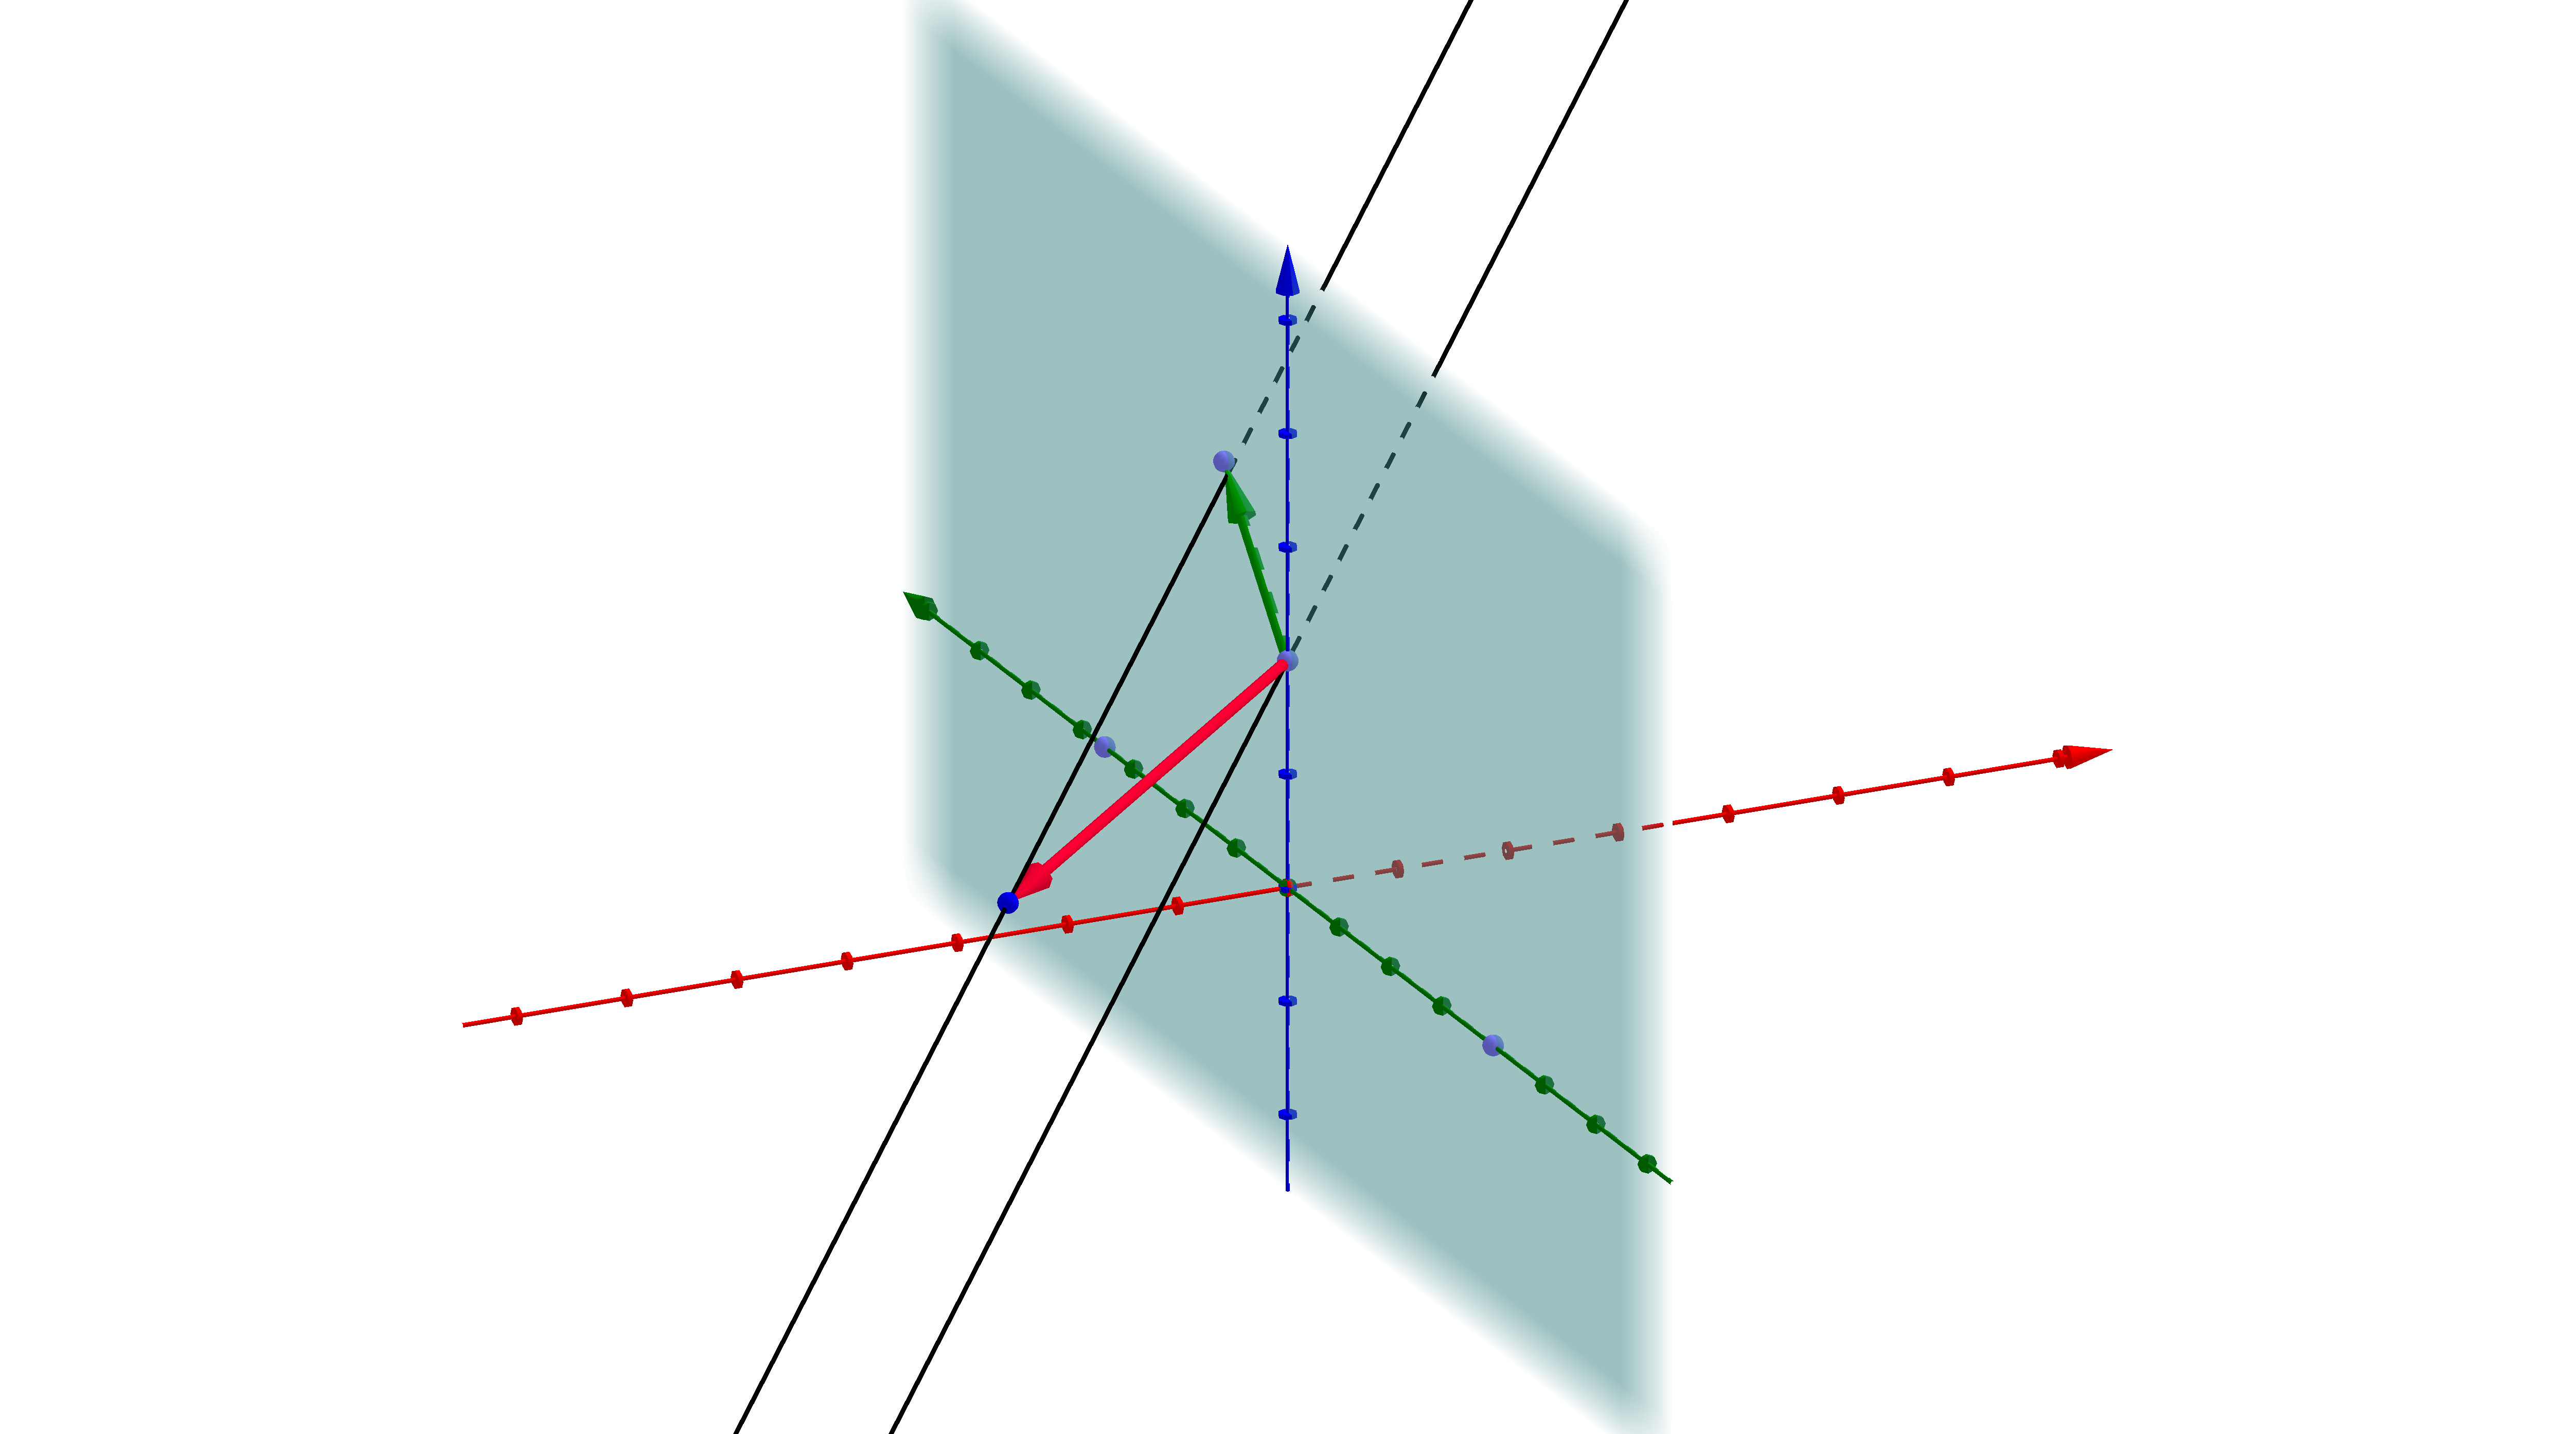
\includegraphics[width=1.0\linewidth]{figures/alignBigger.png}
\caption{The track correction matrix will take as input the track displacement given in red. It will then determine the green vector which is the change on the plane due to that displacement}
\label{fig:TC1}
\end{figure}

\begin{figure}[H]
\centering
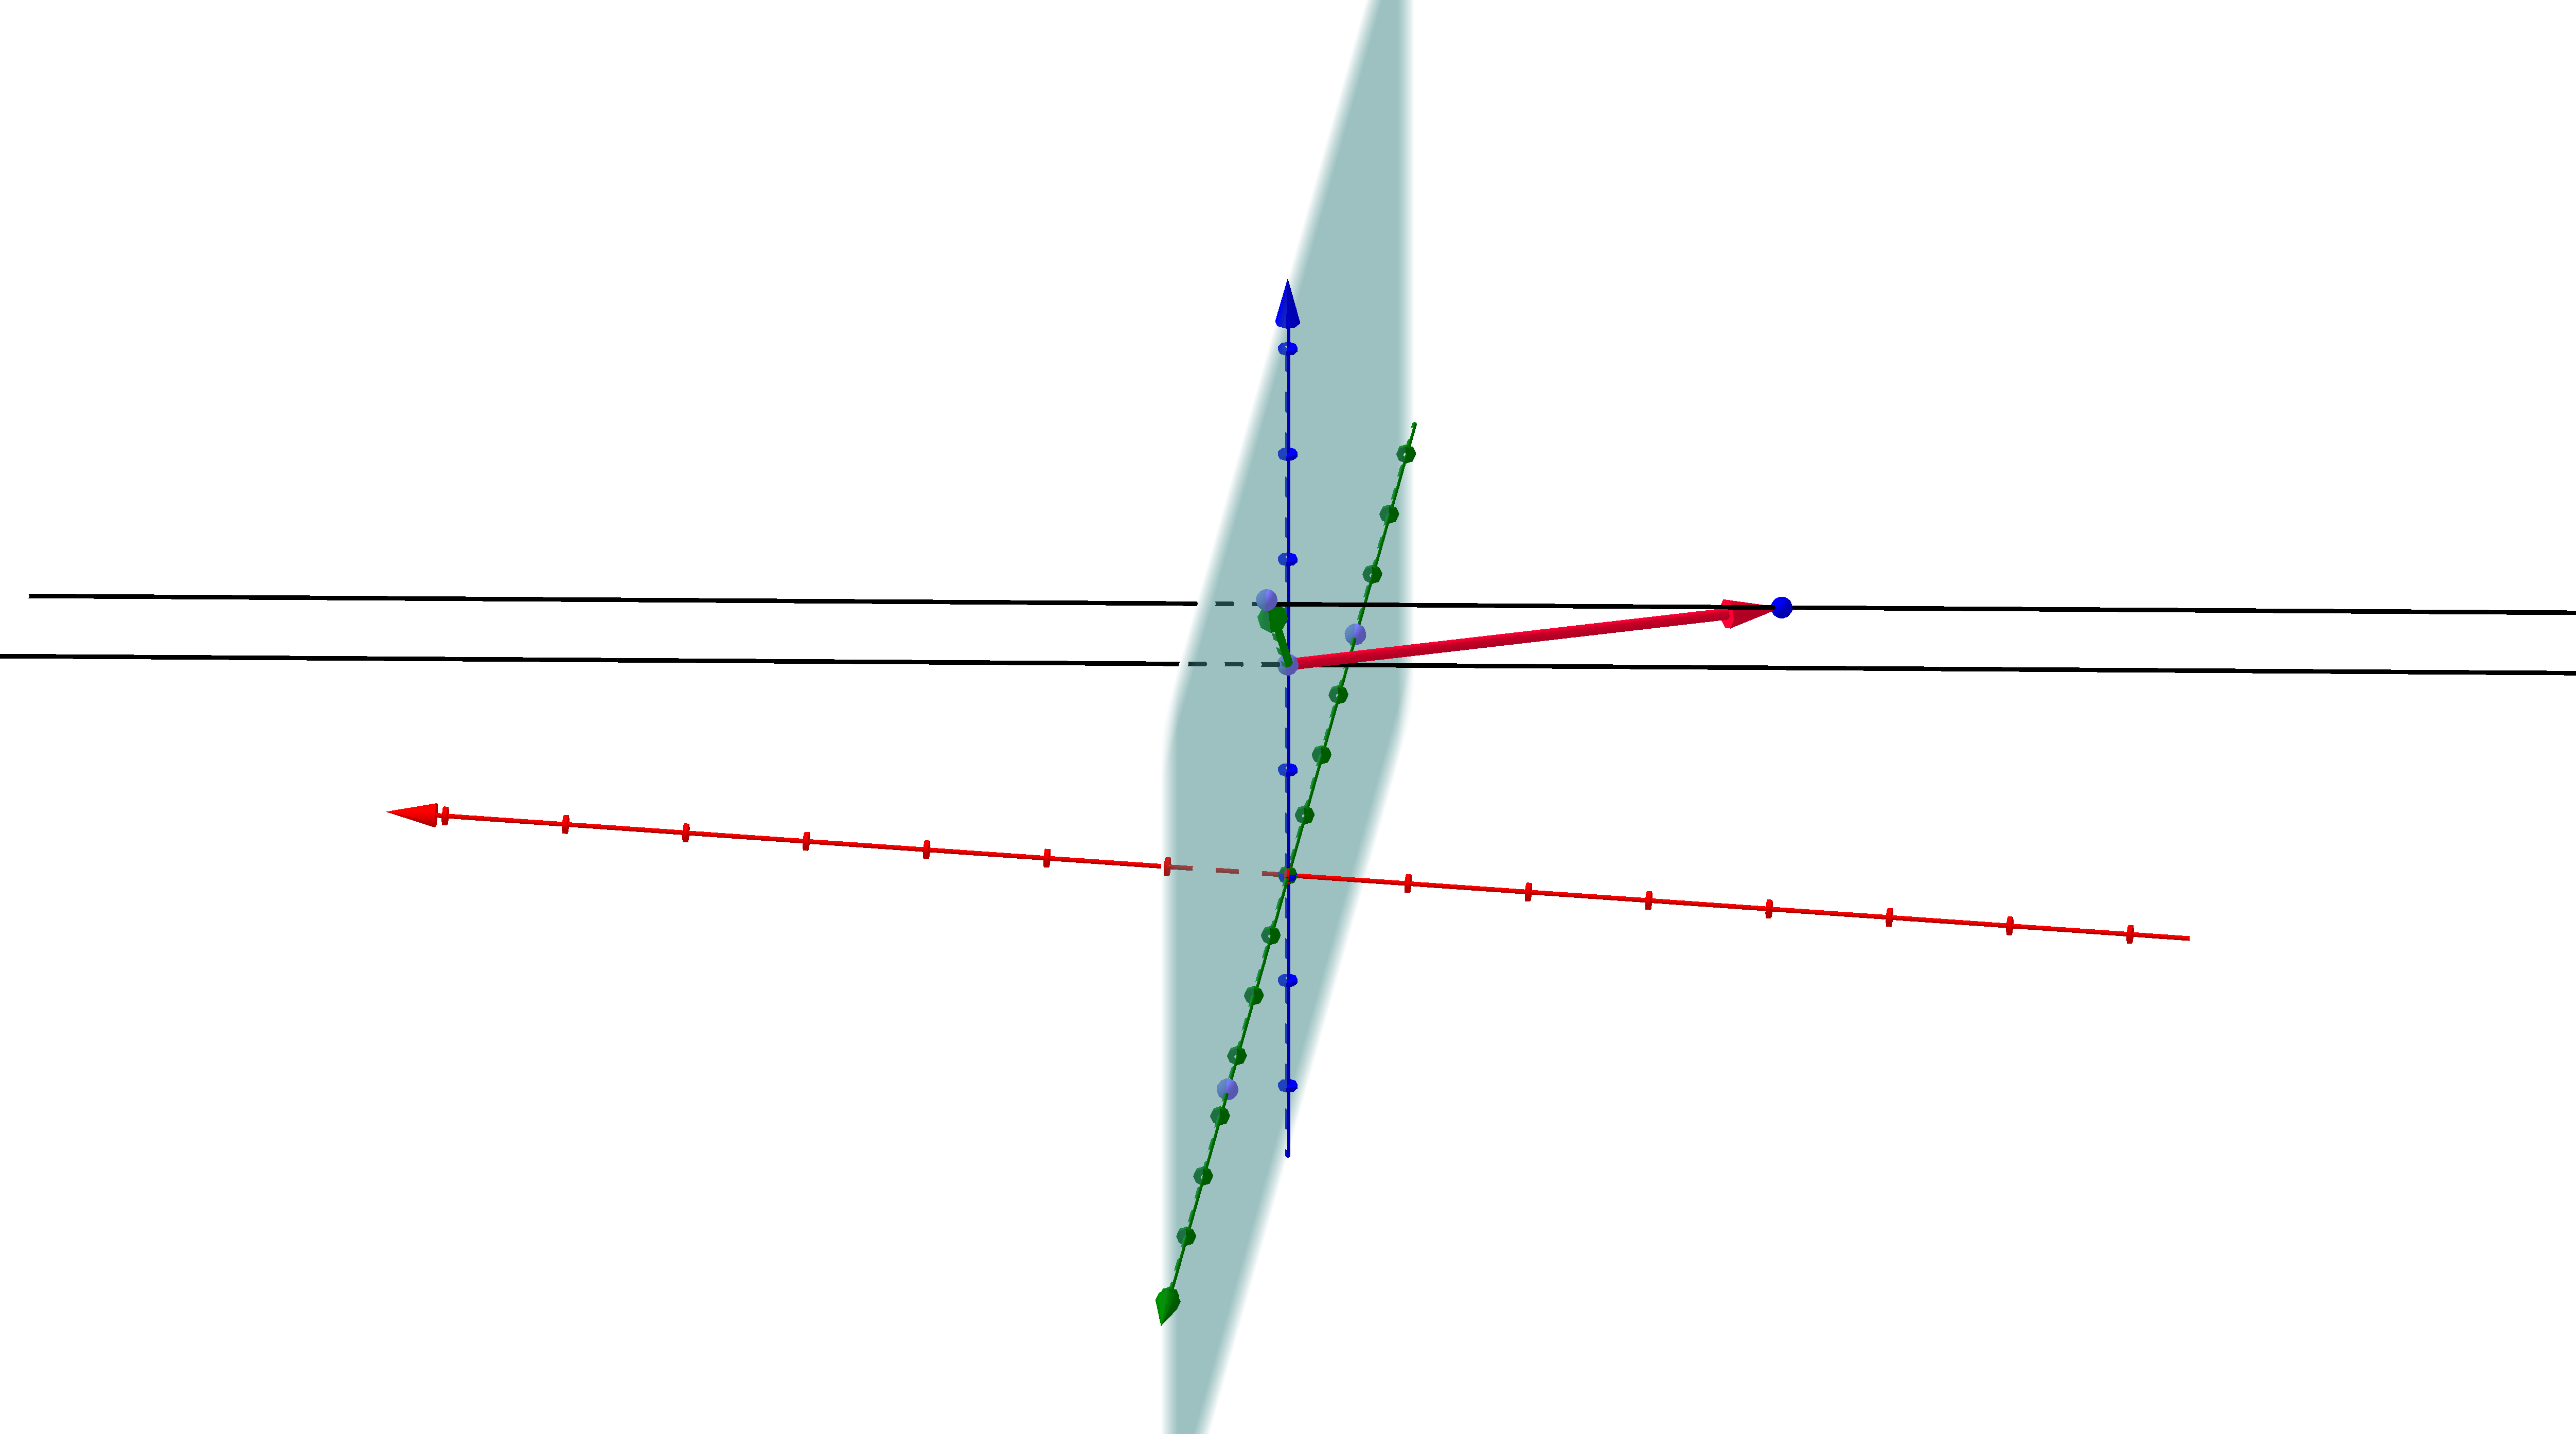
\includegraphics[width=1.0\linewidth]{figures/alignmentBigger.png}
\caption{Same as \ref{fig:TC1} but from a different angle. The green vector is on the plane surface.}
\label{fig:TC2}
\end{figure}

\begin{figure}[H]
\centering
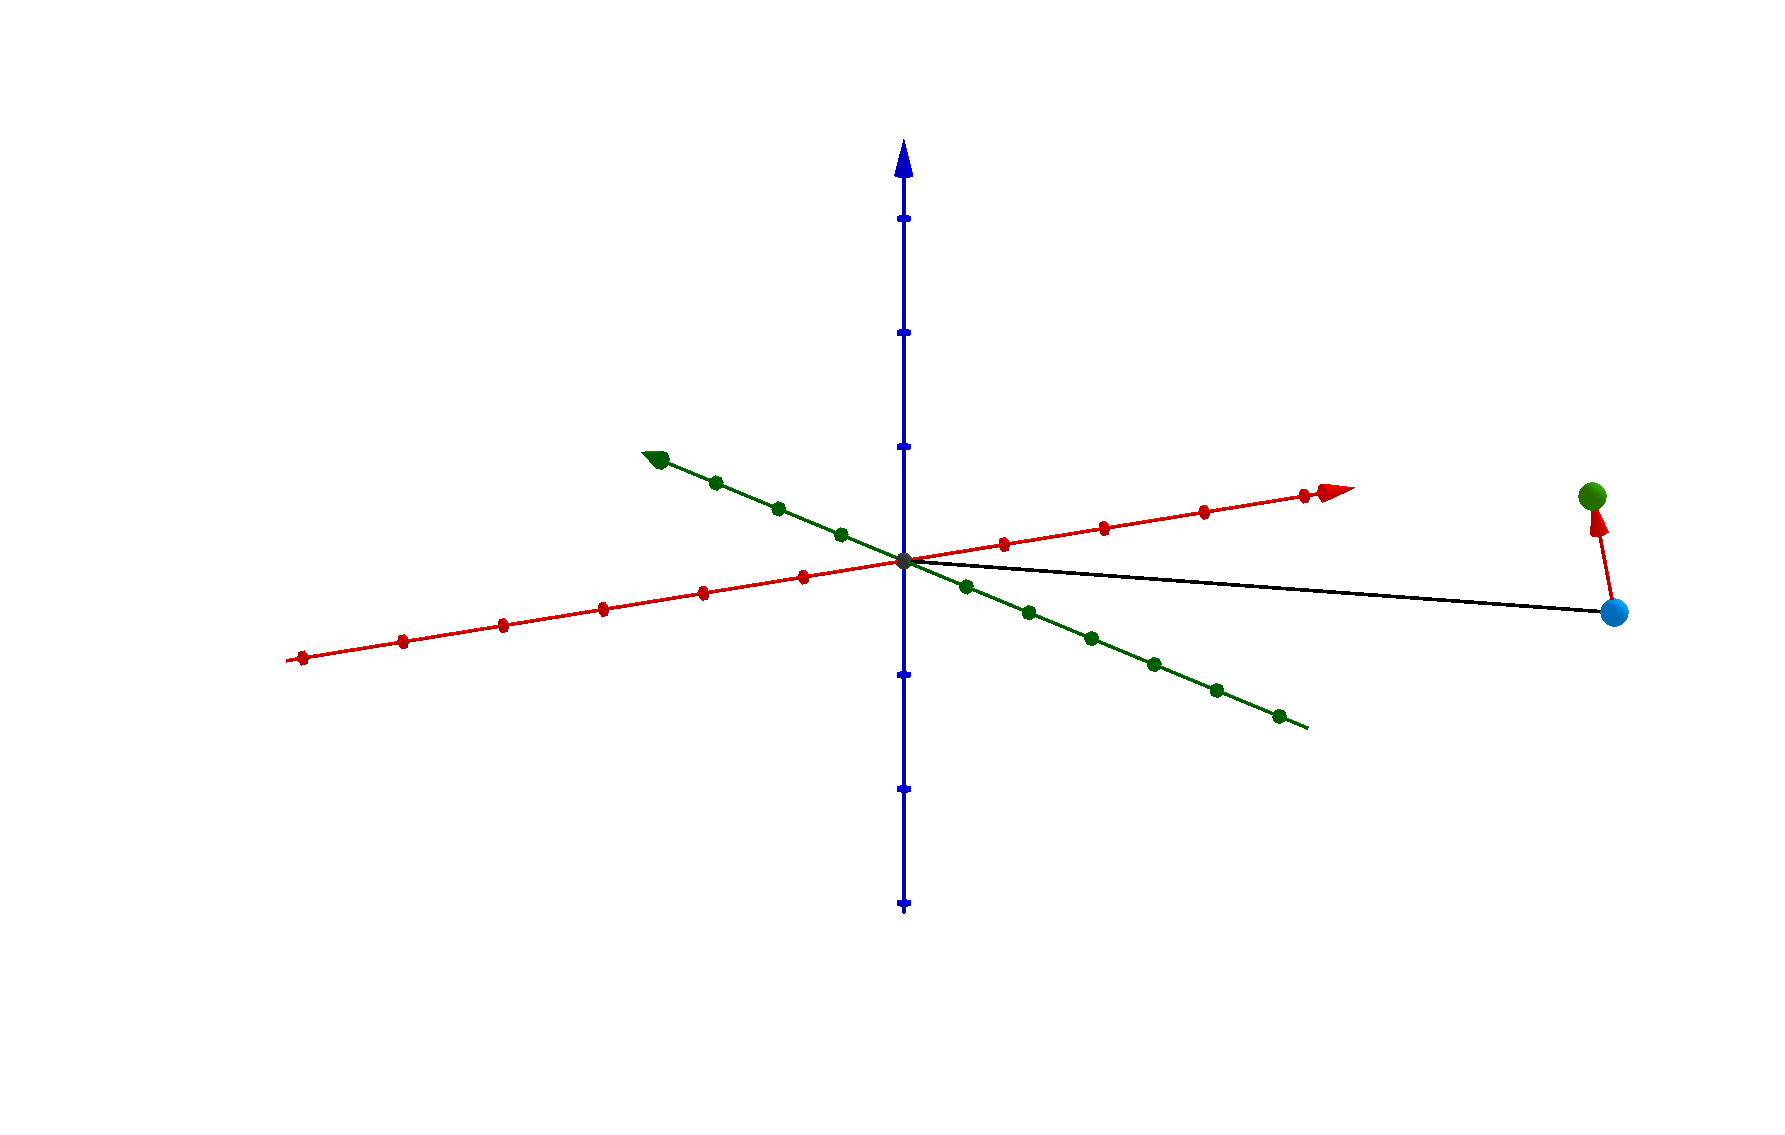
\includegraphics[width=1.0\linewidth]{figures/corrAlign.png}
\caption{The point correction matrix for a particular relative position. The vector is the correction to apply to this point given a certain $(X,Y,Z, \alpha,\beta,\gamma)$ change in the coordinate system.}
\label{fig:CorrMatrix}
\end{figure}

\begin{figure}[H]
\centering
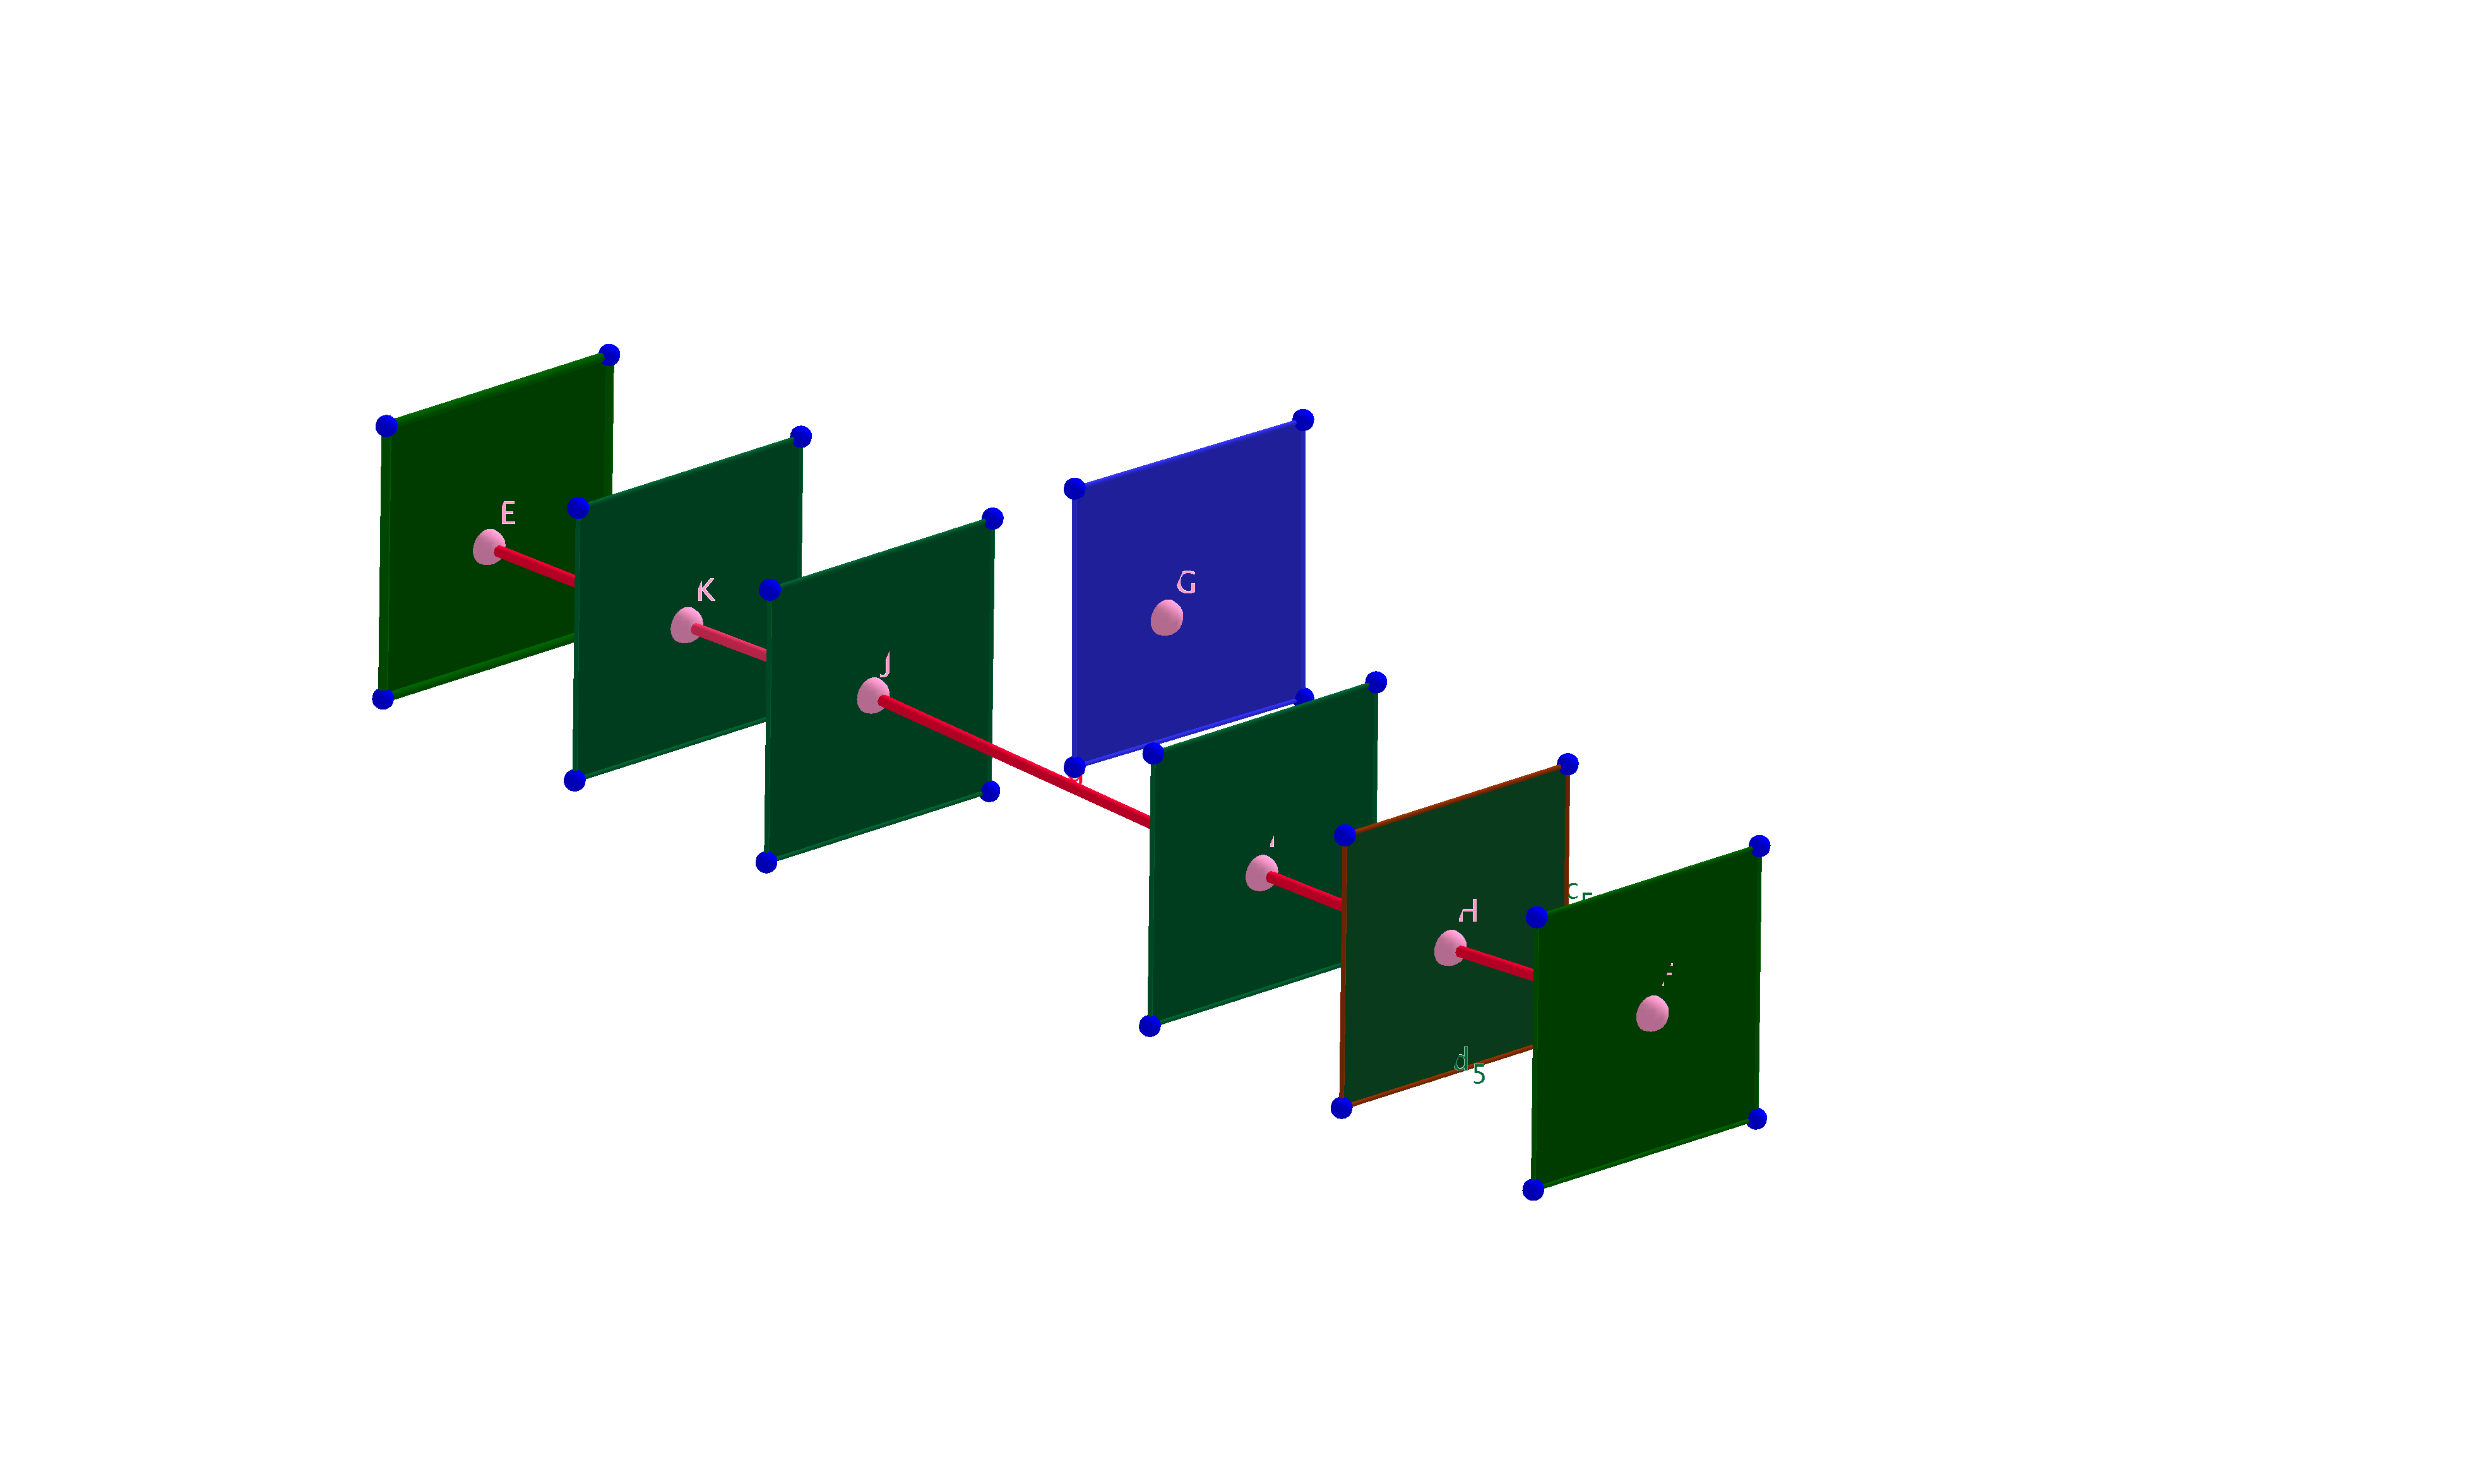
\includegraphics[width=1.0\linewidth]{figures/MisAlignStraight.png}
\caption{Illustration of misalignment with DUT. The transformation of the local DUT frame to the global frame must be wrong so the corrections must be found.}
\label{fig:MisAlign}
\end{figure}

\begin{figure}[H]
\centering
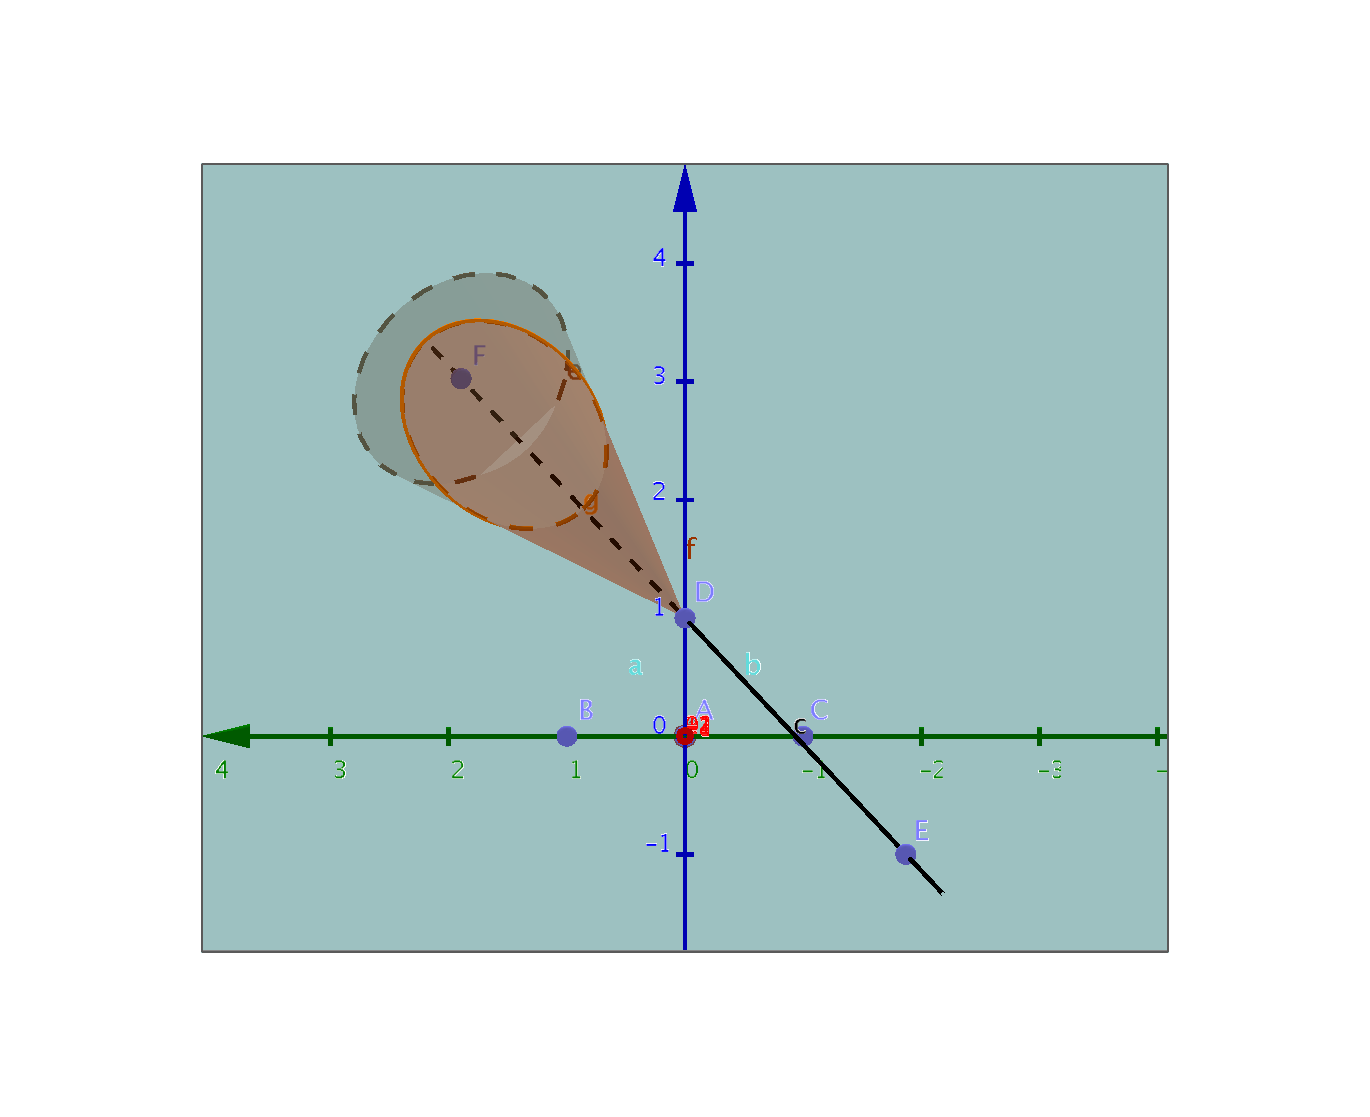
\includegraphics[width=1.0\linewidth]{figures/scatterDownZProjection.png}
\caption{The scattering cone projected on the XY plane of the sensor. The errors on the sensor must take this form to propagate correctly in the z axis}
\label{fig:ScatFrame1}
\end{figure}

\begin{figure}[H]
\centering
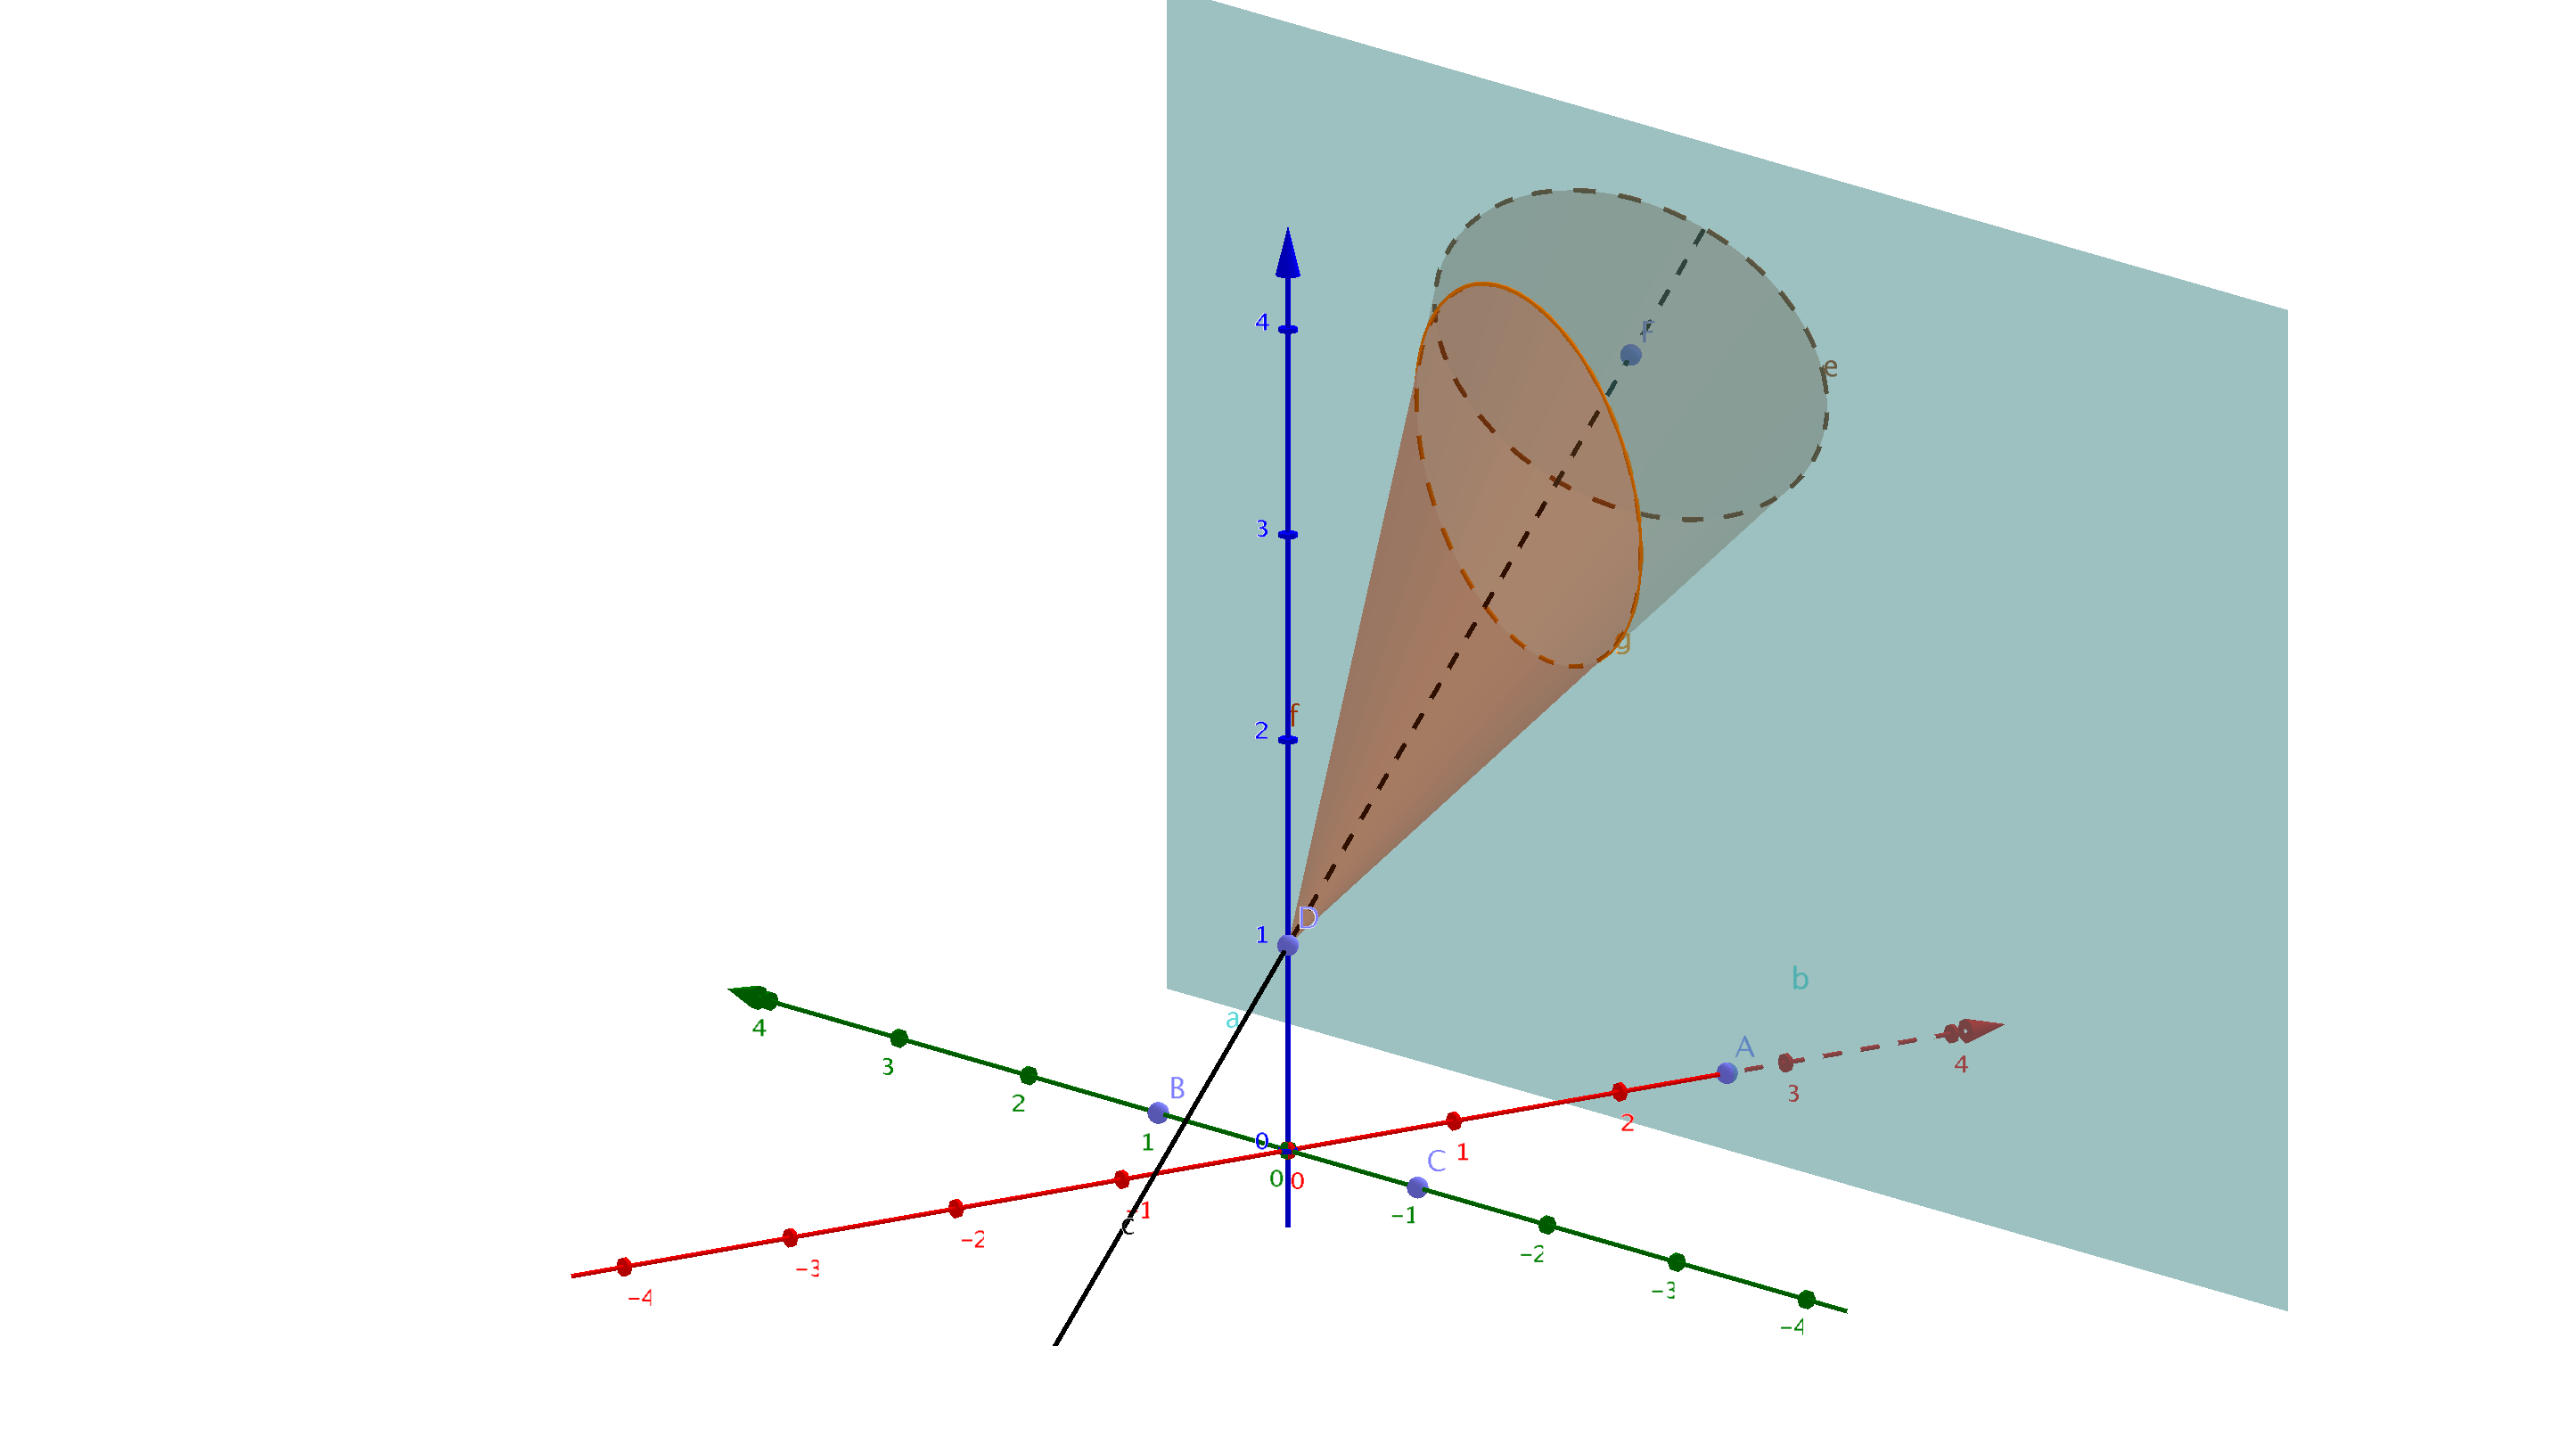
\includegraphics[width=1.0\linewidth]{figures/prop600GoodOffSensor.png}
\caption{The same as figure \ref{fig:ScatFrame1} from a different angle.}
\label{fig:ScatFrame2}
\end{figure}

\begin{figure}[H]
\centering
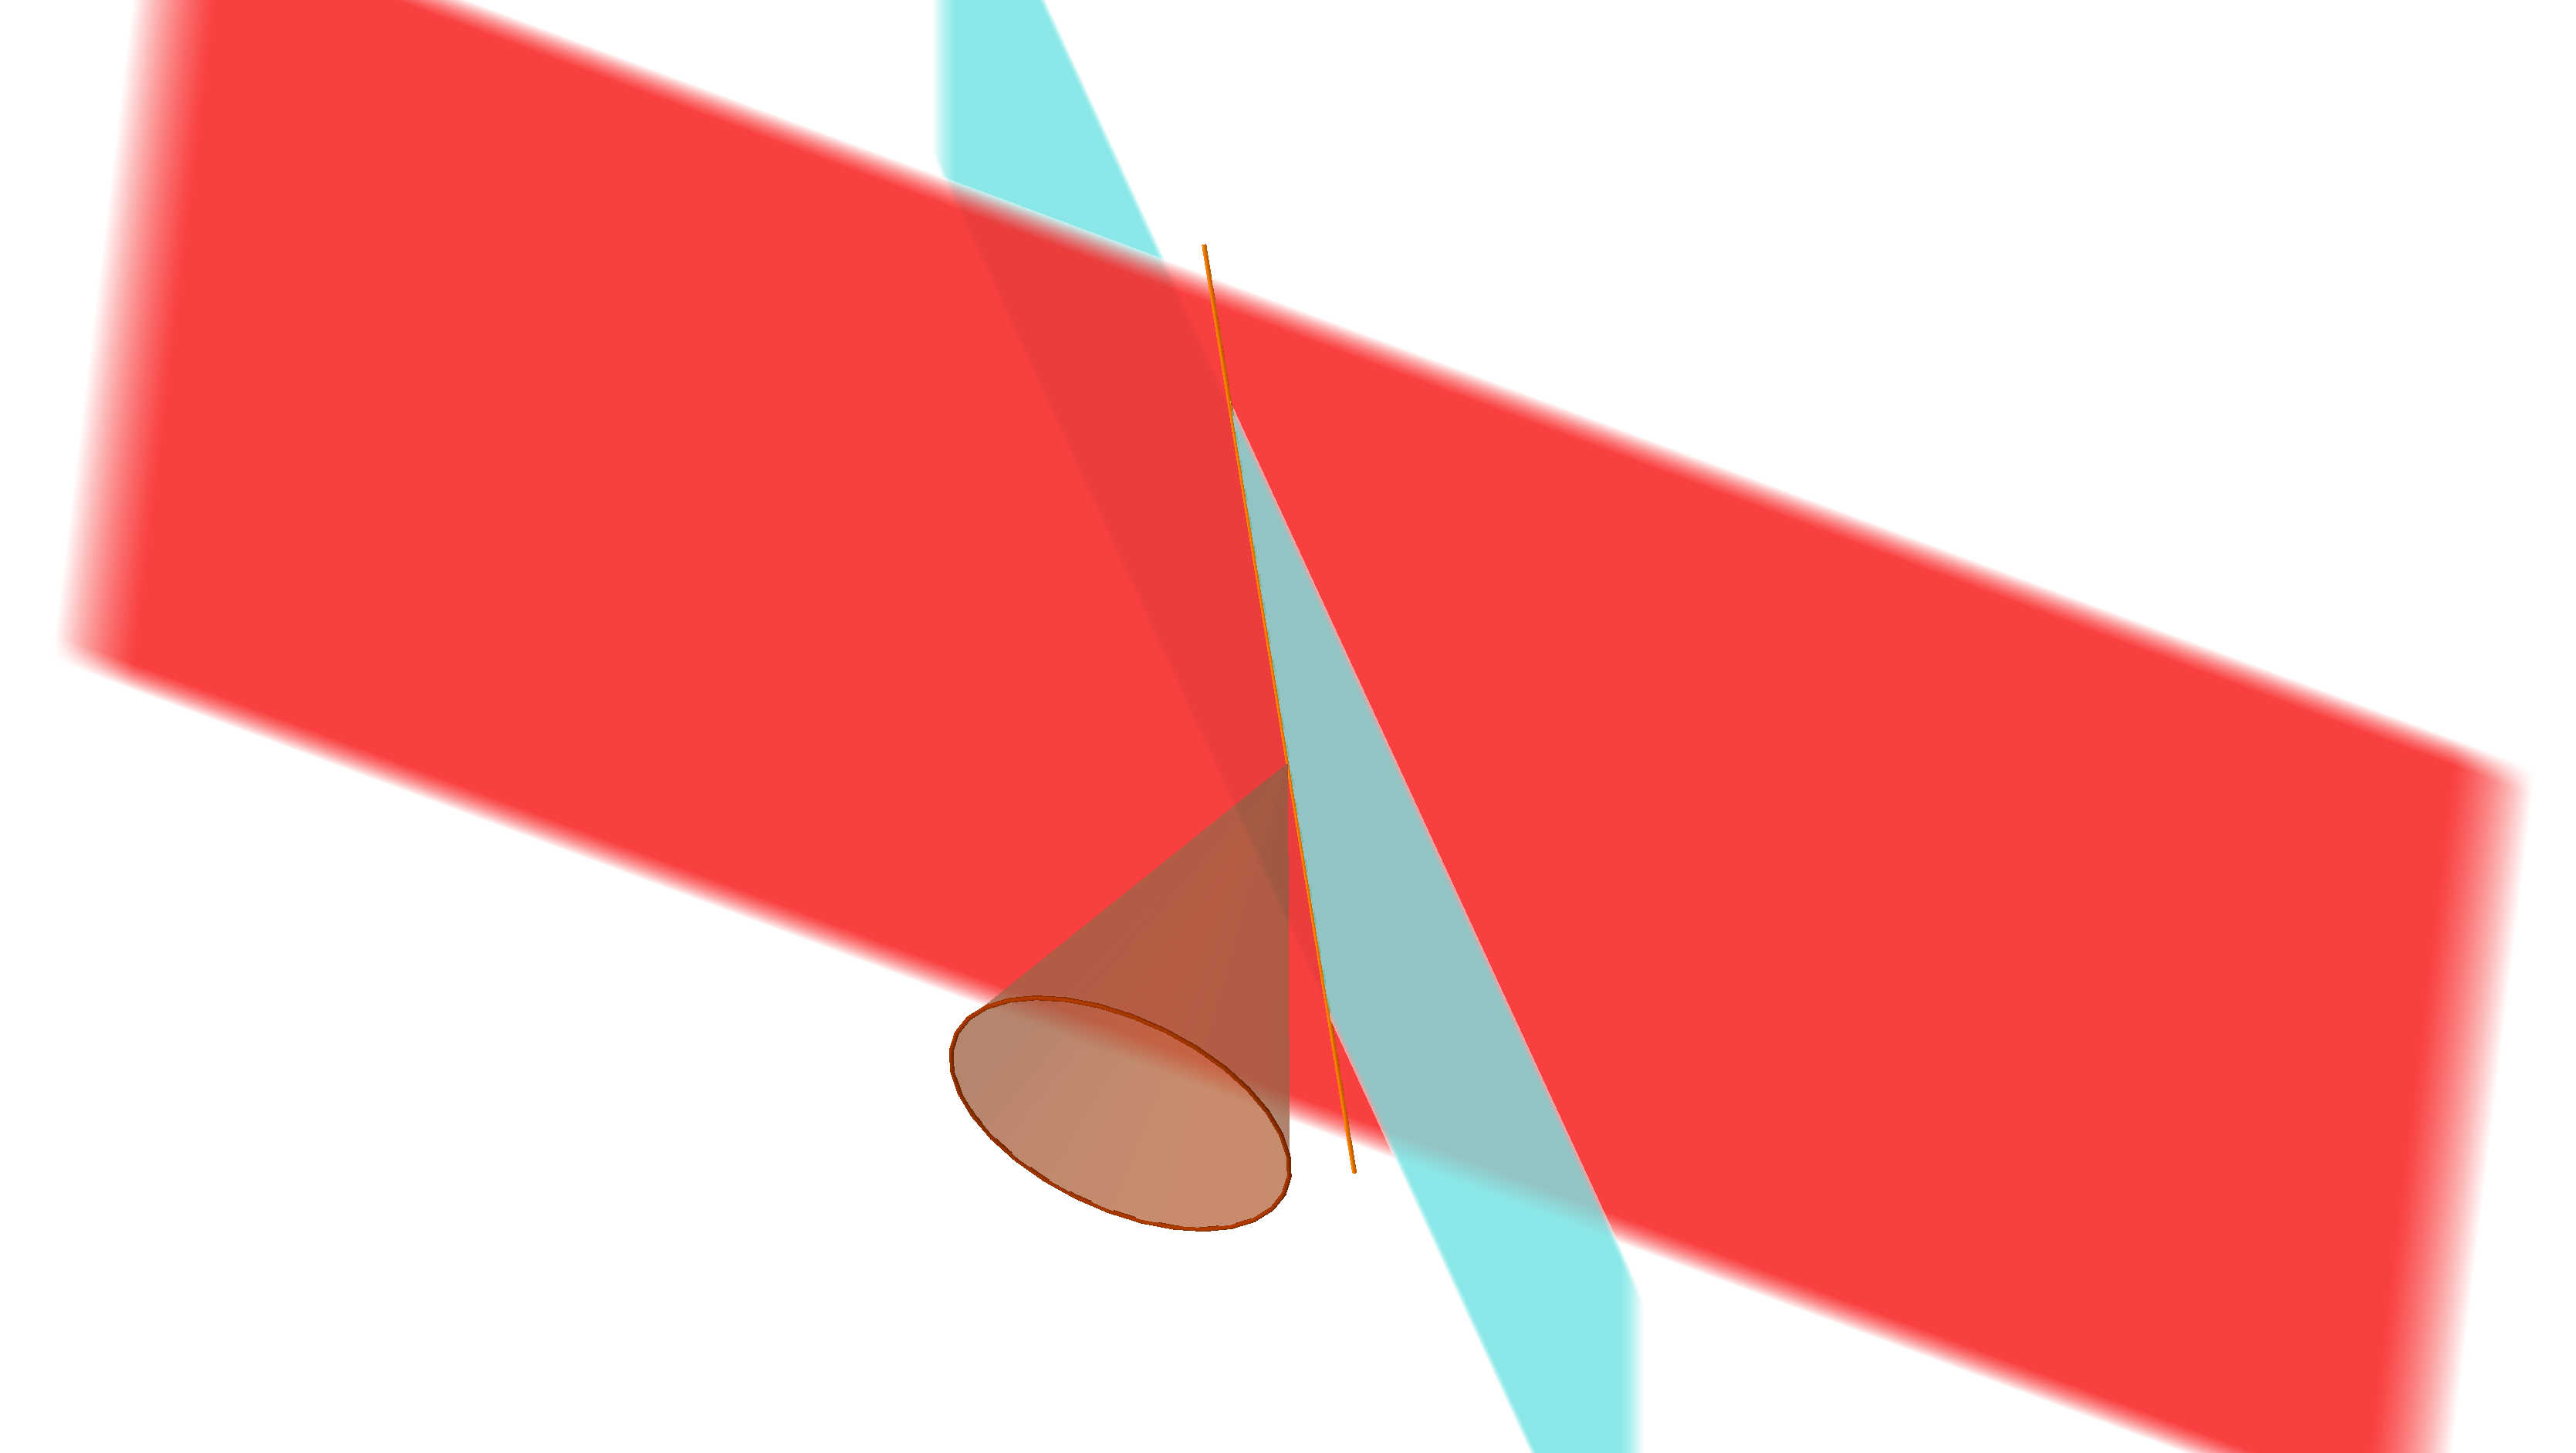
\includegraphics[width=1.0\linewidth]{figures/propGood600.png}
\caption{The scattering frame is the red plane which is perpendicular to the track. The blue plane is the sensor surface. Compare the circular cone which has a diagonal error matrix to the ellipsoid which is non diagonal. This ellipsoid is better seen if the XY plane is propagated downstream with the errors \ref{fig:ScatFrame1}.}
\label{fig:ScatFrame}
\end{figure}

\begin{figure}[H]
\centering
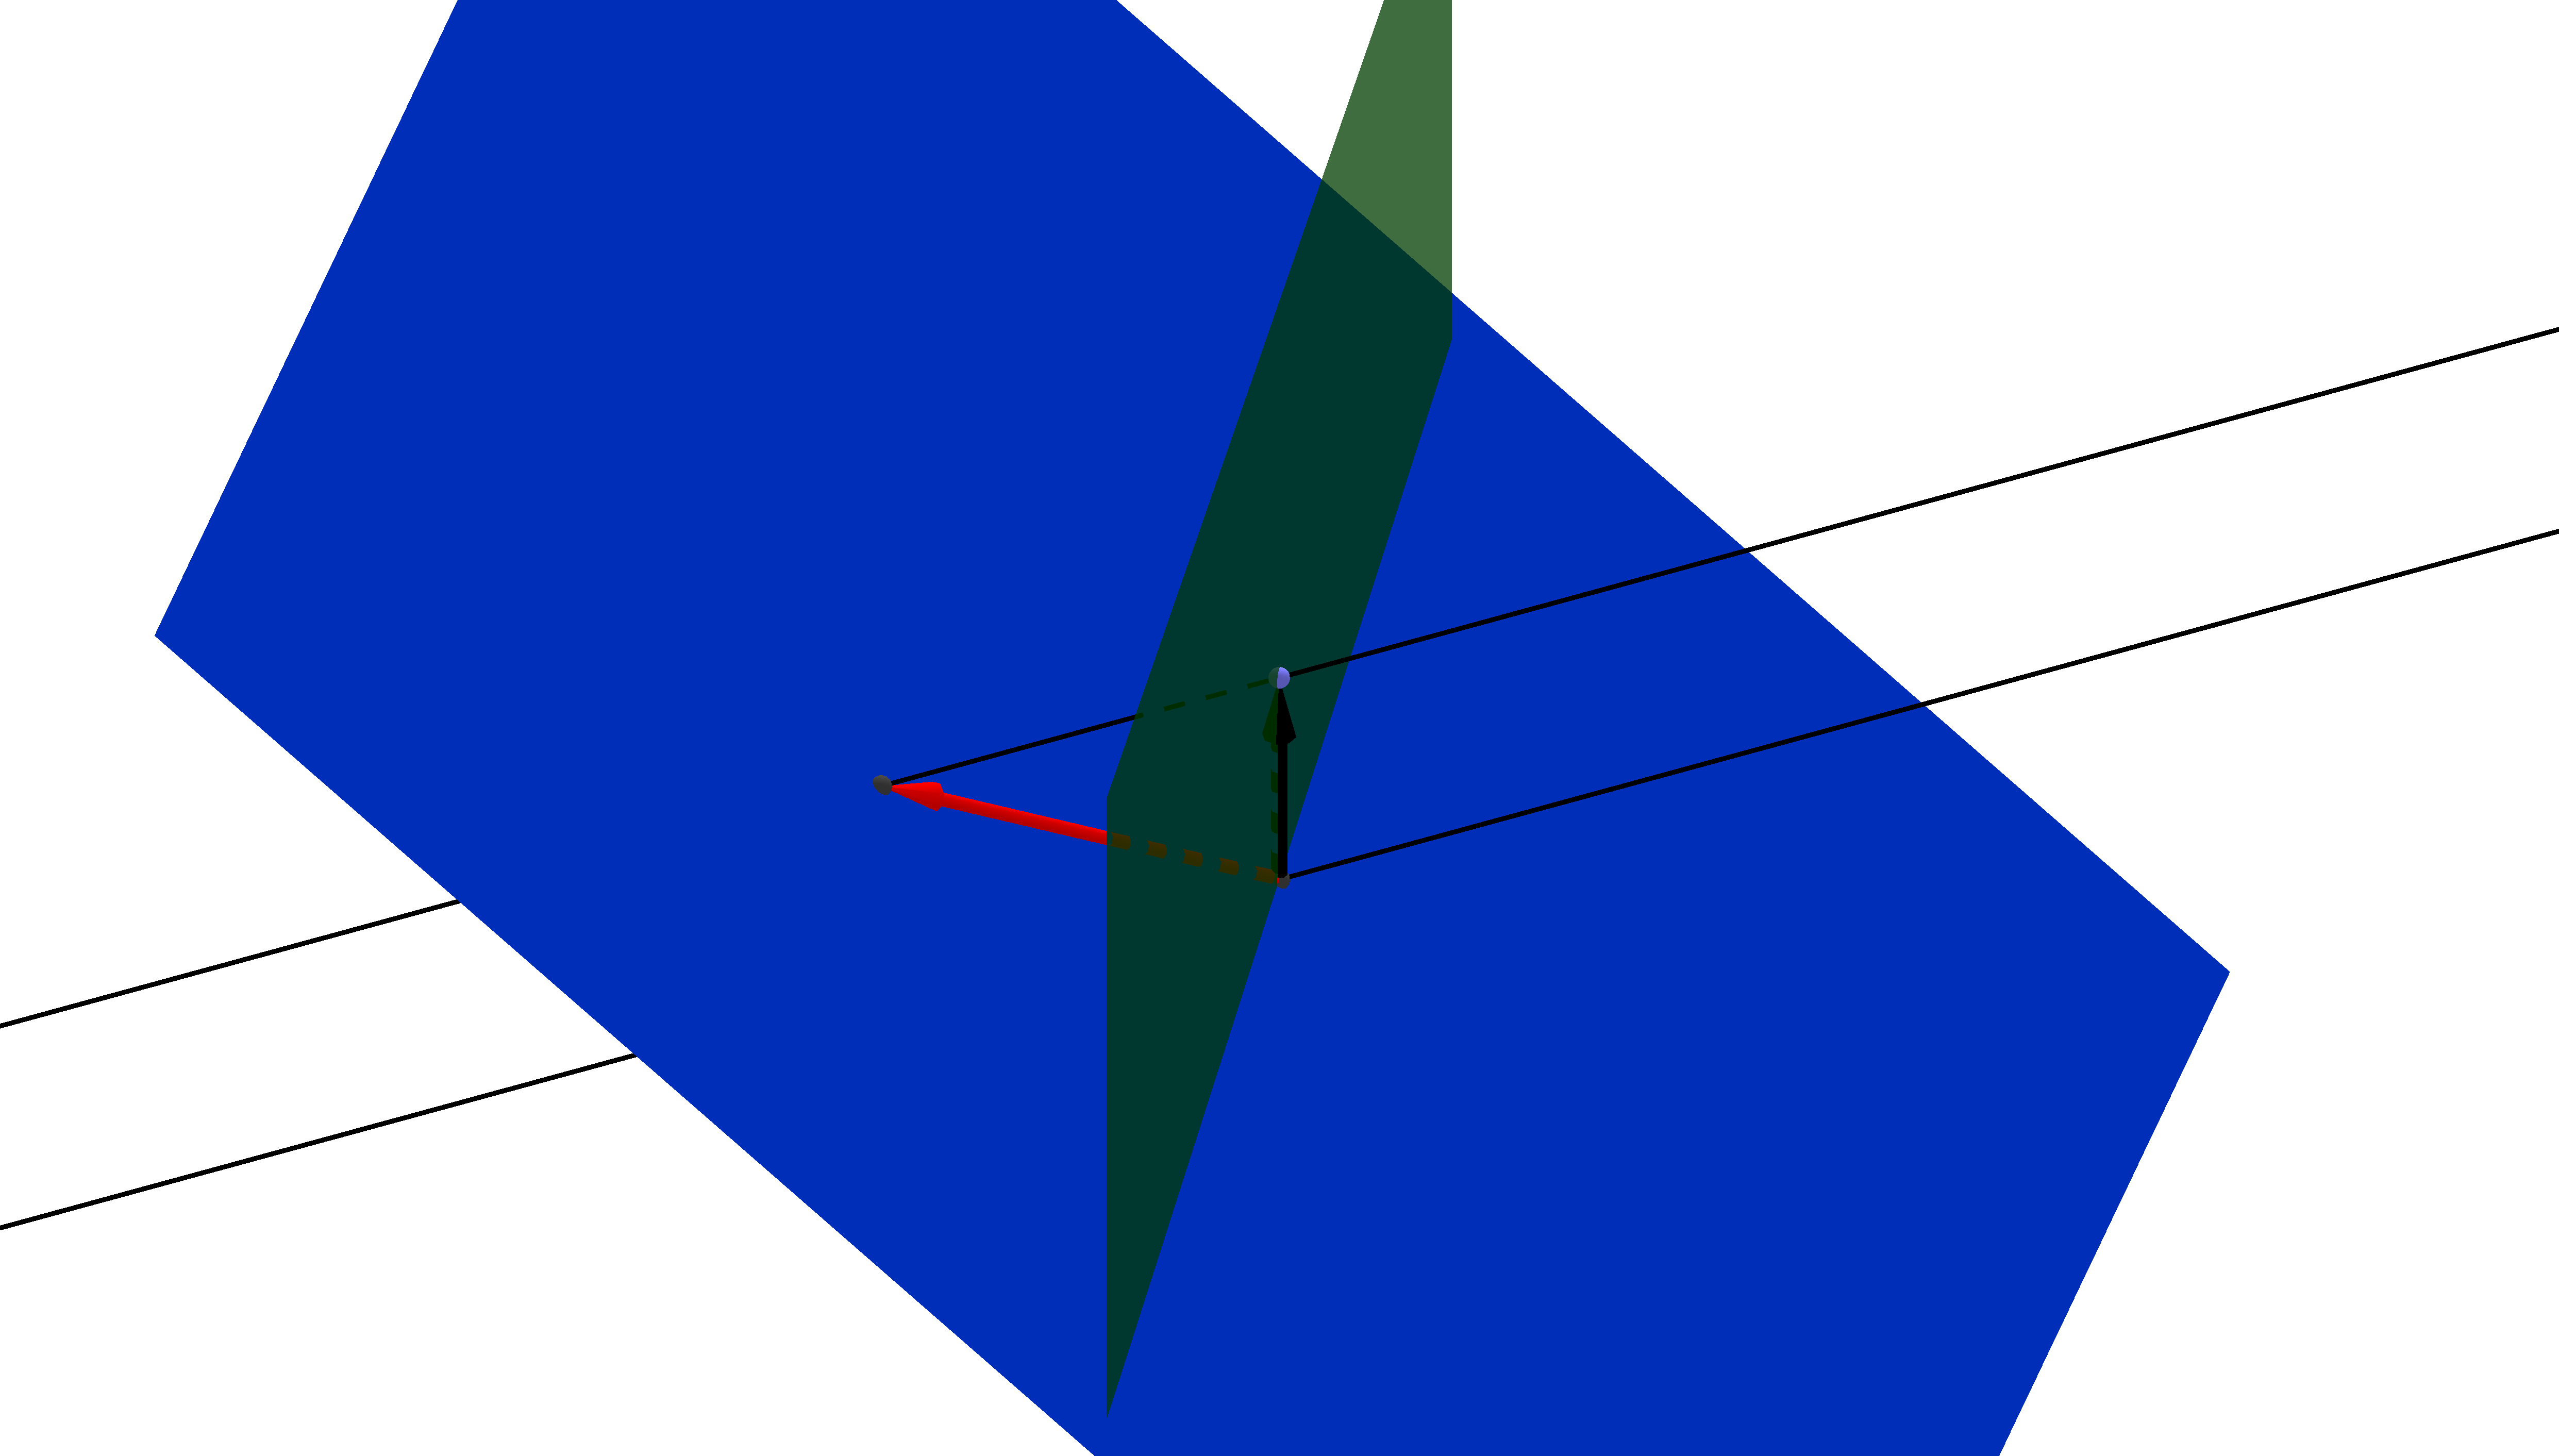
\includegraphics[width=1.0\linewidth]{figures/prop.png}
\caption{The projection matrix will relate the change in residual (black vector) in global XY plane to local XY plane (Blue plane). The propagation must take into account the change in track position intersection. The black lines are the track propagated to the new position.}
\label{fig:Prop}
\end{figure}

\begin{figure}[H]
\centering
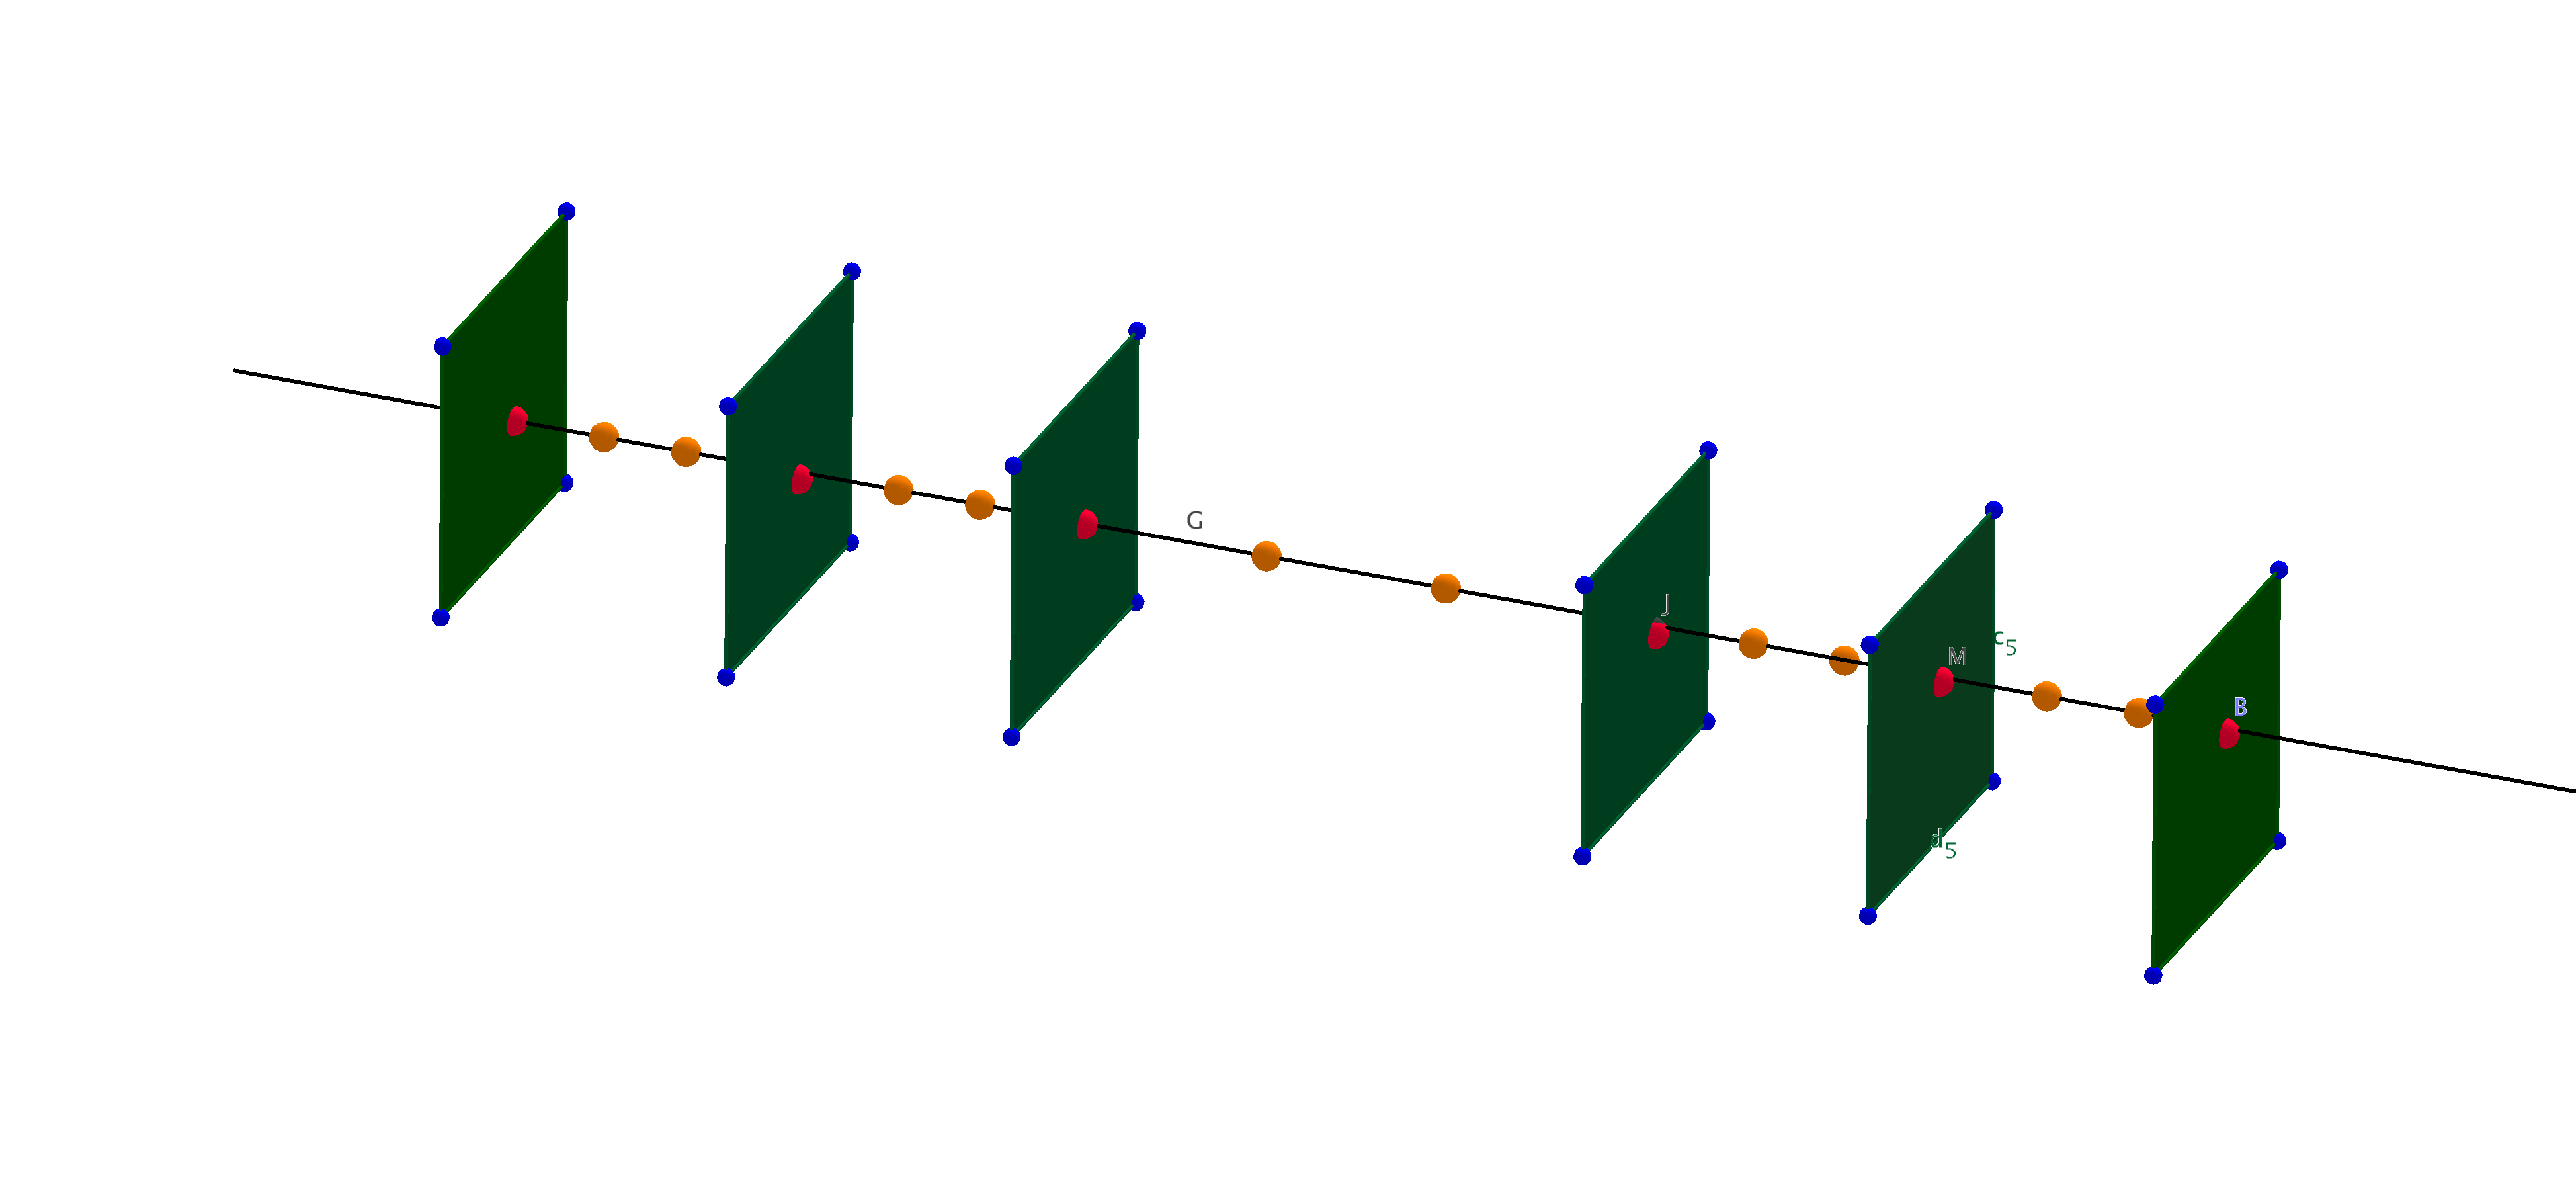
\includegraphics[width=1.0\linewidth]{figures/meas-scat-jac-link.png}
\caption{The red points have measurement and scattering information. The yellow points only scattering information. Measurements are the hit positions in the local frame. Scattering information is the kink angles measured in the local frame. Both have associated errors which must be determined. The Jacobian links all these point together so a change in one will affect a change in another.}
\label{fig:LinkJac}
\end{figure}

\begin{figure}[H]
%\centering
\hspace{-2.5cm}
\subfloat{\label{fig:beamE5B1} \includegraphics[width=0.65\linewidth]{figures/beamE5B1.pdf}}
\subfloat{\label{fig:chi2E5B1} \includegraphics[width=0.65\linewidth]{figures/chi2E5B1.pdf}}
\caption{Figure \ref{fig:beamE5B1} shows the beam energy for a range of pattern recognition inputs, with estimated beam energy 5 GeV and magnetic field 1 T. A cut of  $chi2/ndf > 5$ is made to remove poor tracks for figure \ref{fig:beamE5B1}. Figure \ref{fig:chi2E5B1} shows the chi2 distribution for each fit. }
\label{fig:energy0}
\end{figure}

   

With the set of hits which make up a track determined, the most likely track which produced this collection can be deduced. This track will be in a general case curved (due to magnetic field) and have kinks at points (due to scattering between planes and all other material on the trajectory). The most likely track will be dictated by the spatial resolution of the hit on each detector and the scattering material between each measurement sensor. How this information is combined to form a single track varies, with each method having it's own accuracy. However, a few general principles can be conveyed which are common in all. 
\begin{changemargin}{1em}{2em}
Approximate all the scattering by a series of scattering points. Each point will cause the trajectory of the particle to change due to modelled scattering and can be placed at any location. The kink angle - the angle change of the particles trajectory at that point - will depend on the modelled radiation length at that point. More radiation length will make large kink angles at that point more likely in the final track model. The modelling of the radiation length will vary from the actual radiation length at that physical point due to the granularity of the scattering points, which is a subset of all points on the trajectory. Each scattering point is used to model the radiation length of all points on the trajectory. This approximation is accurate for most mediums with just a few points, but the more inhomgeneous, the more points required for a more accurate track prediction. Radiation length is defined with relation to the density of the material and energy of the particle. The full radiation length of the particle trajectory must be calculated then split between the scattering points of the trajectory. Each point will get a different amount depending on its physical distance from all near by mass. This way of calculating radiation length is important since it deals with the non linearities within the corrected Highland formula.      

With the ability to create a kinked trajectory the hit information is introduced with an estimated spatial resolution which will vary from hit to hit. This can be thought of as a measurement point attached to the measurement plane (the plane defined by the hit pixels or strips) which is part of the trajectory of the track. The measurement points will likely not form a straight line. With the scattering points a track can be formed which best lines up with the measurement points. However, considerations must be made on how large each kink can be made to bend towards each hit. Consider a system with a very large radiation length, then the most likely track is through each hit even if the hit resolution is very poor. As the radiation length decreases to zero, the kinks decrease in angle for all points and the most likely track tends to an unbroken curved trajectory. When the radiation length estimates kinks to bring the track close to the hit within the hits resolution, i.e close but not quite on the hit, the real fun begins. Now the most likely track falls in a no mans land, between the perfect curve and the perfect intersection of all hits. This track can only be determined by use of the precision of the kink angles and hit positions. This precision is determined as the inverse of the covariance matrix and must be propagated from each point to all others. This propagation will link each point with its precision to all other points under some coordinate system. This system is arbitrary, however different systems will have different precision matrices and varying degrees of complexity for propagation.  

Lastly, with all the points linked together with the correct propagated precision and hit information the most likely track can be found. It's advocated that the idea of a track model is kept in mind. So the calculated track is the most likely to have give that series of hits given the prior information of the hit position and radiation length: The track fit is as good as the information provided.   
\end{changemargin}

The creation of the most likely track is all well and good when you know where the hits are positioned. However in most cases life is not that simple. At a testbeam it is very difficult to place a detector in a location known to a few micron. Therefore when hits are identified on a plane, only the approximate location of the hit - to $\approx 1$ mm - can be identified. The planes must be moved to their correct locations with micron precision to perform track fitting. To gain this level of precision a chicken and egg game appears: The unaligned planes with hits that produce tracks can be used to determine the misalignment, however the planes must be roughly aligned to find the legitimate hits that form a single track. This is solved by splitting the alignment into two parts: pre-alignment and the final micron level alignment. Pre-alignment corrects shifts to $\approx$ 0.5 mm using the correlations between hits on each plane. This brings the planes close enough to expect the pattern recognition to find the correct tracks (This of course depends on the pattern recognition and environmental factors such as the occupancy per event). The final alignment uses all the track information discussed and then adds the information on how the movement of the measurement planes will change the position of the hits. Now the most likely track can be found by moving the kinks and moving the planes (Contrast this with track fitting which only the scatterer points could move). The correct position of the planes is the one in which all tracks on average maximise their likelihood.      




\subsection{General Broken Lines (GBL) and EUTelescope}
When considering the problem of track fitting the creation of measurement and scattering points is common to all techniques. However, how these points are related varies, an example would be the use of a  Kalman filter. A Kalman filter is used for many different purposes outside track fitting. However this technique can be combined with a suitable jacobian to link points together under a certain coordinate system to produce an effective track fitter. The salient point to note is that the linking of points with a basic Kalman filter is usually between the position and the incidence of the hits on the measurement planes (The curvature is also used which is a single parameter for the full track). As each parameter is changed this changes the parameters of all the other points on the trajectory. This method works and is effective, however is not using the underlying track fitting problem's symmetries. Consider how track fitting was described in section \ref{patTraAli}, with a series of scattering points moving in space to produce a broken curve which best fitted a series of hits. The scatterers' positions are what must be determined, the incidence angles and curvature are afterthoughts even if they are of the most use for the final analysis. 


The General Broken Line (GBL) algorithm does just that: It takes all the information needed expressed in some coordinate system and breaks this down to the relationship between scattering points only. When this is done a simplification of the fit is apparent, with many elements of the final matrix which must be inverted being 0, this is the symmetry present in all track fitting. The most likely position of the scattering points are then determined and this is then related back to parameters such as the incidence and curvature \cite{GBL}. This process is mathematically equivalent to a Kalman filter but is clearly computationally different. 


\section{My contribution}

A C++ implementation of GBL exists and has been integrated within EUTelescope. The integration of GBL within EUTelescope goes beyond just a new track fitting model. It aims to allow the same procedure to fit tracks from a plethora of different DUTs, geometric setups and environmental changes. This includes complex pixel arrangements, magnetic fields and arbitrary DUT orientations. To this end many aspects of EUTelescope had to be updated to deal with these issues in a common way. This is discussed in full in the GBL section of this AIDA note \cite{AIDAnote}.

A more practical introduction presented here is to test the fitter in different environments. One important test of a fitter is the effect pattern recognition has on a track fit. The initial pattern recognition estimates of the track should not influence the final fitted track. A way of testing this is to do an energy scan search for different combination of hits that correspond to a different energy. This is done by setting the initial "guessed" energy (E) for the pattern recognition to a particular value and then searching for tracks. Each track will only accept a hit if it falls within a particular radius (R) of it's guess. The initial pattern recognition tracks will be different for each estimate, however the final GBL track should converge to the correct physical trajectory of the particle. 

Data was taken at testbeam at DESY with a set beam energy of 5 and 3 GeV in a magnetic field of 1T. The magnetic field allows the determination of the energy of the particle using the curvature of the track. Figure \ref{fig:energy0} and \ref{fig:energy1} show the estimate energy of each track for the 5 and 3 GeV beam. 
\begin{figure}[H]
%\centering
\hspace{-2.5cm}
\subfloat{\label{fig:beamE5B1} \includegraphics[width=0.65\linewidth]{figures/beamE5B1.pdf}}
\subfloat{\label{fig:chi2E5B1} \includegraphics[width=0.65\linewidth]{figures/chi2E5B1.pdf}}
\caption{Figure \ref{fig:beamE5B1} shows the beam energy for a range of pattern recognition inputs, with estimated beam energy 5 GeV and magnetic field 1 T. A cut of  $chi2/ndf > 5$ is made to remove poor tracks for figure \ref{fig:beamE5B1}. Figure \ref{fig:chi2E5B1} shows the chi2 distribution for each fit. }
\label{fig:energy0}
\end{figure}

Note the beam is expected to have some natural spread which is shown. Also observe the drop in energy which is present in both from the expected energy. This is due to the passage of the particle through material which houses the magnet. The pattern recognition has no effect on the mean of the distribution and each is only wider due to larger acceptance of tracks in different regions.  

\begin{figure}[H]
%\centering
\hspace{-2.5cm}
\subfloat{\label{fig:beamE3B1} \includegraphics[width=0.65\linewidth]{figures/beamE3B1.pdf}}
\subfloat{\label{fig:chi2E3B1} \includegraphics[width=0.65\linewidth]{figures/chi2E3B1.pdf}}
\caption{ Figure \ref{fig:beamE3B1} shows the beam energy for a range of pattern recognition inputs, with estimated beam energy 3 GeV and magnetic field 1 T. A cut of  $chi2/ndf > 5$ is made to remove poor tracks from figure \ref{fig:beamE3B1}. Figure \ref{fig:chi2E3B1} shows the chi2 distribution for each fit.}
\label{fig:energy1}
\end{figure}

\subsection{Upgrade sensors}
\textbf{Add residuals for each sensor. Should fix the title etc for report.}
\begin{figure}[H]
\centering
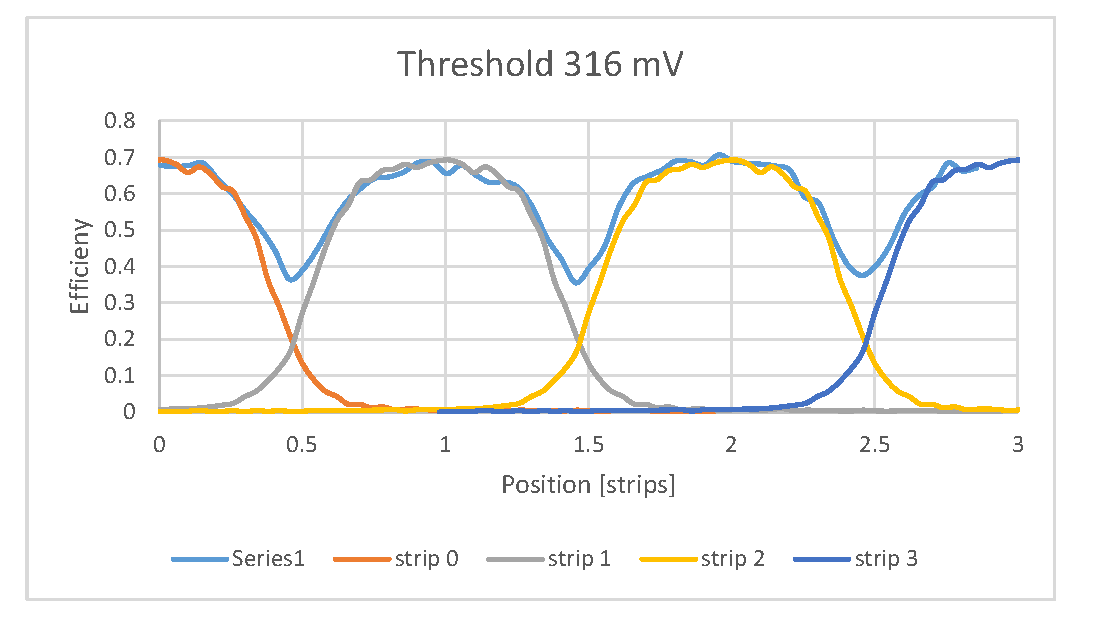
\includegraphics[width=1.0\linewidth]{figures/eff_strip.pdf}
\caption{ATLAS12 efficiency measurements.}
\label{fig:Prop}
\end{figure}

\begin{figure}[H]
\centering
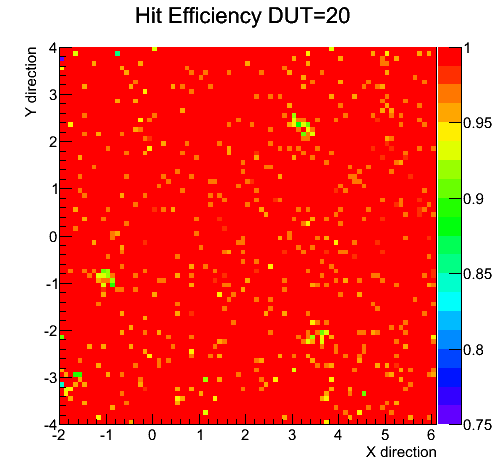
\includegraphics[width=0.7\linewidth]{figures/desy250x50AC_250x50DC_20V20.png}
\caption{250x25 $\mu m$ pixel sensor}
\label{fig:Prop}
\end{figure}

\begin{figure}[H]
\centering
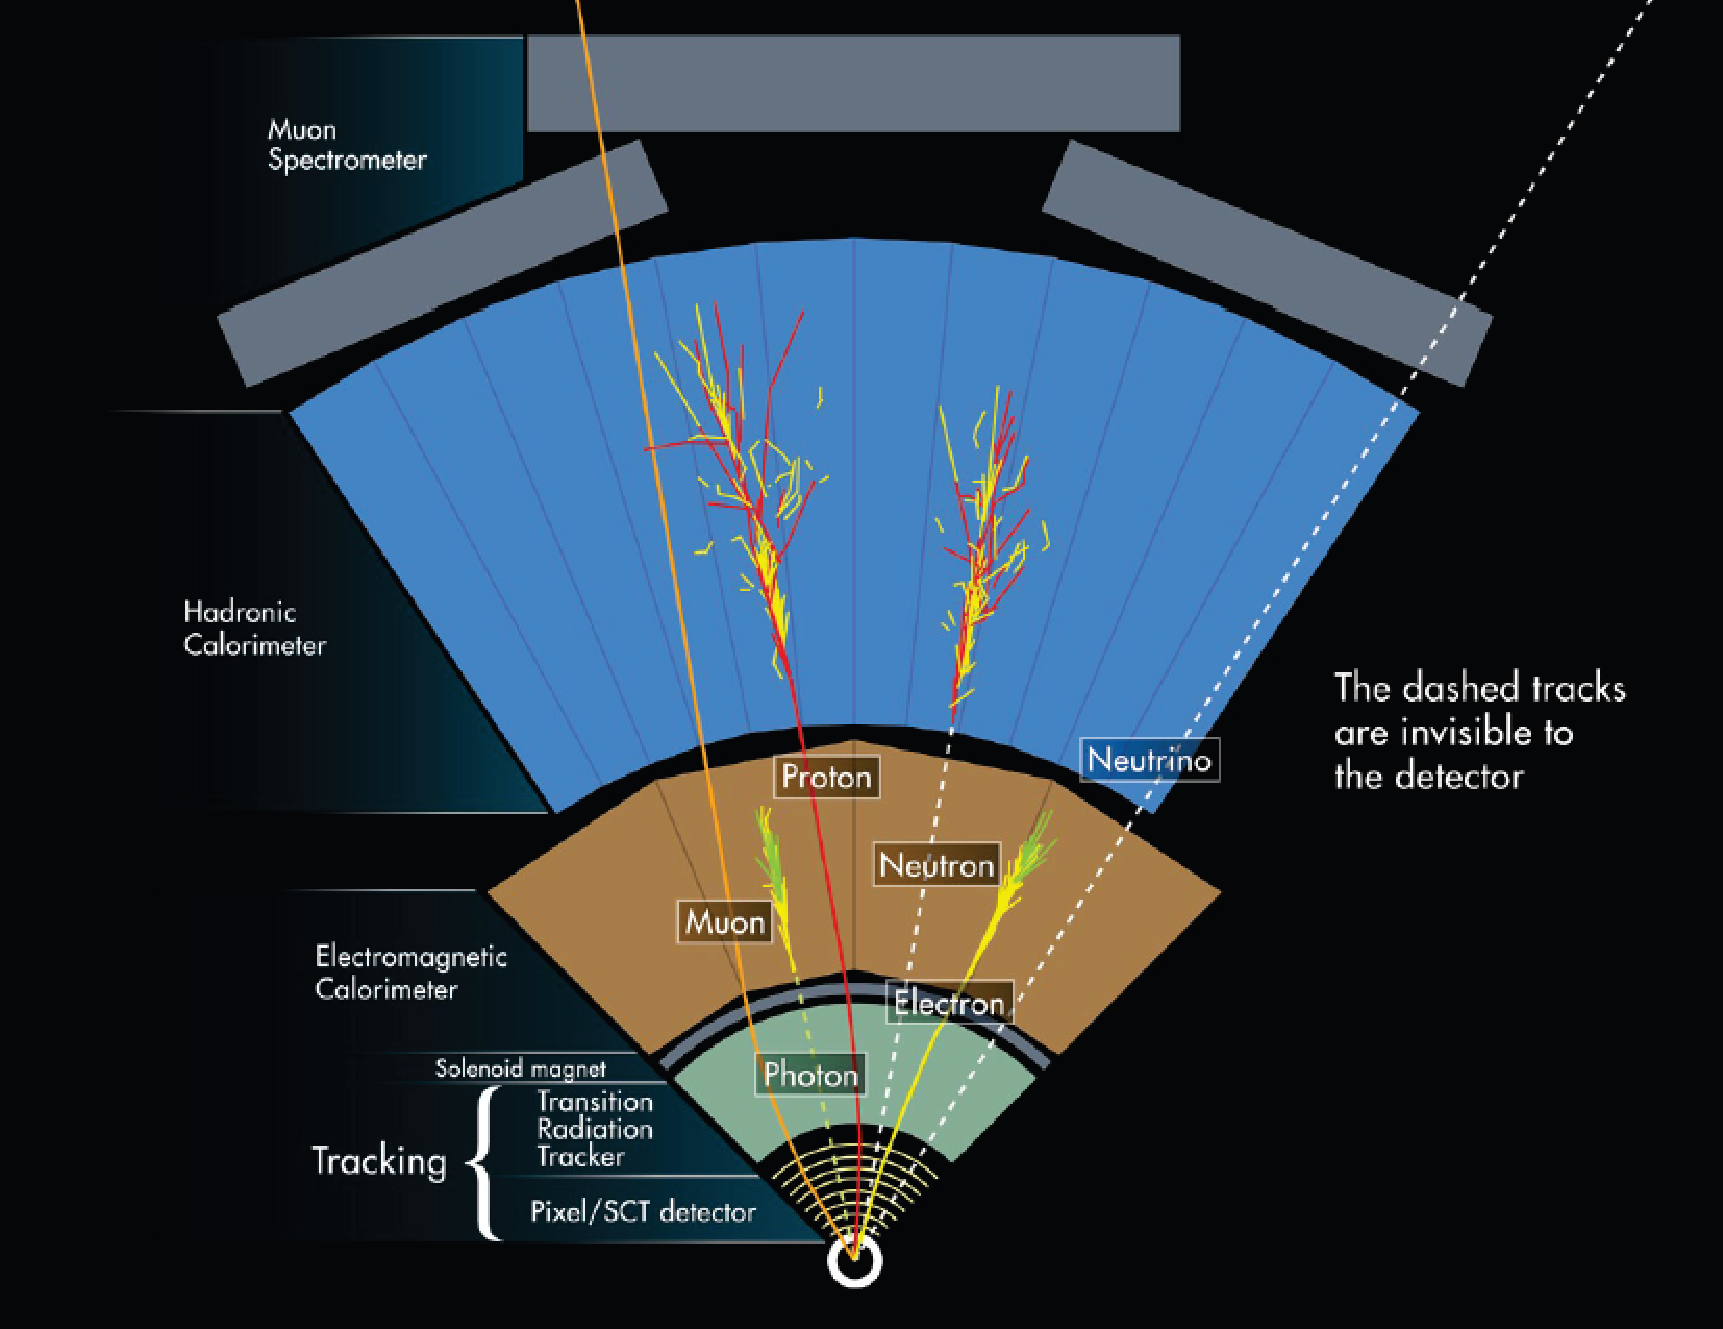
\includegraphics[width=1.1\linewidth]{figures/atlas.pdf}
\caption{ATLAS Experiment �2013. ATLAS images are under CERN copyright.}
\label{fig:Prop}
\end{figure}
\subsection{Track Fitting} 
<This should go with above, pattern recognition, then all the frames, the this, this GBL in particular.> 
Once position and scattering information is propagated throughout the detector system, the next concern is the estimator to use to determine the most likely values of the fit parameters. 
\subsection{ATLAS ITK Upgrade}
The arrival of HL-LHC with a instantaneous luminosity of $5\times10^{34}cm^{-2}s^{-1}$ will bring with it many opportunities but also many challenges. The increased luminosity will allow precision measurements of the SM Higgs couplings. Furthermore a range of new physics signatures can be explored in this new energy regime <Andy blues talk>. The challenges in building the ATLAS ITK:
\begin{description} 
	\item[Radiation Hardness] Sensor and electronics must survive up to $1.6\times10^{15} n_{eq} cm^{-2}$ over lifetime.
	\item[Occupancy] Occupancy below 1\% in all areas.
	\item[Trigger Rates] 
\end{description} 

In addition the material budget of the detector must be considered due to scattering effects which introduces increased uncertainty on the reconstructed track.

\subsection{Prototypes}
Should add information on each of the examples. 

\subsection{Radial Strips}
\subsubsection{TGeo and Coordinate transformations}

%Put in manual 
Any pattern recognition can be used with the GBL fitter. This is essential to make the procedure as generic as possible since different forms of pattern recognition are needed for different situations. The only requirement of the GBL fitting processor is a collection of hits which form a track. Parameterisation of the track is done internally and is not required by any new pattern recognition. A basic clustering pattern recognition can be used with the GBL fitter. However the new triplet finder method has been shown to perform better in nearly all scenarios. Therefore this is discussed here and is recommended for most analyses. One negative with this form of pattern recogntion is the requirement of more statistics than a simple clustering technique. This is required due to the low fake rate  of the triplet method. In most cases statistics is not an issue at testbeam. Therefore, if consideration is taken before/during the testbeam on the expected number of reconstructed tracks with a DUT hit then this pattern recognition should be used.

The triplet finder works by associating hits together which have a small distance between each other in the global XY plane. Association of hits must take into account the curvature. This is removed when comparison is done assuming some initial distance traveled through the homogenous magnetic field. A series of cuts are performed and for each cut a selection of possible tracks are excluded. The variables you cut on are put in histograms by the pattern recognition processor. Each cut is an absolute value with some taking the X/Y distance as different cuts. The cut performed are in the following order:

\begin{description} 
\item[DoubletDistCut]  The XY plane distance cut on the outer planes of each arm to create a doublet from two hits. A doublet  is just two hits assumed to come from a track. If the distance between them is below this cut then you create the doublet and this doublet is used in the next cut to look for a triplet. A triplet is just three hits assumed to be a track. Figure \ref{fig:TripForm} shows the doublet on the green planes which will be used to interpolate between to look for a hit on the red plane. 
\begin{figure}[H]
\centering
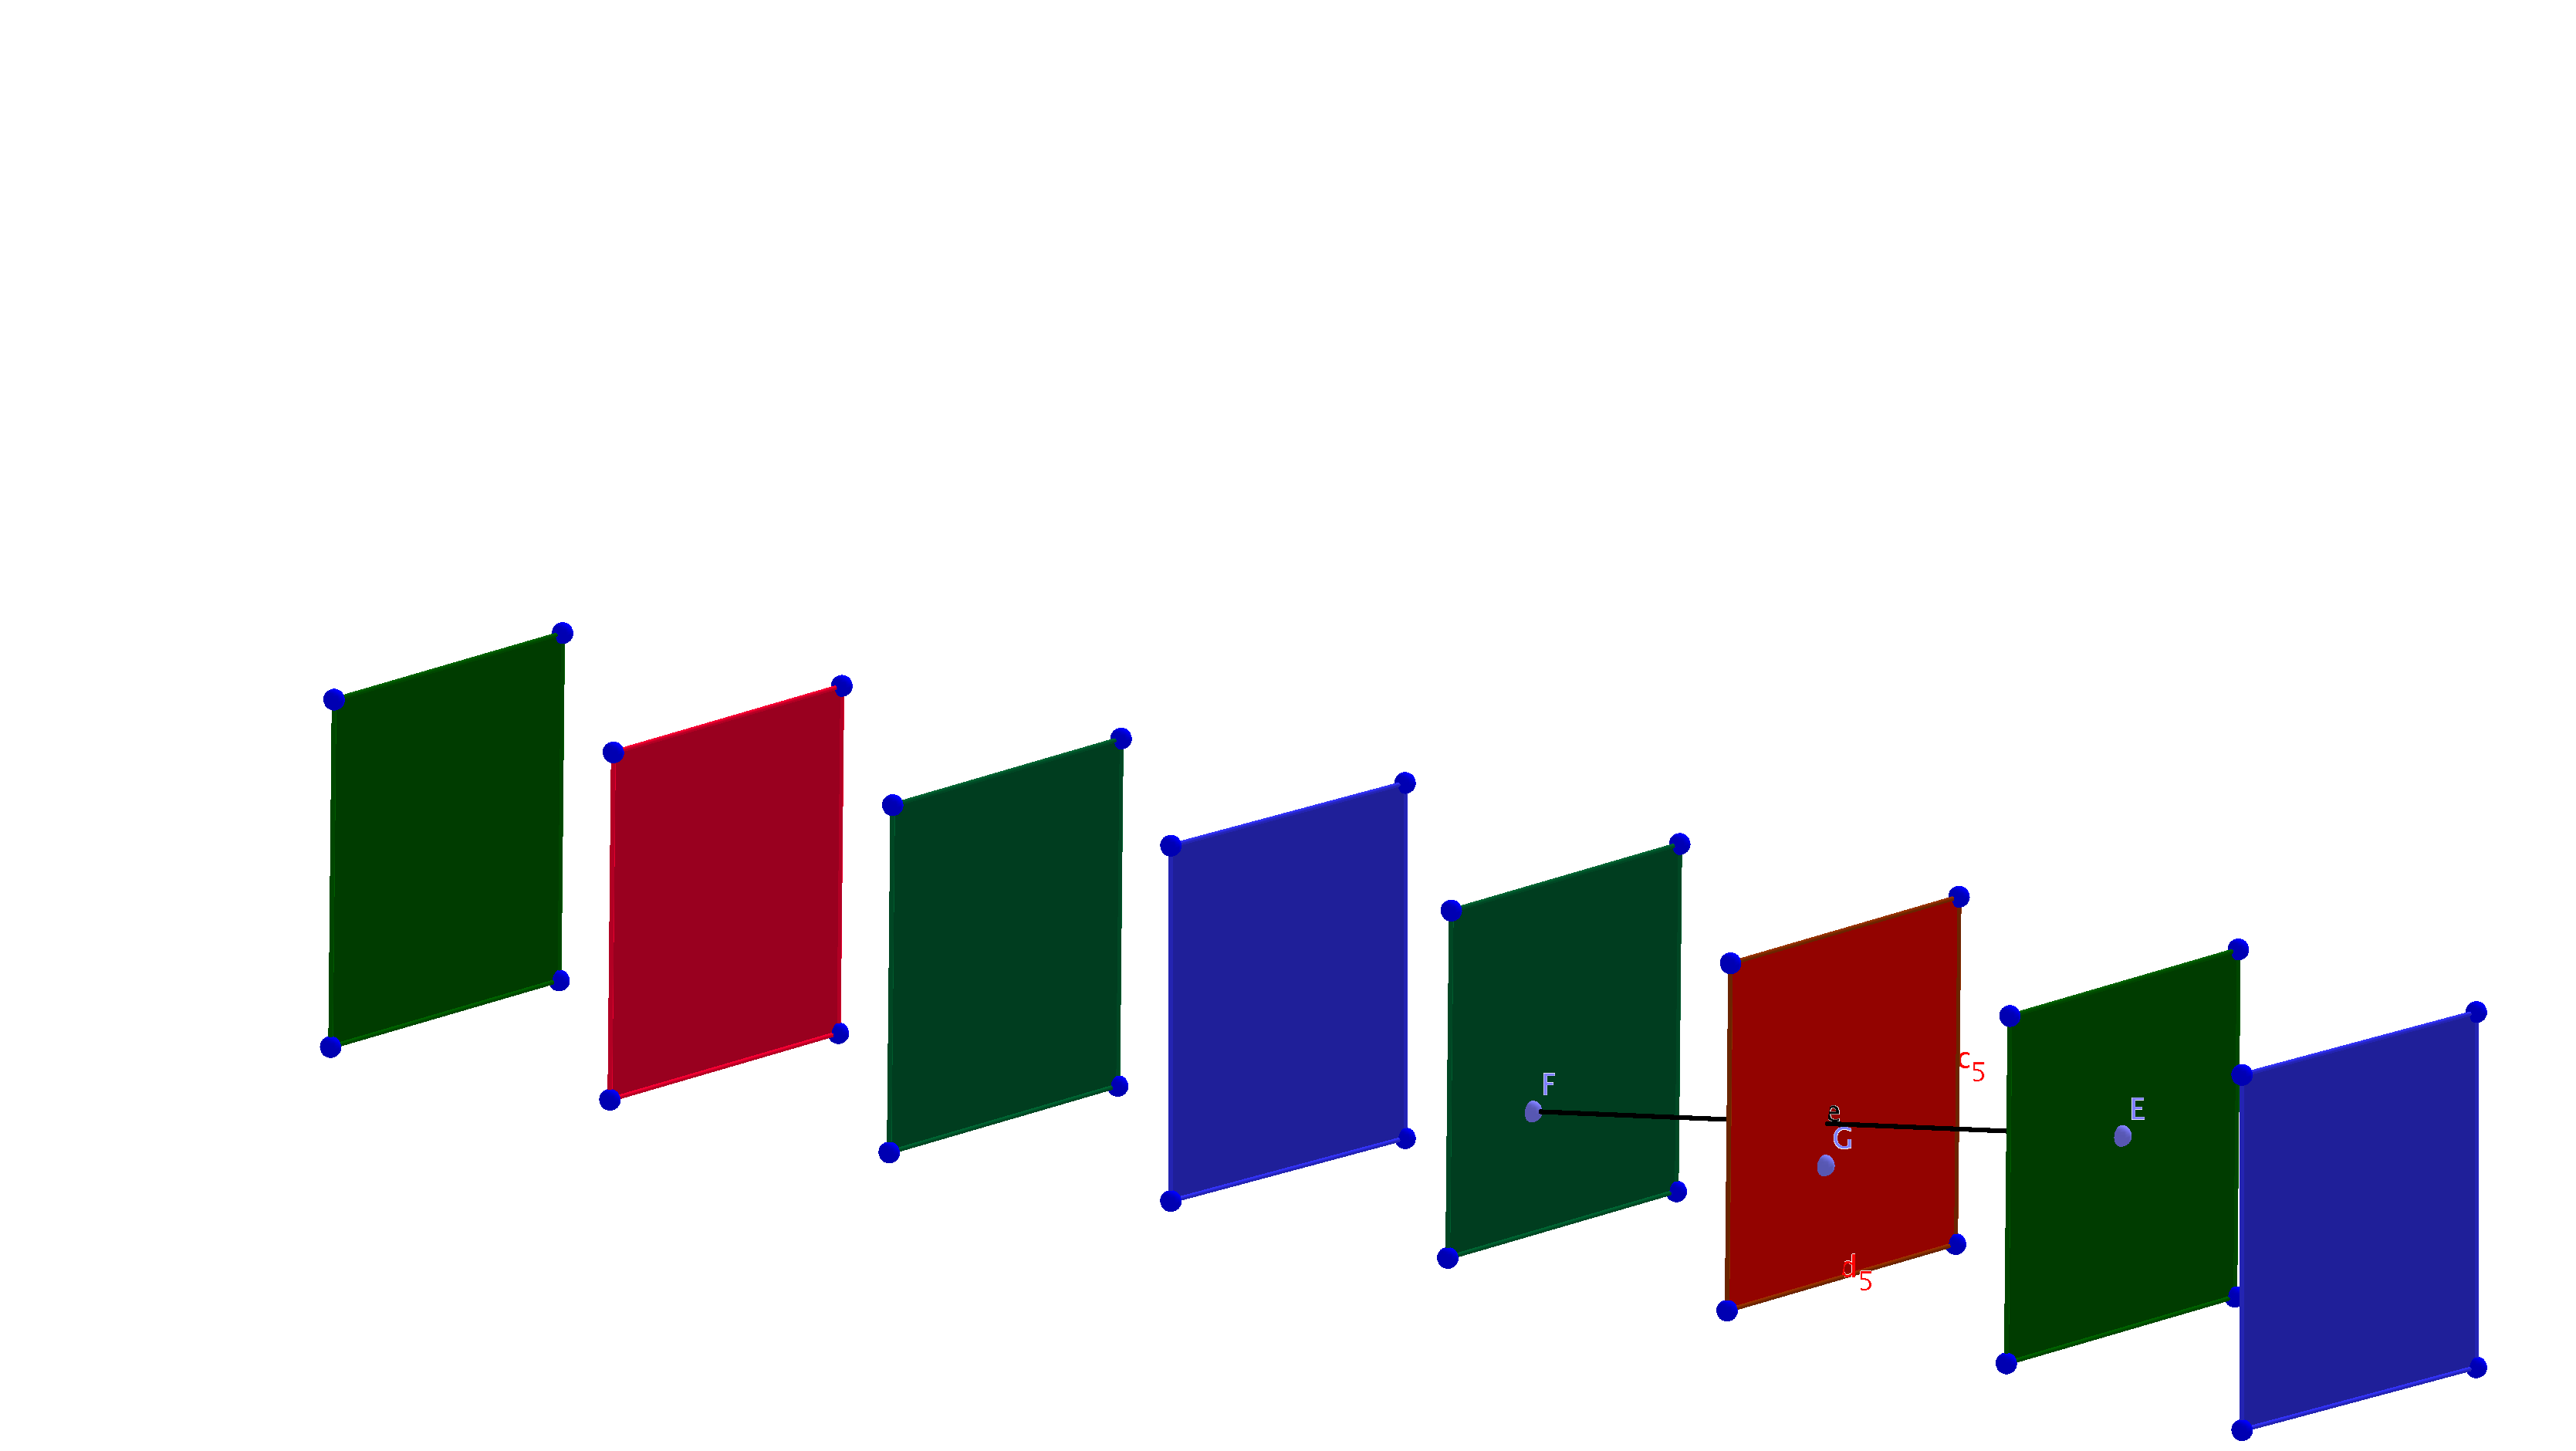
\includegraphics[width=1.0\linewidth]{figures/tripletDoubletFormed.png}
\caption{Doublet which has passed the DoubletDistCut used to look for a triplet. The green planes are used to create the doublets. The red plane with the green planes are used to create the triplets on each arm. The blue planes are DUTs. The blue points are hits.}
\label{fig:TripForm}
\end{figure}

\begin{figure}[H]
\centering
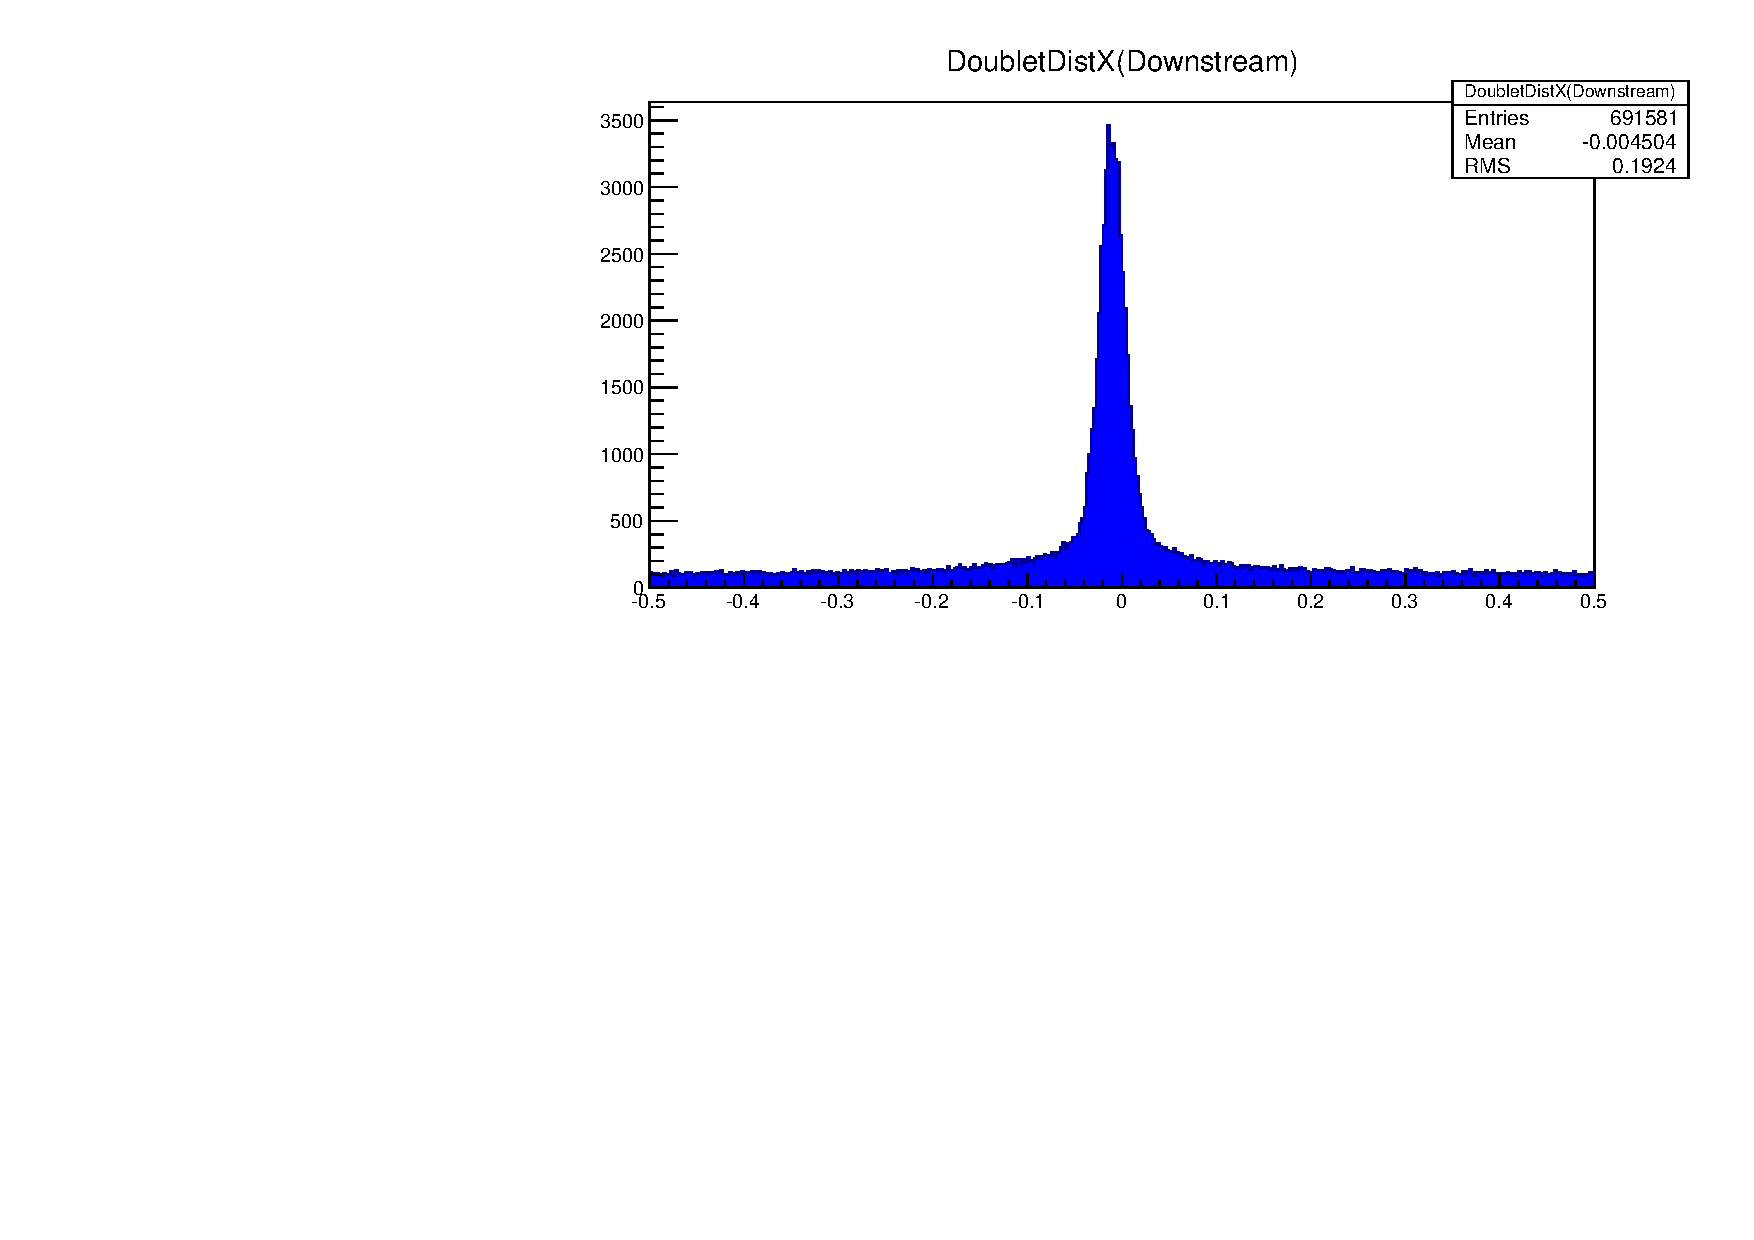
\includegraphics[width=1.0\linewidth]{figures/DoubletDistX-442-preOnly.pdf}
\caption{Doublet distance for down stream arm for DESY testbeam data taken at 4 GeV. This can be used to find the correct cuts for any setup.}
\label{fig:DoubDis}
\end{figure}

\item[DoubletCenDistCut]  The XY plane distance cut on the central planes (Red in figure \ref{fig:TripForm}) and prediction from doublet to create triplet . 

\begin{figure}[H]
\centering
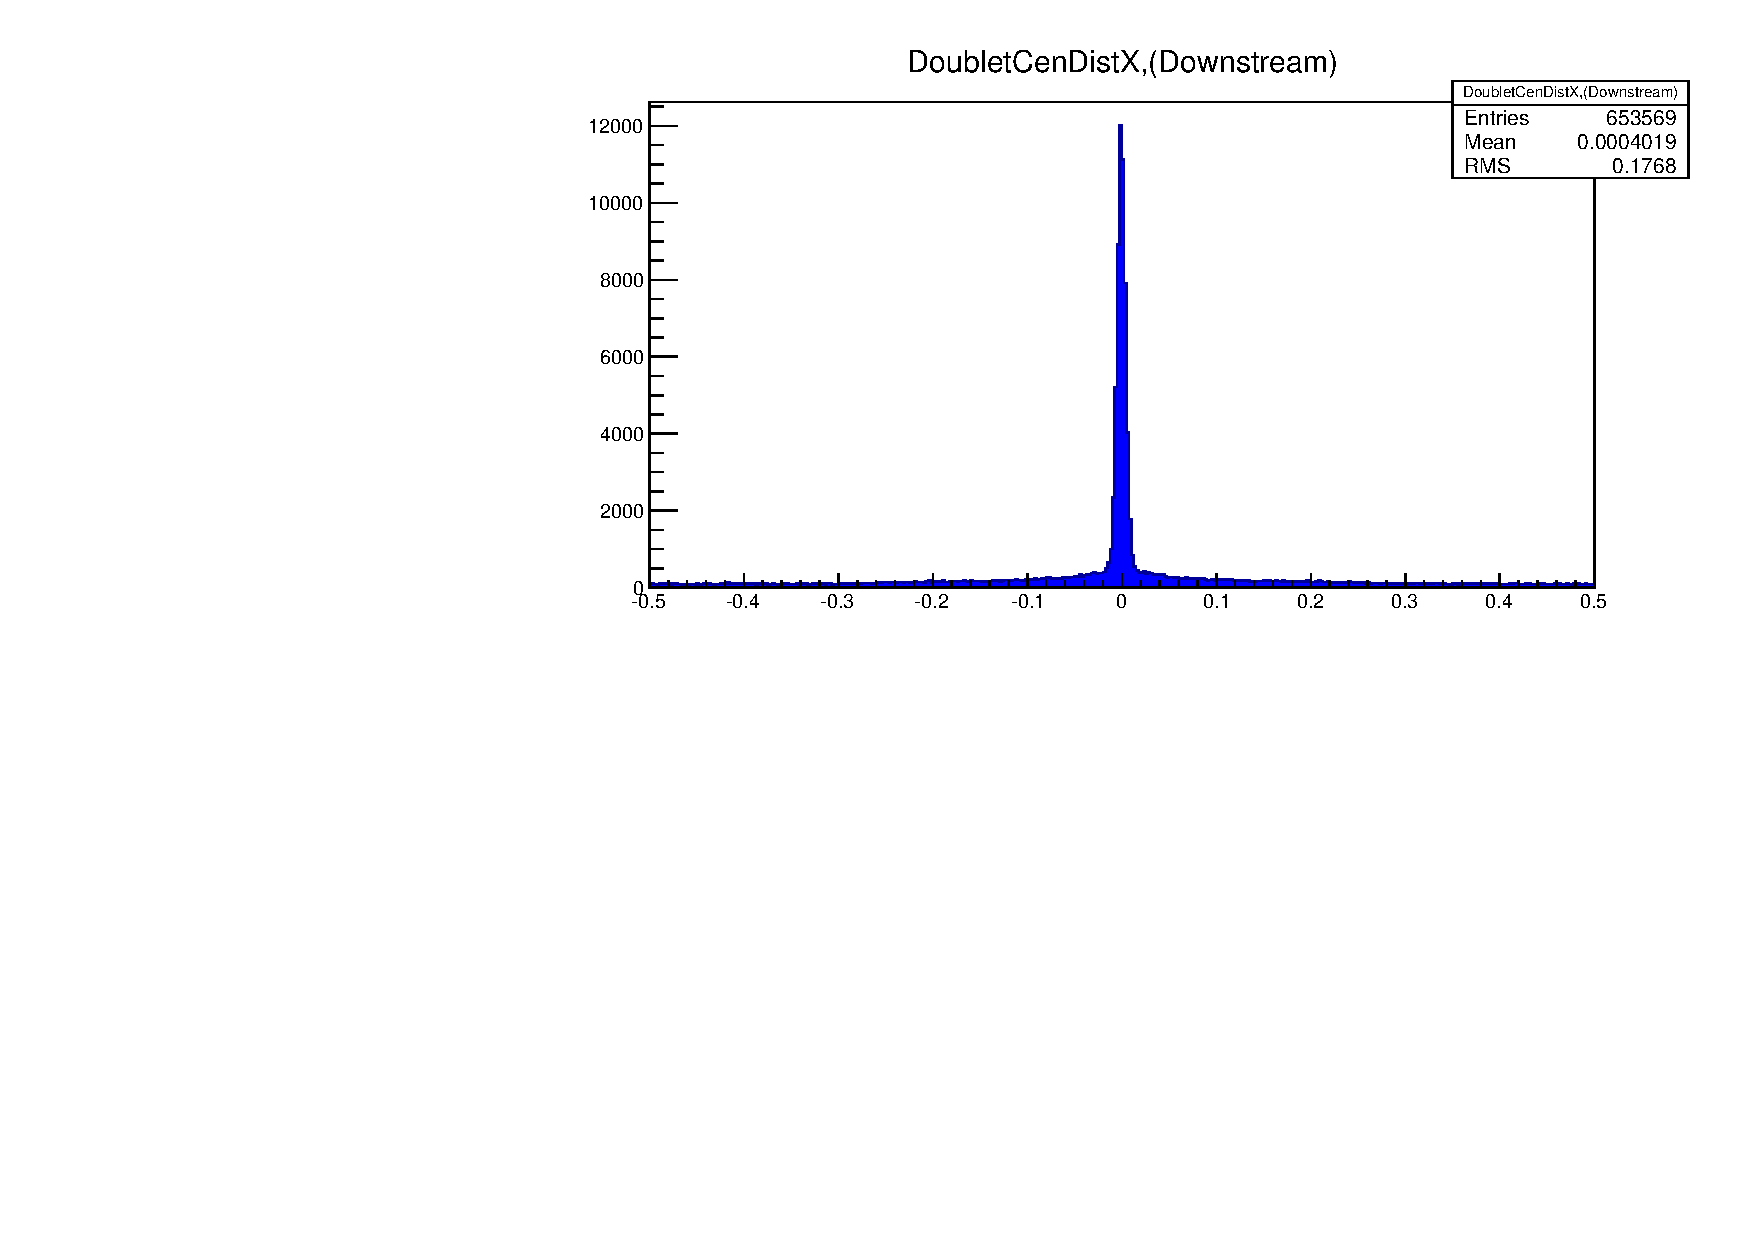
\includegraphics[width=1.0\linewidth]{figures/DoubletCenDist-442.pdf}
\caption{Doublet distance to central hit for down stream arm.}
\label{fig:DoubCen}
\end{figure}

\item[TripletConnectDistCut]  The triplets formed which pass the cuts are associated together using each triplet extrapolated to the centre of both triplets. With each triplet's position defined as the centre of of the doublet. This can be seen in figure \ref{fig:TripCon} were the triplets are extrapolated to a central point near the central DUT (DUTs in blue).

\begin{figure}[H]
\centering
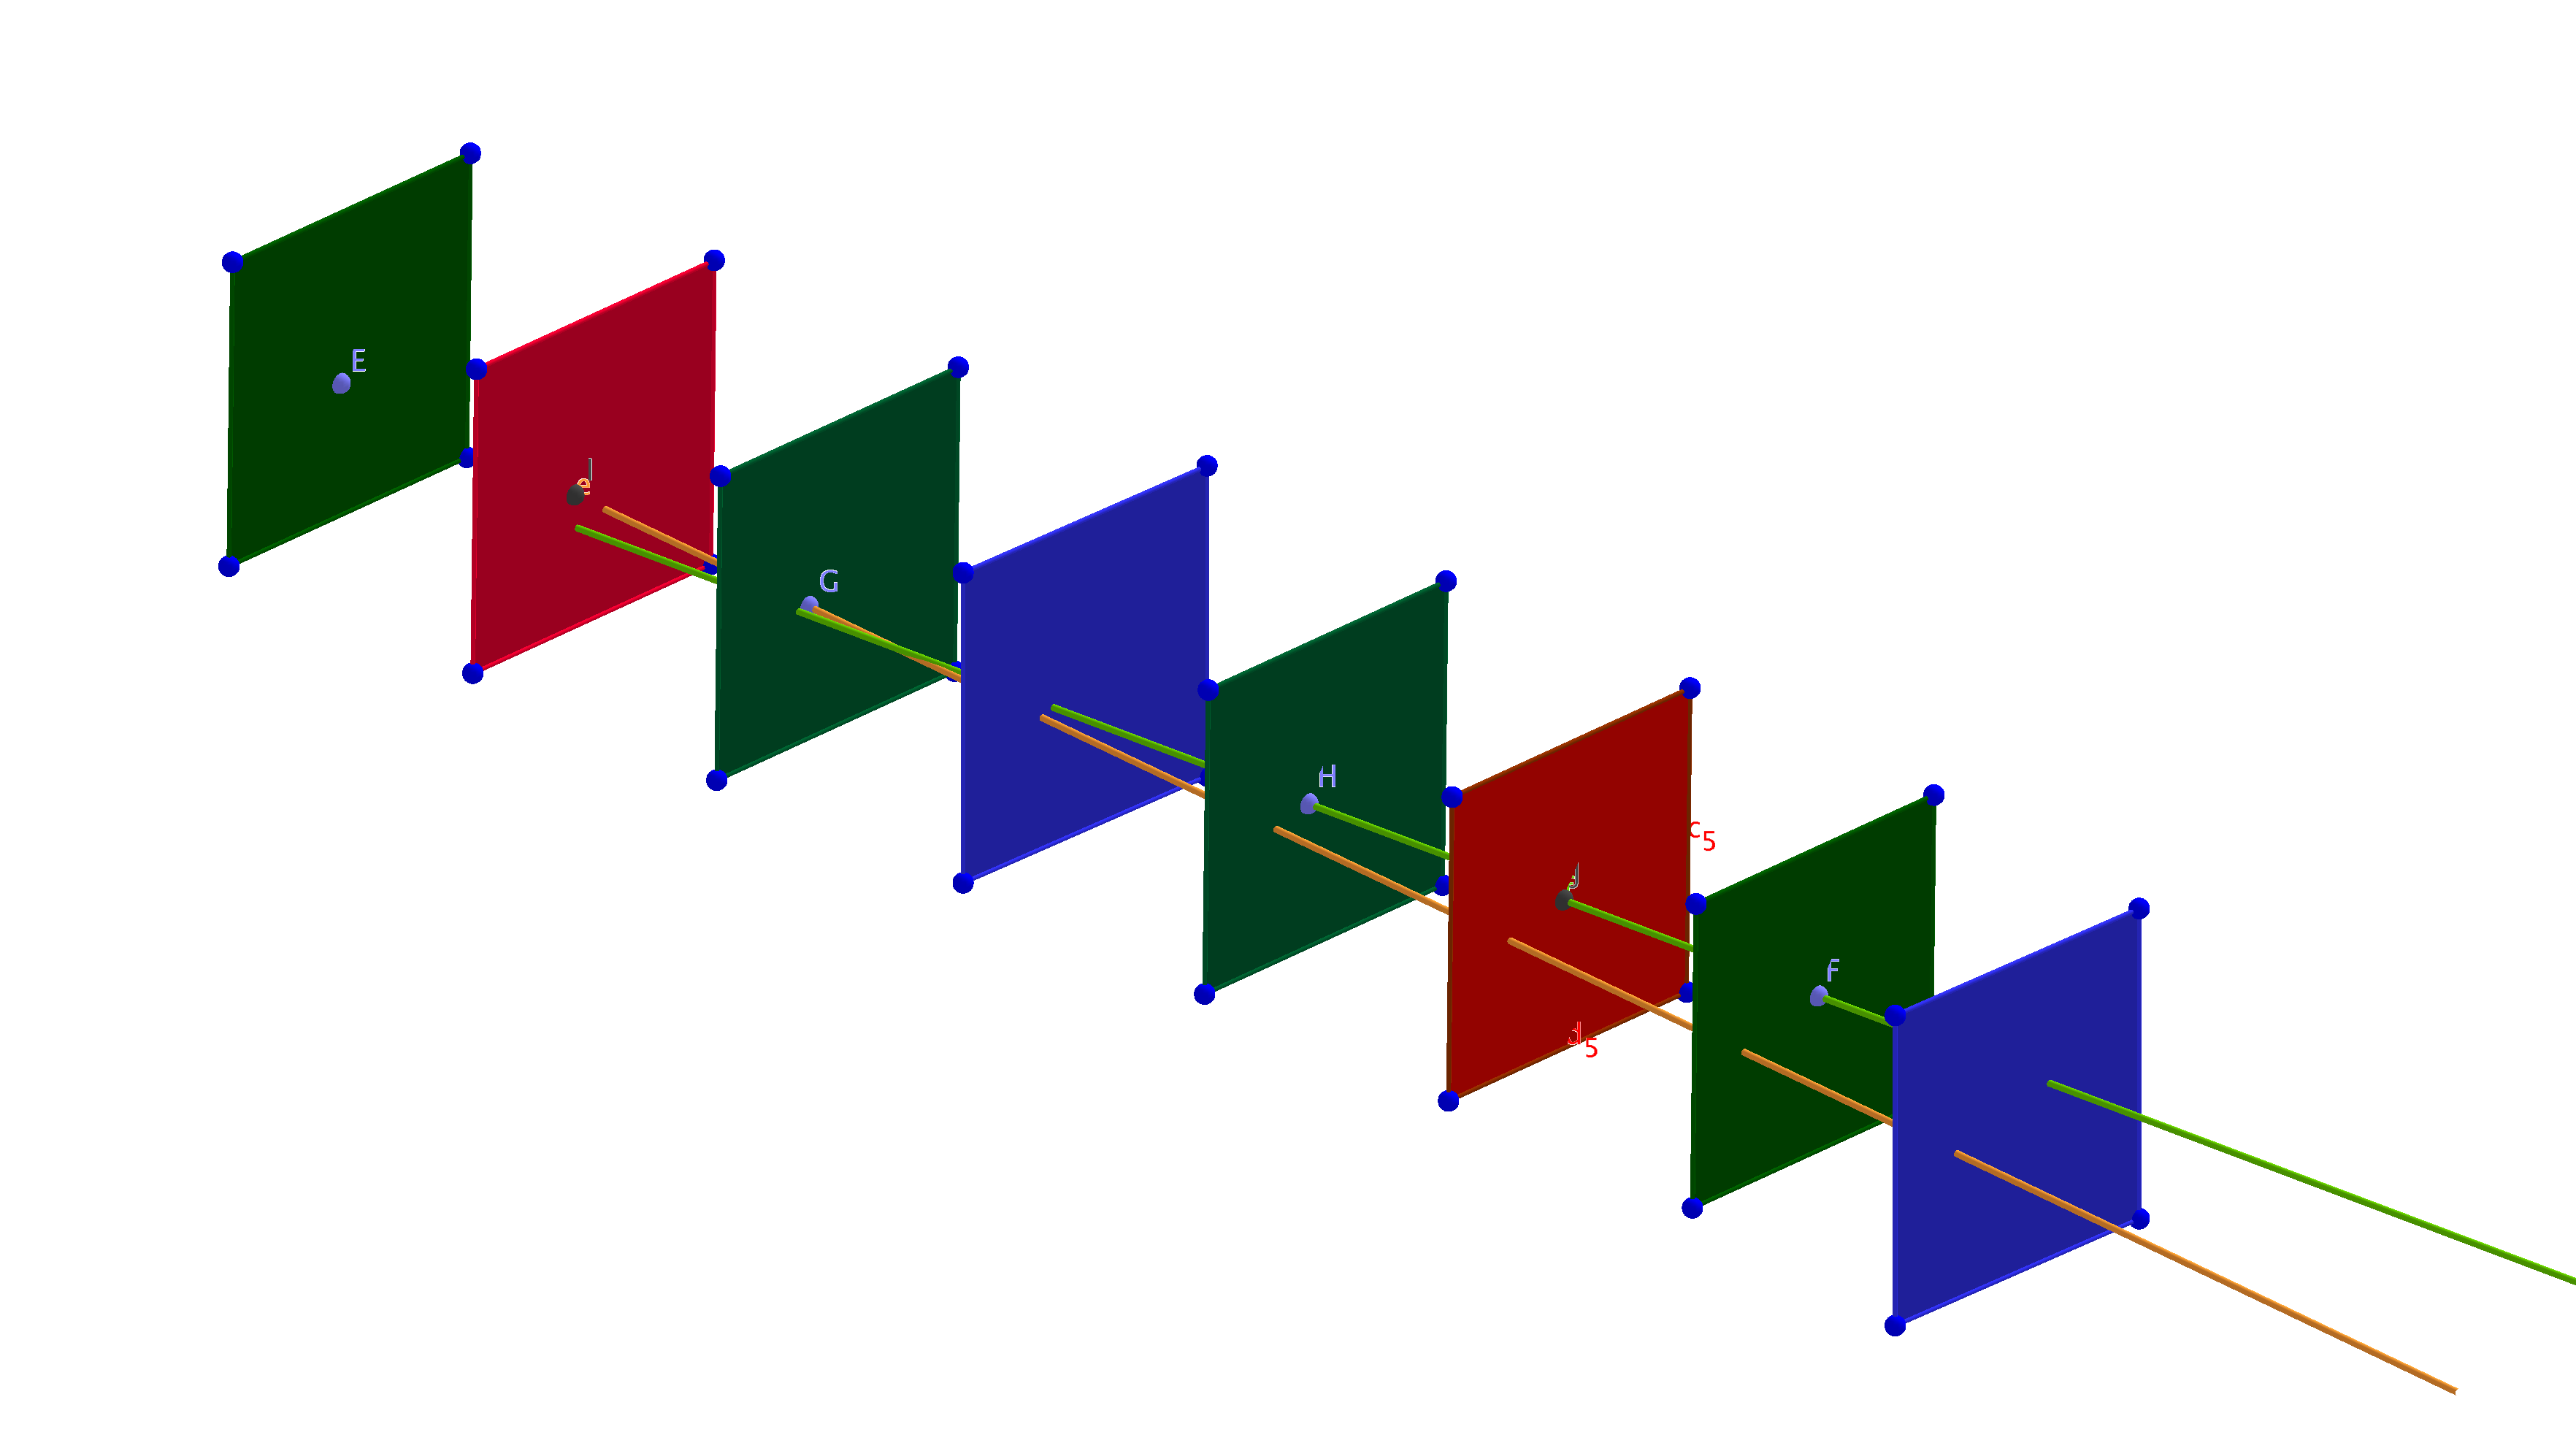
\includegraphics[width=1.0\linewidth]{figures/tripletsconnect.png}
\caption{A central point is used between both arms to compare both triplets' prediction. Each triplet is formed from the green and red planes of each arm. }
\label{fig:TripCon}
\end{figure}

\begin{figure}[H]
\centering
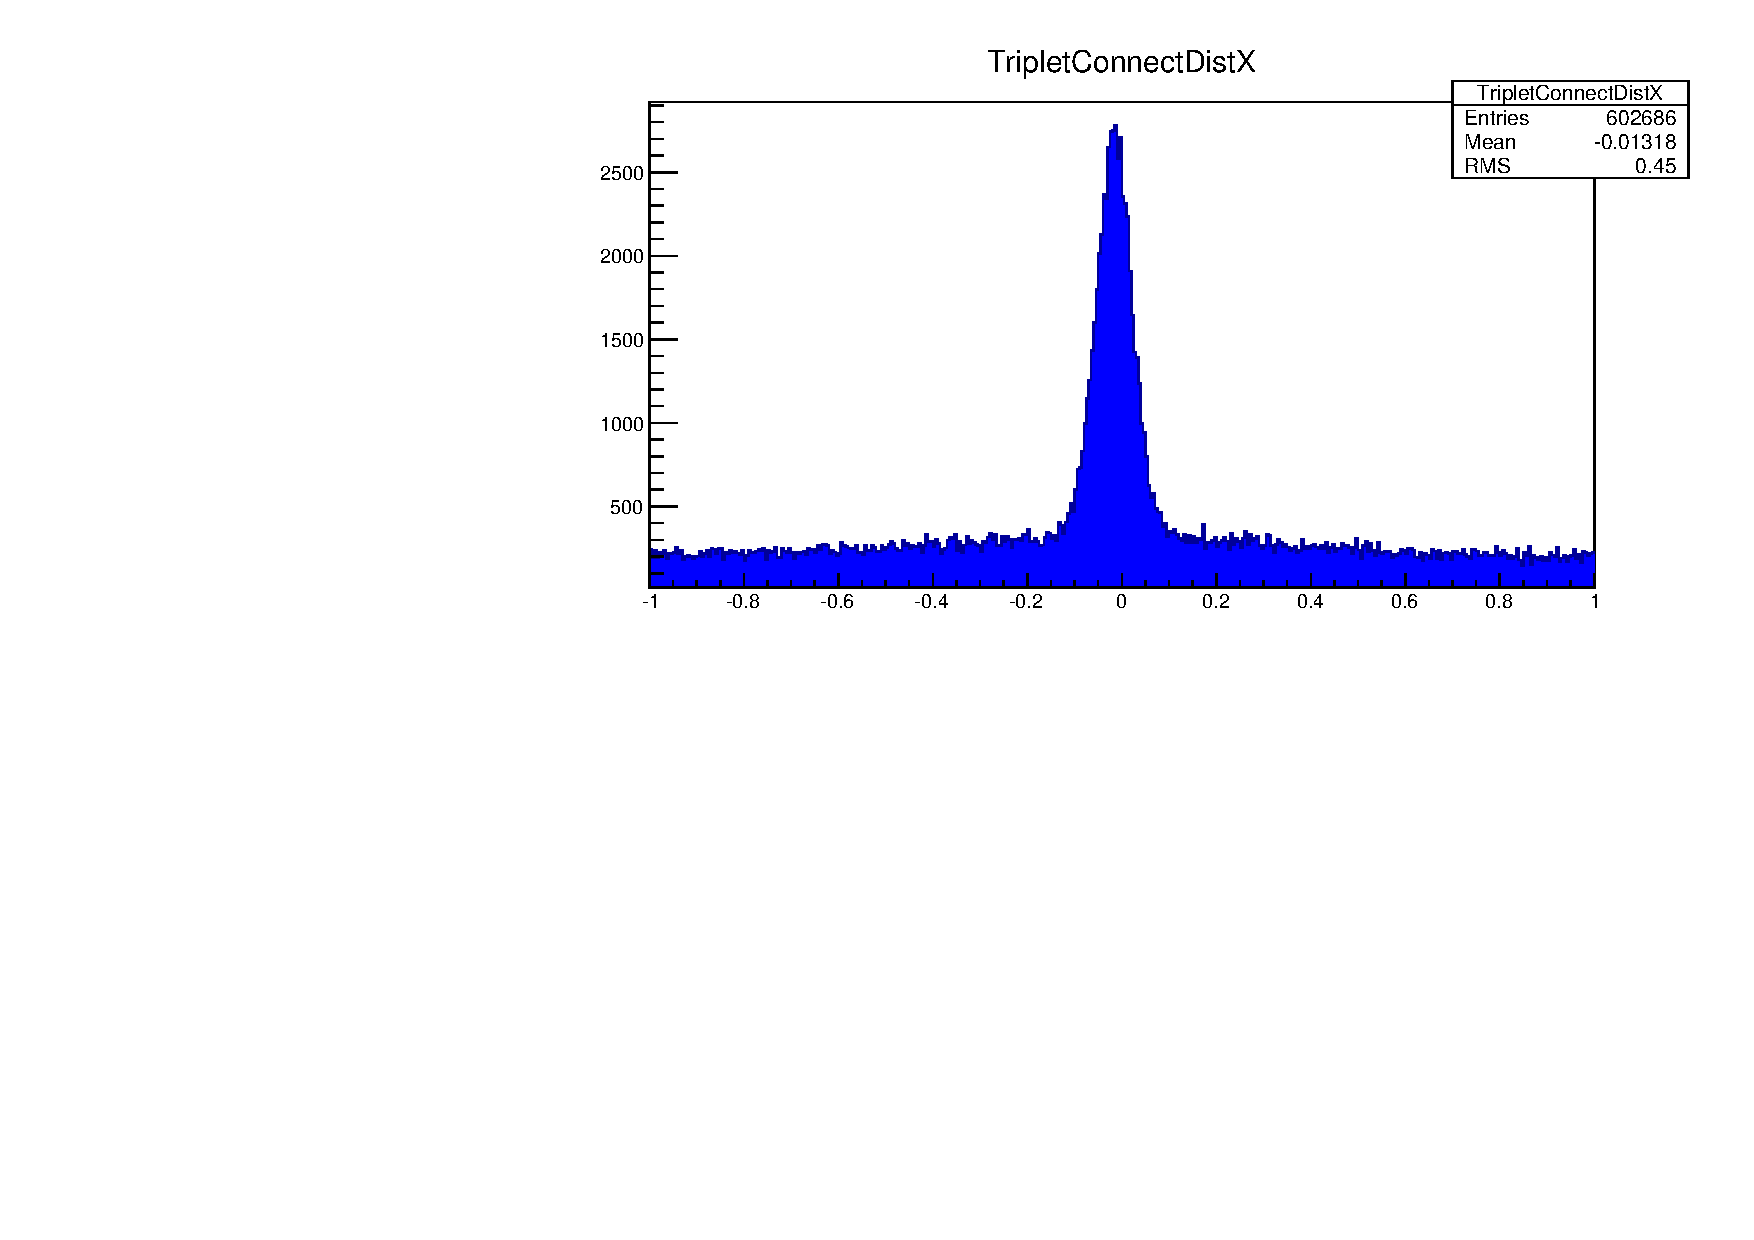
\includegraphics[width=1.0\linewidth]{figures/TripletConnectDistX-442.pdf}
\caption{The distance between the two triplet predictions at some central point.}
\label{fig:TripCen}
\end{figure}

\item[TripletSlopeCut] Figure \ref{fig:TripCon} shows that the prediction of both triplets can be accurate but the slope wrong. Therefore a slope cut between the two triplets must be applied. Testbeam setups in most cases only have a small beam divergence so this does not have to be precise.
\newline
\newline 
beam divergence = approx 1/0.5 mRad (DESY/SLAC)
\newline
\newline
The final track produced before the addition of DUT hits must come from a unique matching of triplets. If a triplet on one arm is matched with two triplets on the other then the triplet with two matches is removed.

\item[DUTWindow] After the triplets are associated together then the DUT hits are attached to this track if the hit is within some minimum distance. 
\begin{figure}[H]
\centering
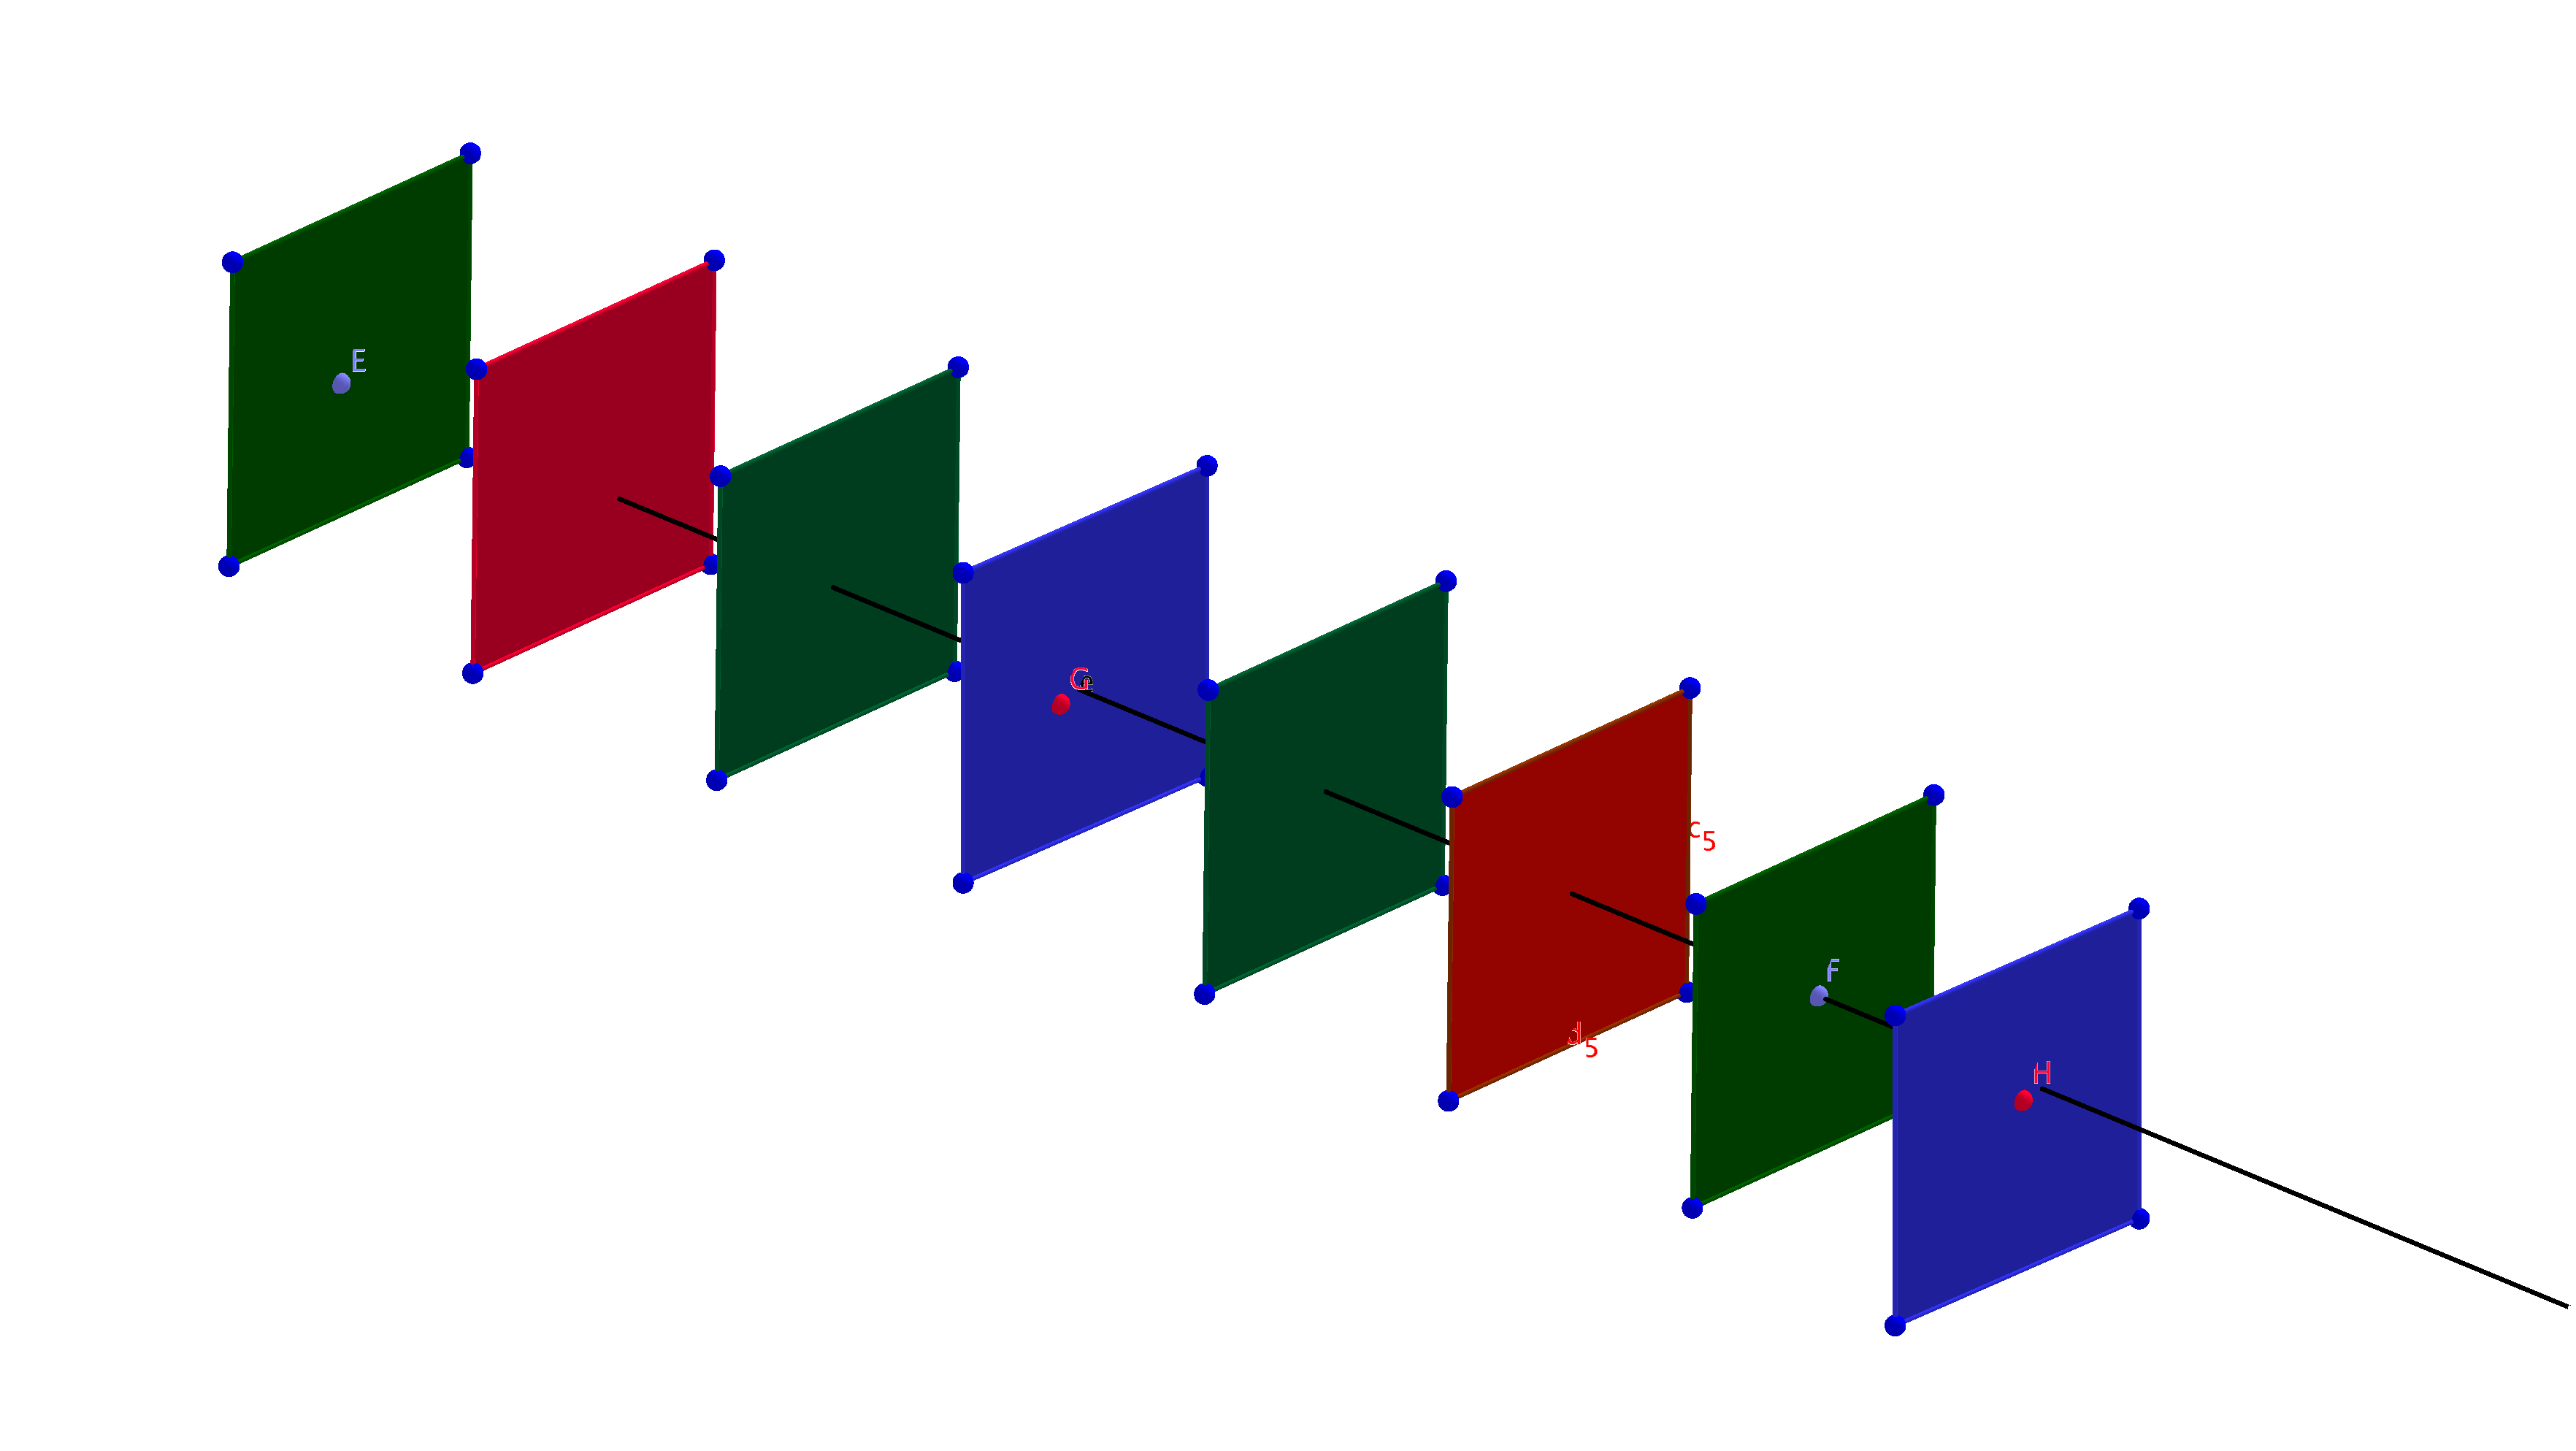
\includegraphics[width=1.0\linewidth]{figures/DUThitsPat.png}
\caption{The red dots on the blue DUT planes are hits. If the track produced by the mimosas is close to these hits then attach the hits to the track.}
\label{fig:DoubDis}
\end{figure}


\end{description}

Unique matching between a single DUT hit and a track must be found. If a track or hit is associated twice then the hit/track is removed from fitting with a DUT hit on that plane. All tracks produced by the mimosas are returned regardless of there being a DUT hit attached.

The hits collected which have been identified are assumed to come from a single track. How this track is described or parameterised depends on how accurate you want to be. Note parameterising is just the same as fitting, however to use the GBL algorithm you need an initial "guess". This initial guess must include positions, incidences, kink angles and curvature. The kink angles are fitted as parameters within GBL in contrast to many fitters which includes this as additional non diagonal variance in the propagated error matrix. In all examples this is not required and a single iteration of the GBL fitter with the basic internal parameterisation will suffice.

The information needed to use the GBL algorithm is the same of any track fitting method. Therefore the information provided here can be used with any fitting procedure. The only difference is the underlying "engine" which is used, in this case GBL. The construction of a track which can be used for alignment or analysis is done in five steps. The order does not pattern except the linking of trajectory points must be done before anything else. Each step will be covered in turn. 
\section{The five fold way}
\subsection{Linking trajectory points}
The initial requirement for track fitting is a coordinate system which links the local and global frames. The local frame is defined by the readout layout of the sensor, a Cartesian grid over the surface of the sensor and is unique for each DUT. The global frame is a Cartesian grid which extends over the full detector system. This is the same for all DUTs and alignment is needed to link both these frame for each DUT. Each plane is linked to the same global frame using the transformation:
\begin{equation}
 \overrightarrow{G} =   \hat{R}\overrightarrow{L} +  \overrightarrow{O}
\end{equation}

were the rotation matrix is defined

\begin{equation}
 \hat{R} = \hat{R_Y}\hat{R_X}\hat{R_Z}\hat{R_I}
\end{equation}

with $R_{X/Y/Z}$ as rotations in that particular axis. $R_I$ is the initial rotation matrix which can be set in gear to whatever value you see fit. The definition of these matrices come from TGeo manager and are documented online. Note the offsets are defined in the global frame since they are applied after all rotations. 

The order of applying transformations matters and must be considered. This is important for alignment and is discussed in section \ref{gloPar}. All large rotations round the X/Y axis must be applied as transforms to the initial matrix. If you apply this transform to $R_Y$/$R_X$ then the alignment matrix will not correspond to the correct frame for the rotation corrections. This can be ignored for rotations about 30 degrees. However if mapping between the local and global frame swaps axis then this is too large to adjust for and should be applied to the matrix $R_I$. The small changes to the rotations from alignment is applied to $\hat{R_Z}$,  $\hat{R_Y}$ and $\hat{R_X}$.


The full trajectory of a track does not need to be modeled for an accurate fit. Locations of high scattering and with measurements must be added. These points must be linked together using some Jacobian. A Jacobian in this case is just a link between how changes in position/incidence on one plane affects another. Curvature is an additional fitting term which is common to the track and does not vary with position. The Jacobian used to link the points together is 


\begin{center}
$
 \left( \begin{array}{cccccc}
1                            & 0       & 0        & 0 & 0  \\
\frac{F(0)ds}{dz} & 1        & 0        & 0 & 0  \\
\frac{F(1)ds}{dz} & 0        & 1        & 0 & 0  \\
0.5F(0)ds^2        & dz*ds & 0        & 1 & 0      \\  
0.5F(1)ds^2        & 0        & dz*ds & 0 &  1       \\  
  \label{eq:PC}
\end{array}
 \right)
$
\captionof{table}{The Jacobian used to link discrete points to form a continuous track. dz is the normalized direction of the track along z. ds is the arc length to the next point. F() is a vector which is the curvature of the track which depends on the energy and magnetic field the particle is immersed in.}
\end{center}

\begin{figure}[H]
\centering
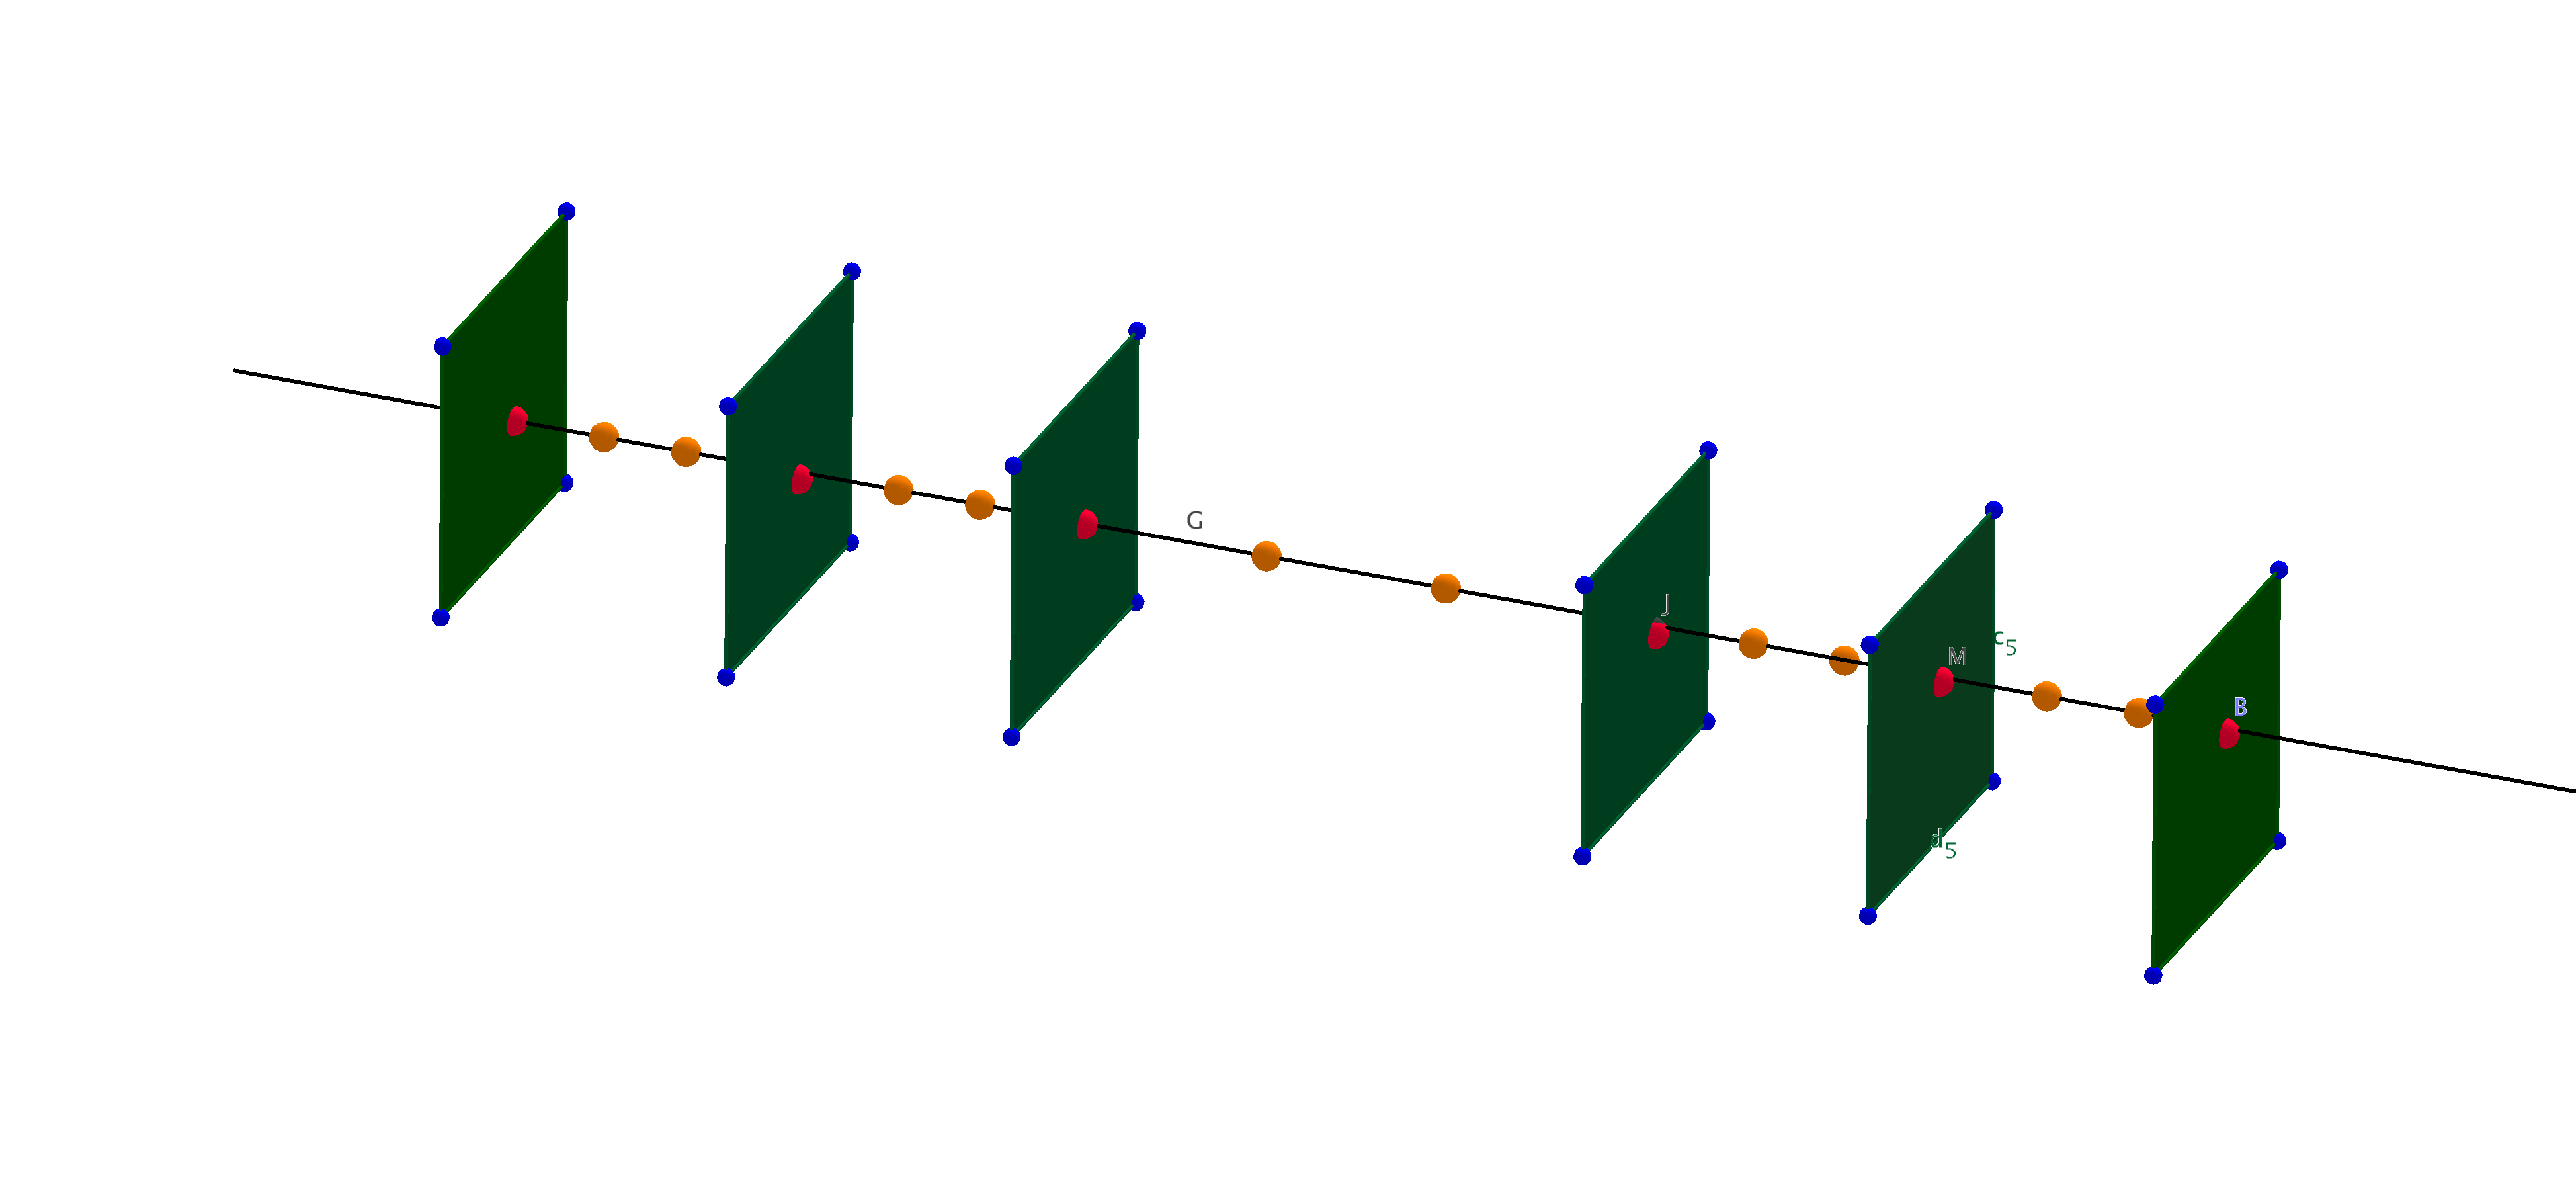
\includegraphics[width=1.0\linewidth]{figures/meas-scat-jac-link.png}
\caption{The red points have measurement and scattering information. The yellow points only scattering information. Measurements are the hit positions in the local frame. Scattering information is the kink angles measured in the local frame. Both have associated errors which must be determined. The Jacobian links all these point together so a change in one will affect a change in another.}
\label{fig:LinkJac}
\end{figure}


What points and where depend on the location of the measurement planes and the scattering from all the material. In the EUTelescope case a single point is used for each measurement and the material in front of this until the next measurement is associated with two points. Two points are need to describe a thick scatterer which is discussed in section \ref{sec:scat}. The linking of the full trajectory is done in the global frame.

\subsection{Add measurement information to points}

The measurements on the planes must be added to the trajectory created. The measurements are the residuals (Measured-Predicted) and the associated errors. The trajectory is always in the global frame and each measurement plane will not always be in this frame. Therefore propagation between the global and local frame is needed to link this information.
The propagation matrix used is

\[ 
\left( \begin{array}{ccc}
1  & 0   & -\frac{dx}{dz}   \\
0   & 1  & -\frac{dy}{dz}  
  \label{eq:prop}
\end{array}
 \right)
  \left( \begin{array}{cc}
 \overrightarrow{Rx}  &  \overrightarrow{Ry}  
\end{array}
 \right)
 \] 
 
 with slope defined in the local frame.  $\overrightarrow{Rx}$ and  $\overrightarrow{Ry}$ are the local X/Y axis defined in the global frame. The first matrix will transform the position from global to local frame. You only need to apply the partial rotation matrix since there should be no z displacement in this frame. The second part will determine the intersection on the XY plane in the local frame from a track propagated to the new local position.
 
 \begin{figure}[H]
\centering
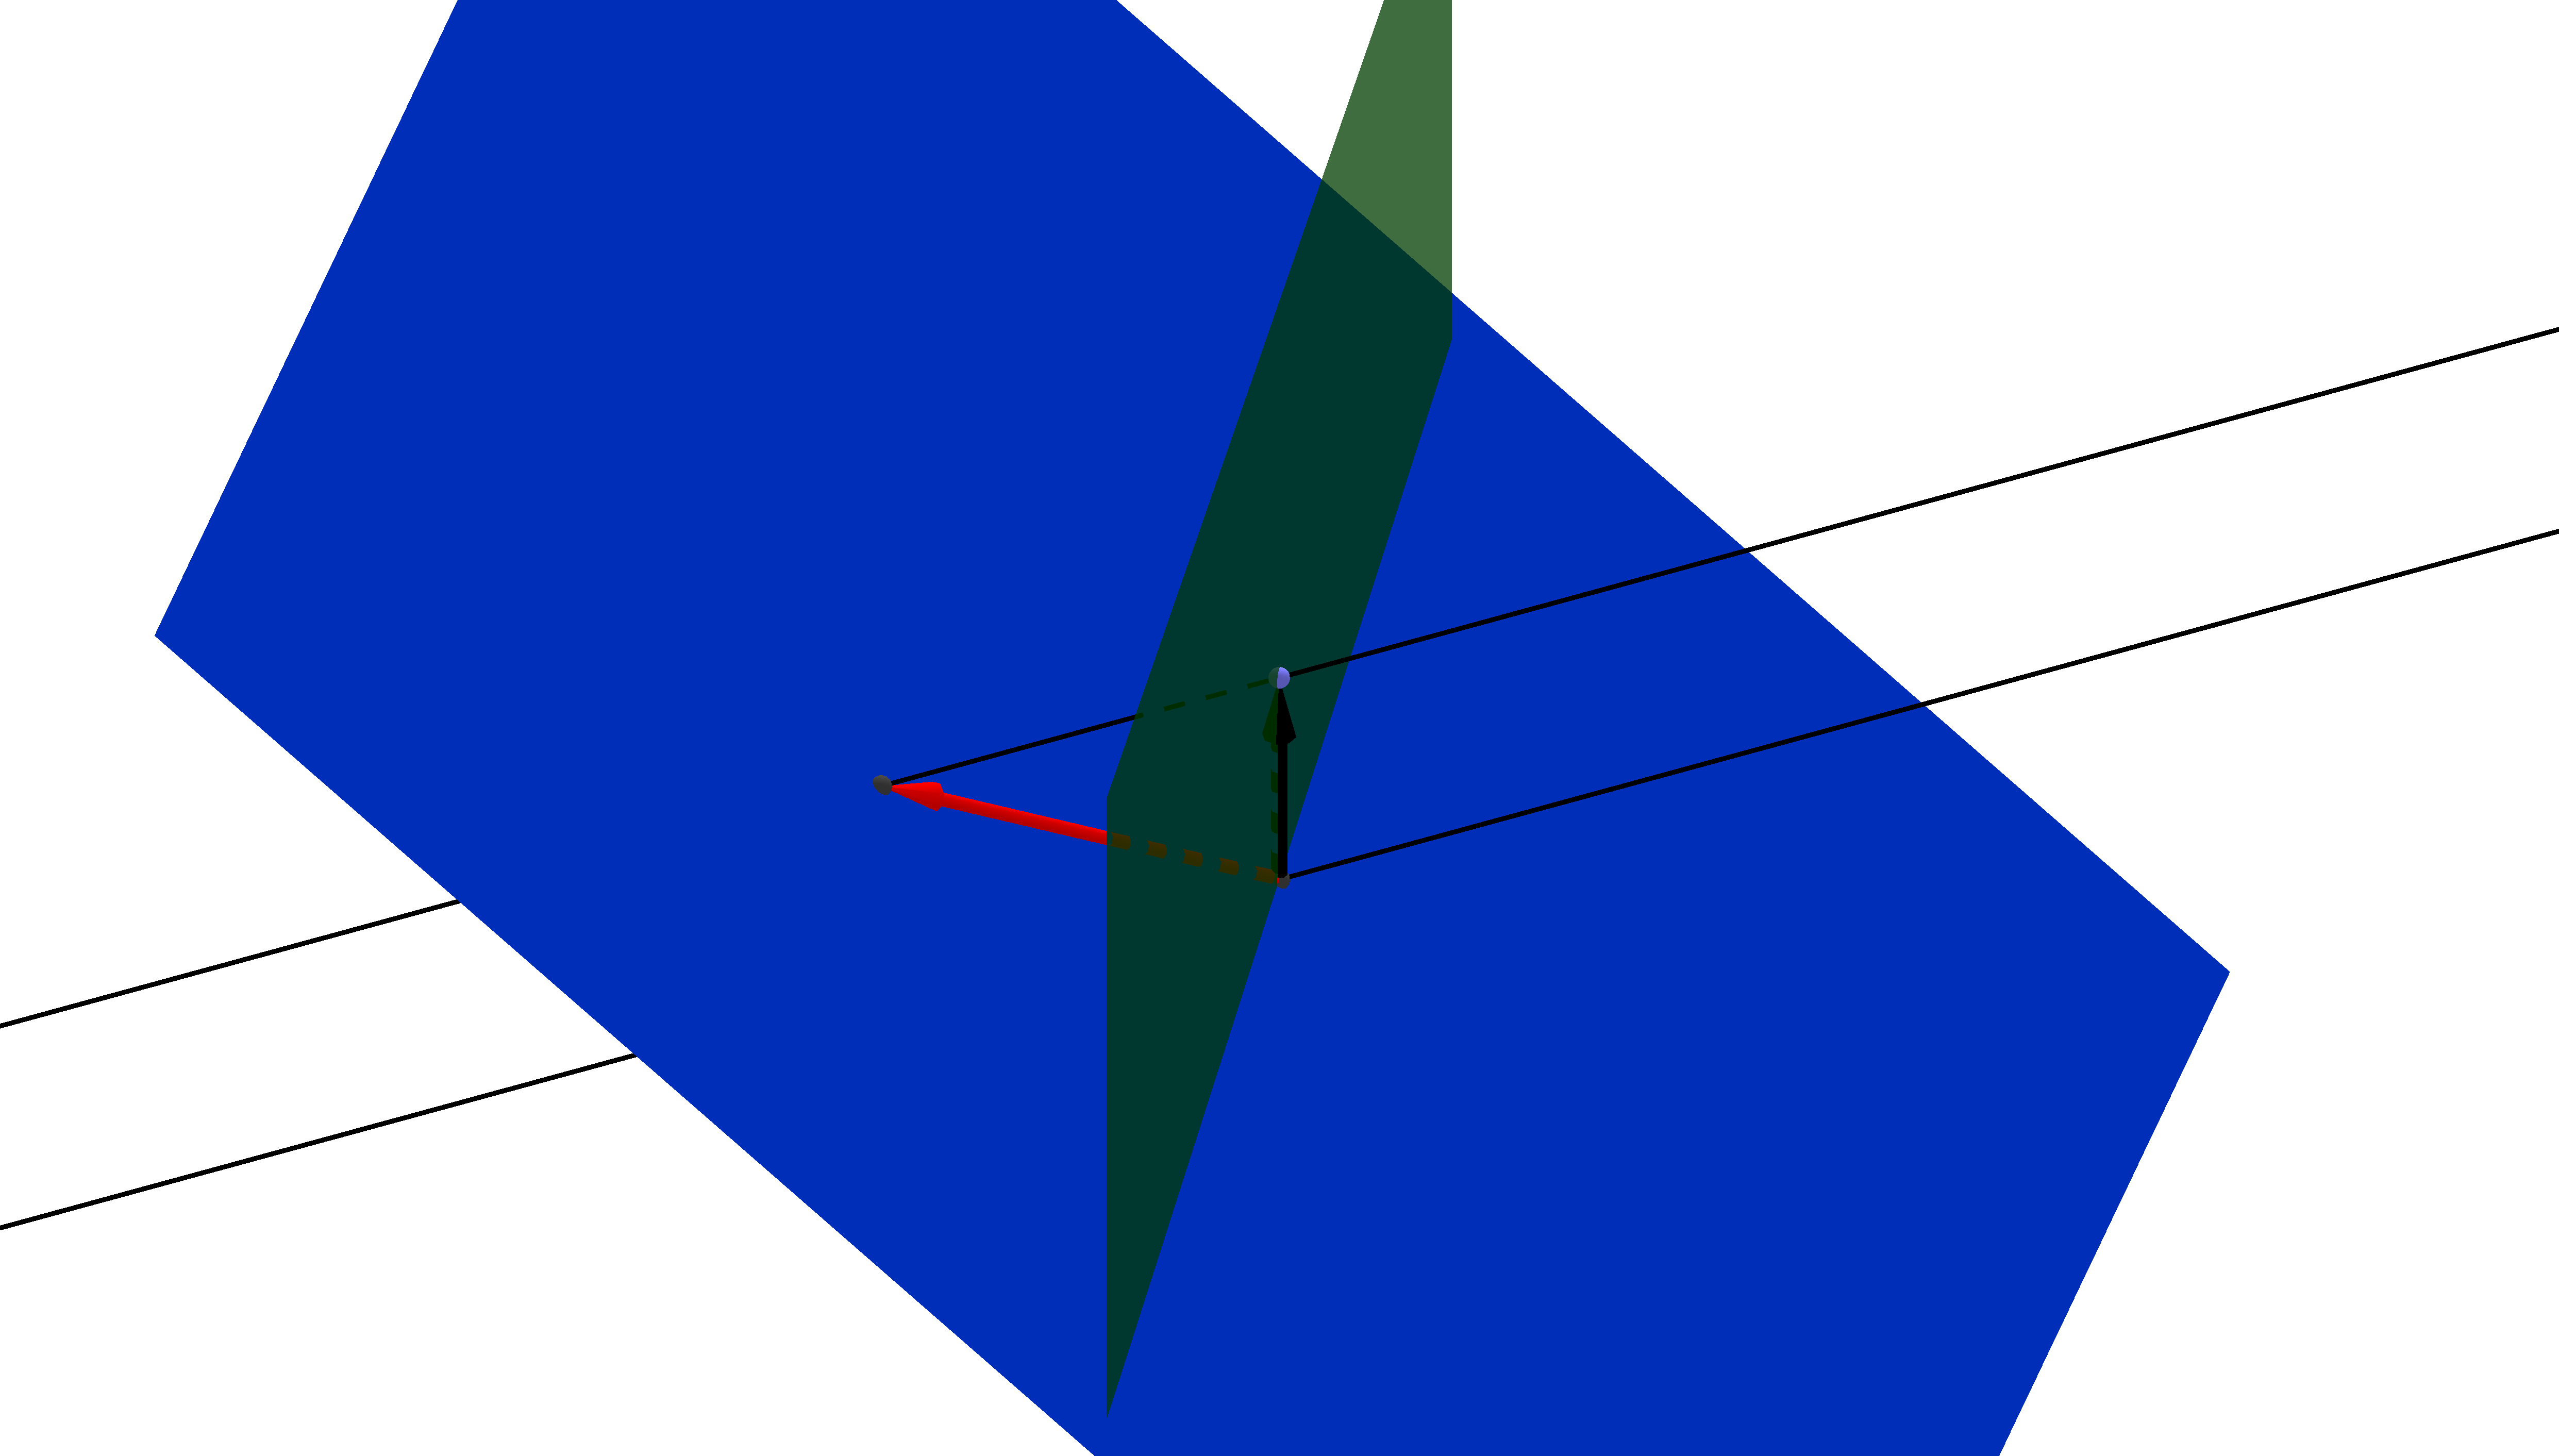
\includegraphics[width=1.0\linewidth]{figures/prop.png}
\caption{The projection matrix will relate the change in residual (black vector) in global XY plane to local XY plane (Blue plane). The propagation must take into account the change in track position intersection. The black lines are the track propagated to the new position.}
\label{fig:Prop}
\end{figure}
 
GBL expects a link which goes from global to local and this defines the parameters used above. You can define the slopes in the local frame and axis in global frame and then invert the corresponding matrix. Either or will work.

The errors associated in the local frame need not be diagonal and will be transformed internally to a frame in which they are. However they must be correct for each measurement. This is simple in most cases were each measurement is independent of position in the local frame. This is true for most strip and pixel sensors but not all. A simple example being a strip sensor with radial strips. This would require that each position has a different error matrix associated with it. Since each strip is oriented differently to the local Cartesian grid which defines the local frame. This situation highlights the difference between the local frame and measurement frame which is often discussed in literature. The measurement frame in one in which the errors are diagonal. Therefore for this example each strips orientation would require a different measurement frame. This requirement has been considered and can be easily added to the measurement function which adds this information.



\subsection{Add scattering information}
\label{sec:scat}
Scattering in the EUTelescope framework is always assumed to be thin (Discussed later). Furthermore the scattering error will non be diagonal in the local frame of the sensor. The propagation matrix from the frame parallel to the track and local frame is

\[ 
\frac{\theta_{0}^{2}}{1-c^2_1 c^2_2}
\left(
  \begin{array}{cc}
 1-c^{2}_{2} & c_{1}c_{2}    \\
 c_{1}c_{2} & 1-c^{2}_{1} \\   
\end{array} \right)\] 



This propagation is shown by \ref{fig:ScatFrame} with the plane perpendicular to the track containing the diagonal error matrix. However if the matrix is transformed to the plane frame (Blue plane \ref{fig:ScatFrame}) then the error matrix will be non diagonal.

\begin{figure}[H]
\centering
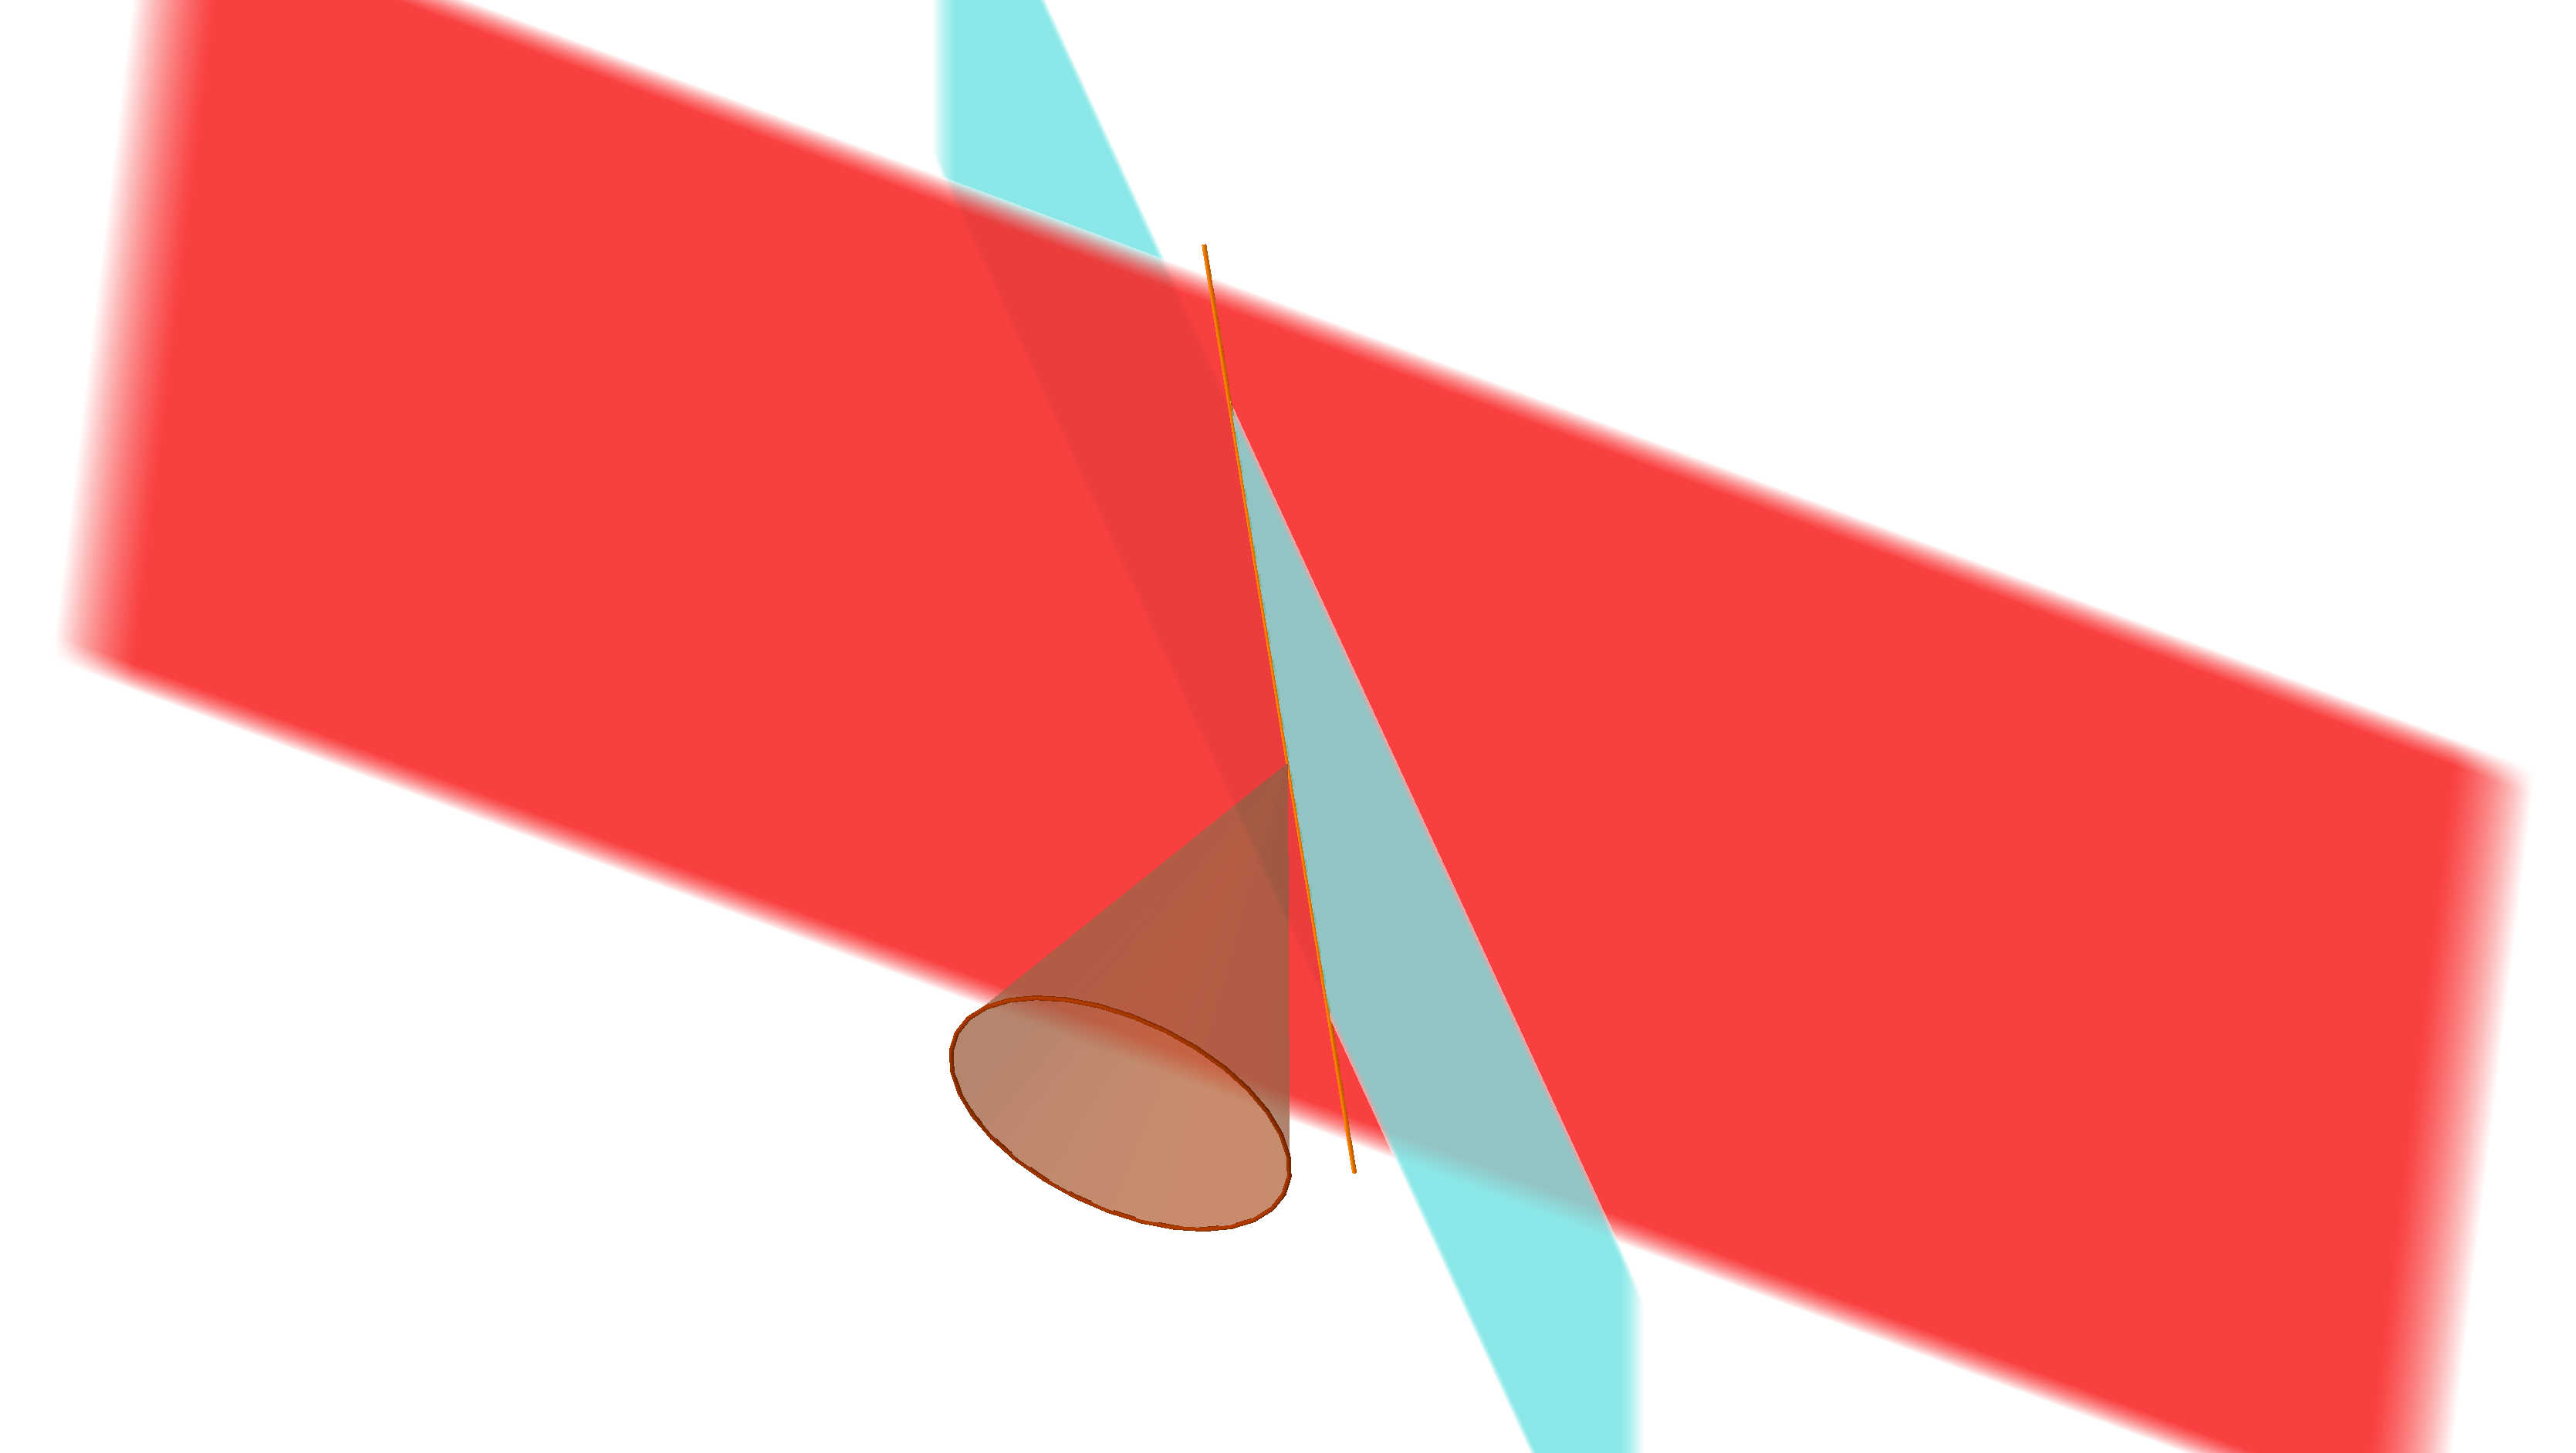
\includegraphics[width=1.0\linewidth]{figures/propGood600.png}
\caption{The scattering frame is the red plane which is perpendicular to the track. The blue plane is the sensor surface. Compare the circular cone which has a diagonal error matrix to the ellipsoid which is non diagonal. This ellipsoid is better seen if the XY plane is propagated downstream with the errors \ref{fig:ScatFrame1}.}
\label{fig:ScatFrame}
\end{figure}

The view of the errors associated from scattering on the plane is shown in figures \ref{fig:ScatFrame1} and \ref{fig:ScatFrame2}. 

\begin{figure}[H]
\centering
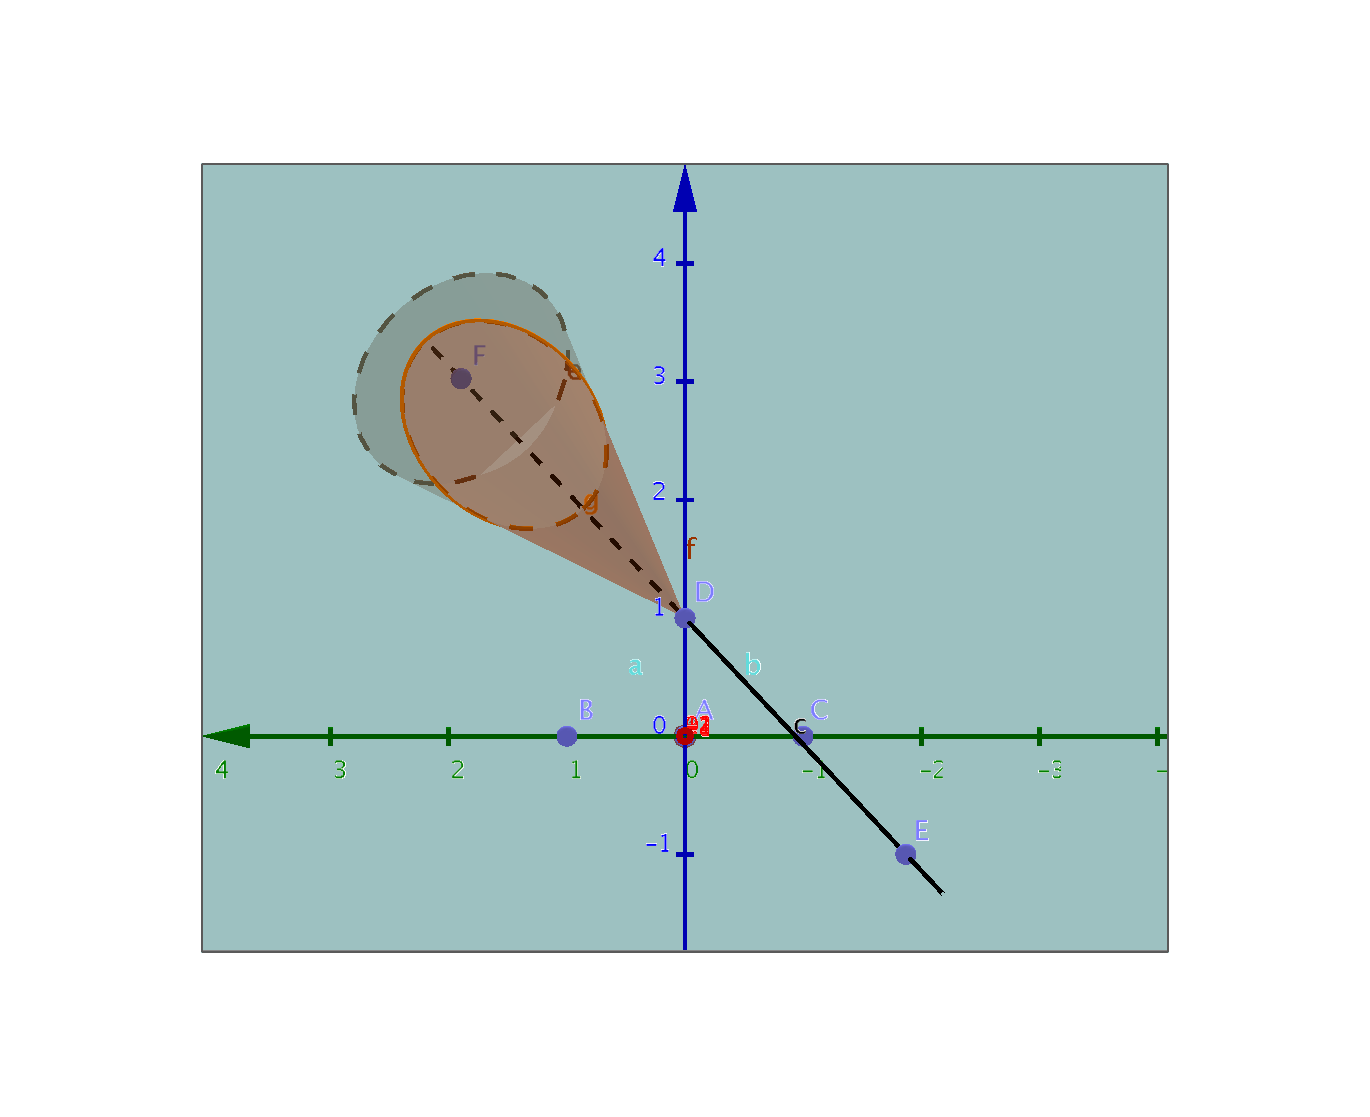
\includegraphics[width=1.0\linewidth]{figures/scatterDownZProjection.png}
\caption{The scattering cone projected on the XY plane of the sensor. The errors on the sensor must take this form to propagate correctly in the z axis}
\label{fig:ScatFrame1}
\end{figure}

\begin{figure}[H]
\centering
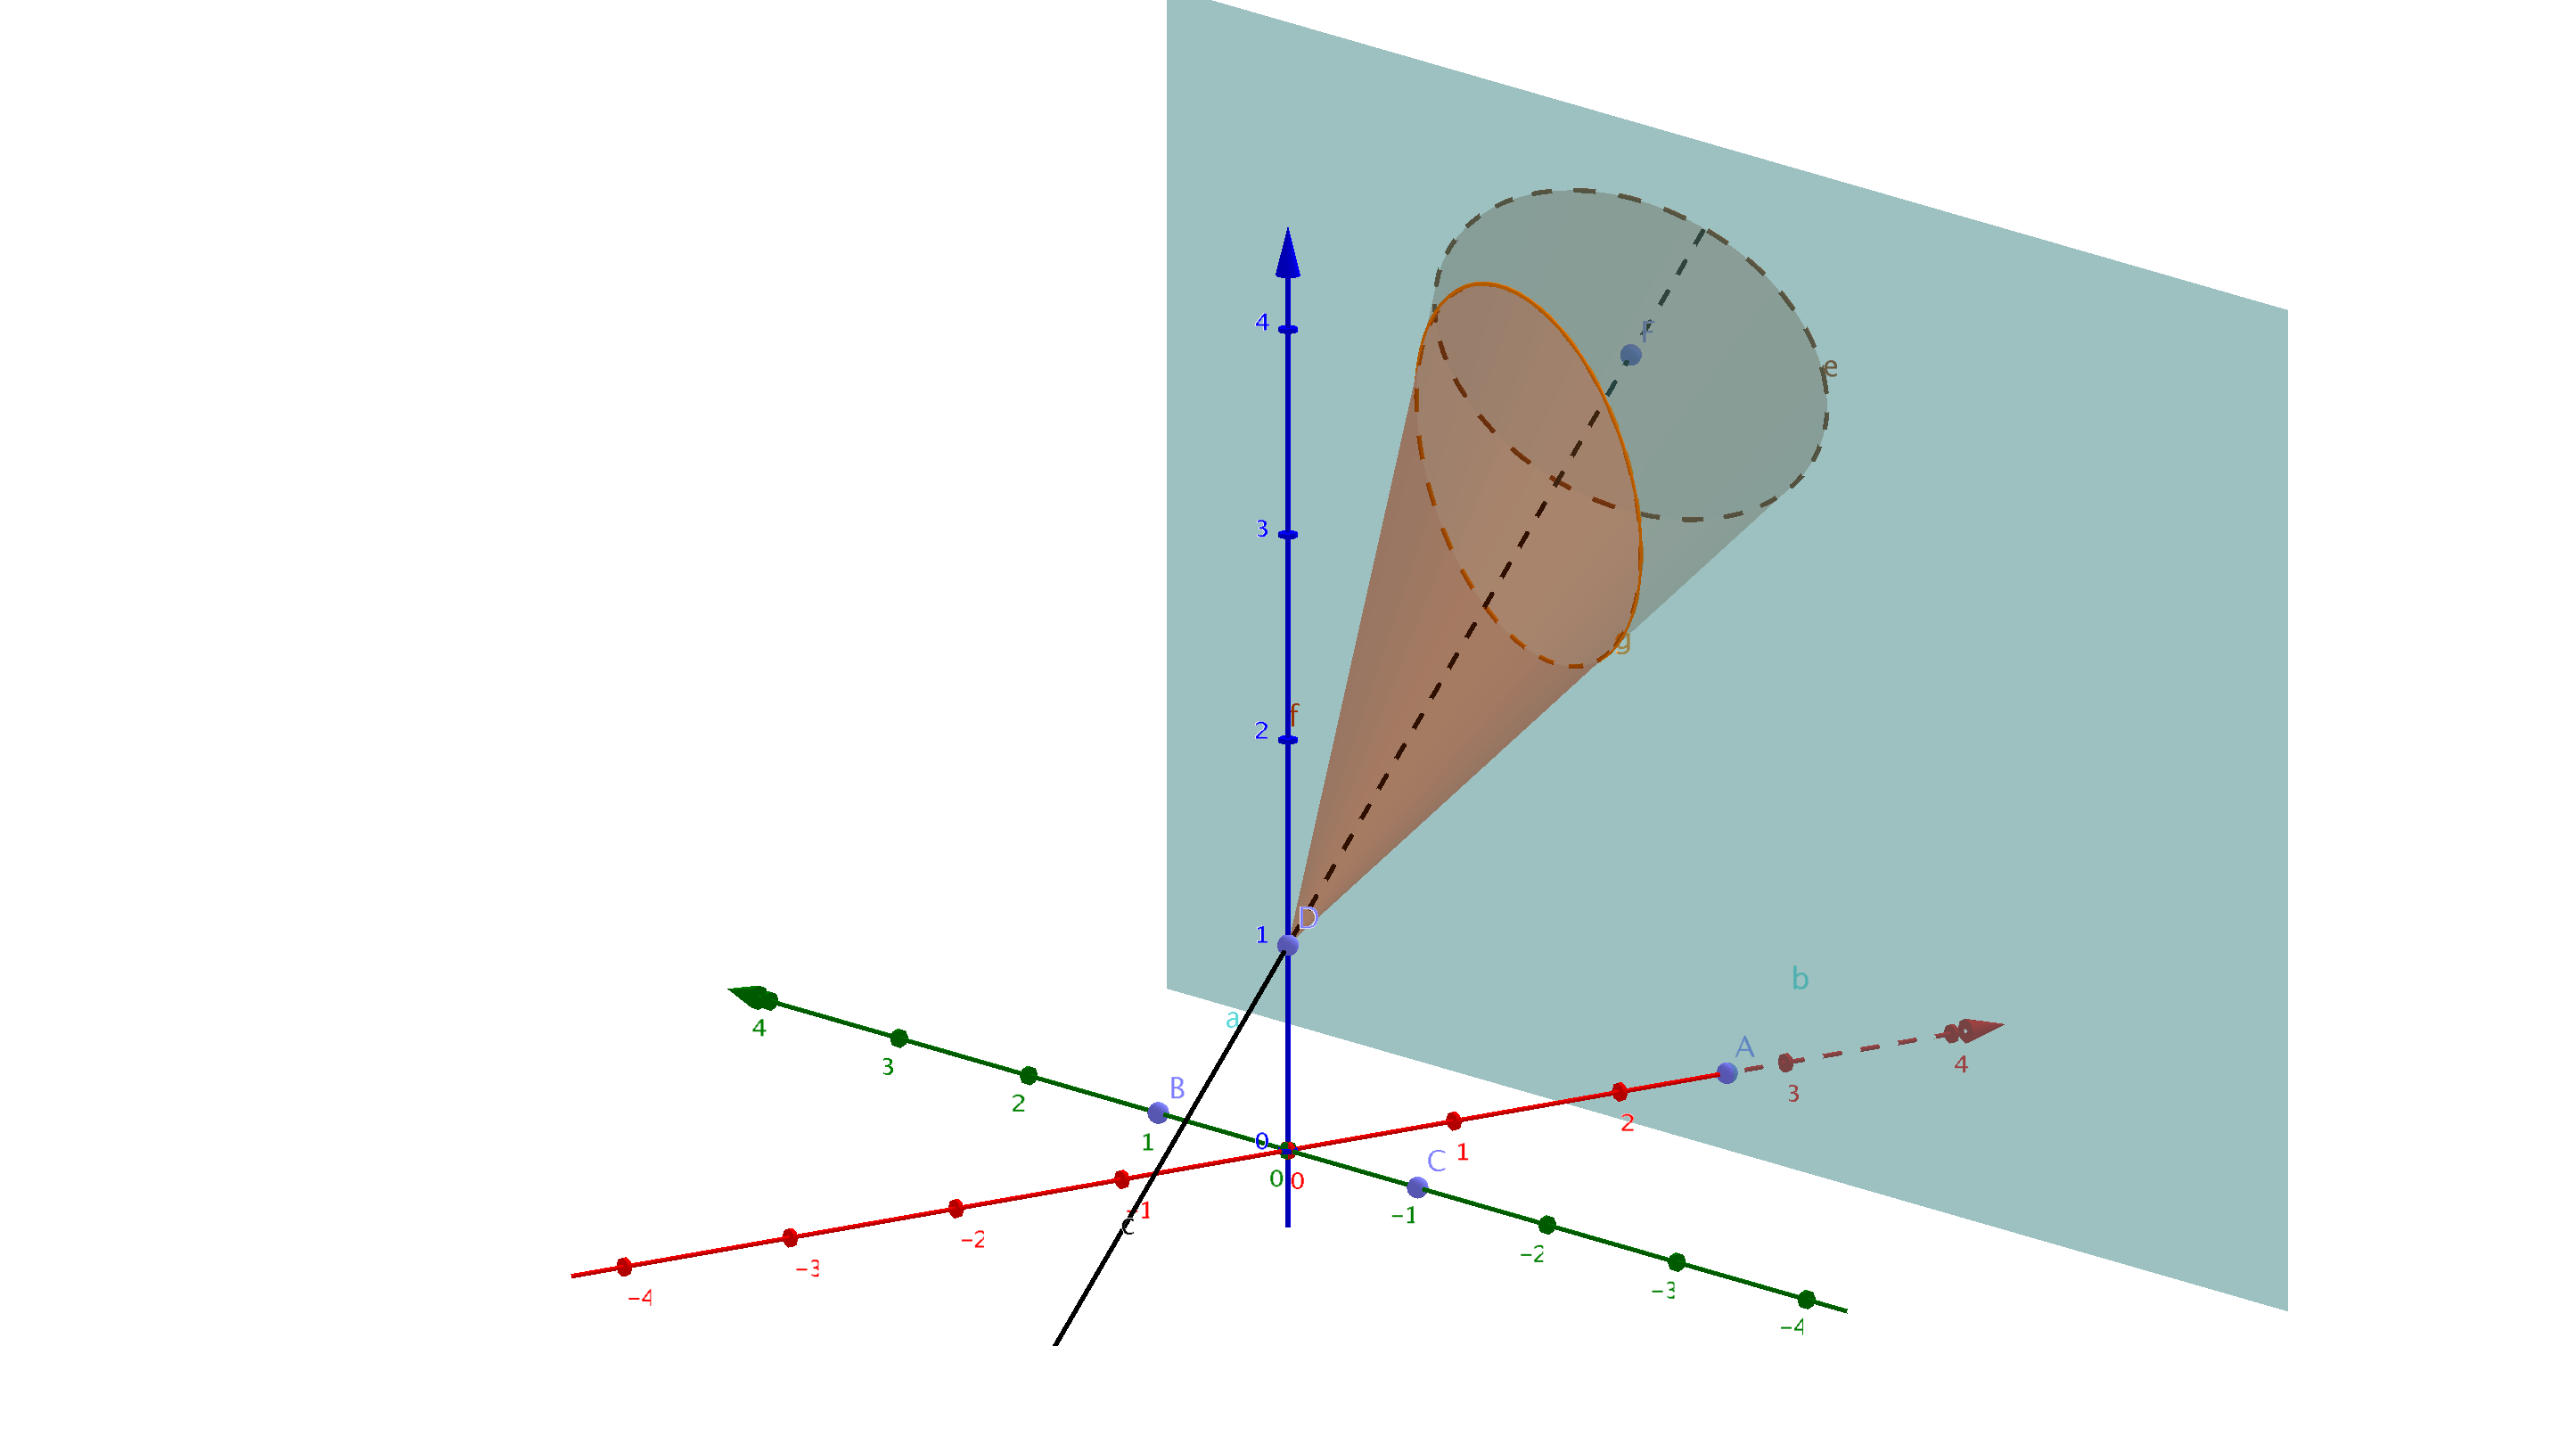
\includegraphics[width=1.0\linewidth]{figures/prop600GoodOffSensor.png}
\caption{The same as figure \ref{fig:ScatFrame1} from a different angle.}
\label{fig:ScatFrame2}
\end{figure}

The propagation of scattering errors to different frames is all well and good. However you must be able to determine the amount of scattering expected at each point.

First the total radiation length must be determined for the track's trajectory. TGeo volumes are used to describe the full detector system including the radiation length. The track is assumed to propagate through each volume at the appropriate incidence to determine the correct radiation length at each point. Two things must be determined to model scattering.

First the variance at each point must be determined. To determine this the total variance of the trajectory must be calculated. The total variance is calculated using the radiation length and beam energy. This is were the Highland formula comes in. The Highland formula relates the radiation length percentage and beam energy to a scattering RMS. One important characteristic of the Highland formula is its non linear properties: The radiation length calculated must be for the full system and then split between each point used to model the scattering. 

Second the position of the scatterers must be determined. This depends on the radiation length and size of the volume to model. If the volume is thin then it can be assumed a thin scatterer. A thin scatter will have no displacement through the material but some angular displacement. So all the radiation length is located at that point. The red measurement dots on figure \ref{fig:LinkJac} are modeled this way. The variance at this point is the total variance weighted by the fraction of radiation length at this point relative to the total radiation length.
A thick scatterer will have some displacement due to scattering within the material and can be viewed as the combination of many thin scatterers. If you propagate the error associated with each thin scatterer which makes up the thick scatter then it can be shown that a thick scatterer can be modelled by two thin scatterers. The location and allowed variance of the kinks is determined using the relations

\begin{multicols}{2}
\begin{equation}
 s_1 = s_0
\end{equation}
\begin{equation}
s_2 = \overline{s} + \frac{\Delta s^{2}}{\overline s - s_1} 
\end{equation}
\begin{equation}
\theta_{1}^{2} = \theta^{2}\frac{\Delta s^{2}}{(\Delta s^2 + (\overline s - s_1)^{2}} 
\end{equation}
\begin{equation}
\theta_{2} = \theta^{2}\frac{(\overline s - s_1)^{2}}{\Delta s^2 + (\overline s - s_1)^2} 
\end{equation}
\end{multicols}

were $\theta^{2}$ is the total variance, $s_0$ as the initial position of the scattering volume and 

\begin{multicols}{3}
\begin{equation}
\theta^{2} = \int_{a}^{b} \theta_{i}^{2}
\end{equation}
\begin{equation}
\overline{s}=\frac{\int_{a}^{b} s_i \theta_{i}^{2}}{\theta^2}
\end{equation}
\begin{equation}
\Delta s^{2} = \frac{\int_{a}^{b} ( s_i  - \overline{s})^2 \theta^{2}_{i}}{\theta^2}
\end{equation}
\end{multicols}

were T=b-a which is the start and end position of the scatterer volume. 
Integration can be used to work out the parameter values for any inhomogeneous volumes. Most situation will have blocks of homogeneous material one after the other. In this case the above equation can be treated as: 

\begin{equation}
 \overline{s} = 0.5 \sum_i \frac{T_i}{X0_i} 
\end{equation}

\begin{equation}
 \Delta s^{2} = \sum_i \frac{\frac{1}{3} T^3 - T^{2}\overline{s} + T\overline{s}^{2}}{X0_i} 
\end{equation}

\begin{equation}
 norm =   \frac{T_i}{X0_i} 
\end{equation}

were T is the thickness and the summation is over all homogeneous volumes.  This allows the correct modeling of the radiation length for the full particles trajectory. 

If a more detailed radiation length calculation is needed then the tracks actual trajectory through the full TGeo volumes space can be used. However in all examples this is not required. Care must be taken that the TGeo volumes described contain the sensor hits. Since a transformation between local and global can move the hits outside these volumes. The current simple radiation length calculations do not suffer from the this problem since they always travel through each blocks' centre.

Dead material which should be added as radiation length but is of no interest is identified in the gear file with $ID>99$. One example in section \ref{example} demonstrates this.



\subsection{Add global parameters}
\label{gloPar}
The addition of global parameters is used to determine alignment corrections. However this can be used for any variables which are common to all tracks. Note this in contrast to local parameters which vary from track to track.  Alignment is simply the determination of the correct transformation from local to global frames for each sensor. 

\begin{figure}[H]
\centering
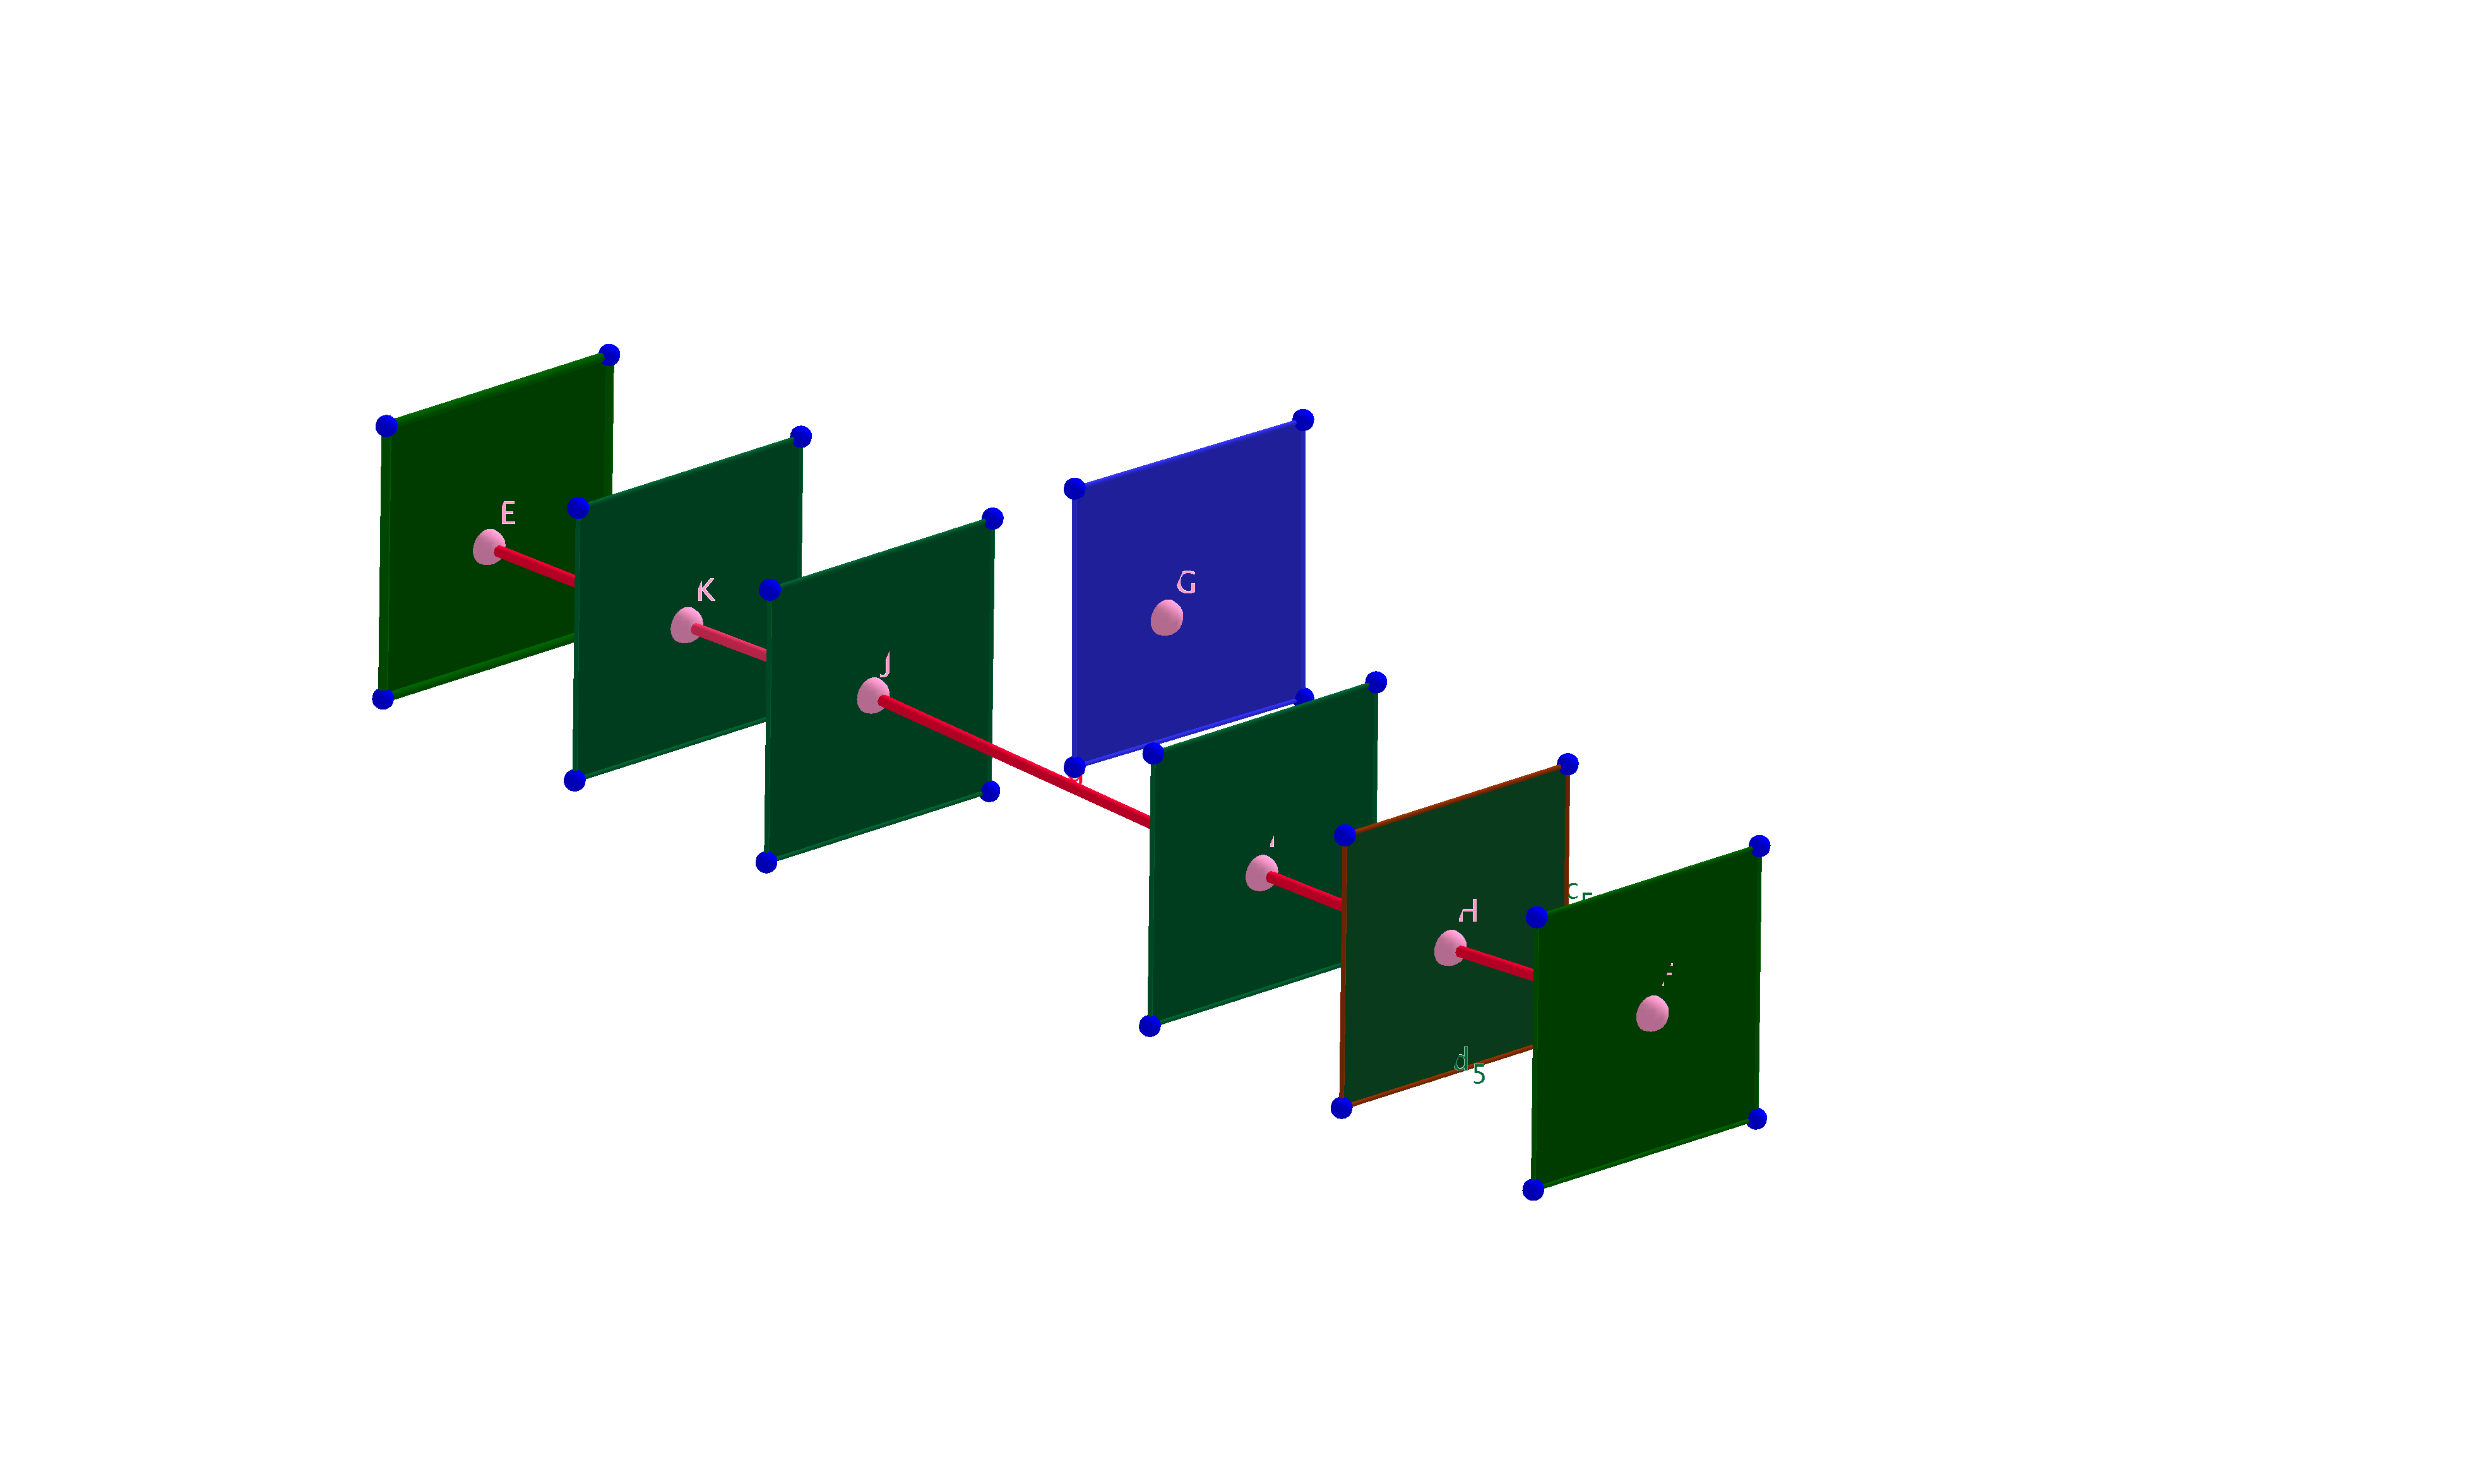
\includegraphics[width=1.0\linewidth]{figures/MisAlignStraight.png}
\caption{Illustration of misalignment with DUT. The transformation of the local DUT frame to the global frame must be wrong so the corrections must be found.}
\label{fig:MisAlign}
\end{figure}

Figure \ref{fig:MisAlign} illustrates a clear problem with the description of the sensor in space. The corrections needed are assumed to be the transformation between global and local frames which minimizes the residual weighted with errors for all tracks and planes.

A link between the local frame residual and alignment parameters which define the transformations must be determined. The alignment parameters are defined $(X,Y,Z, \alpha,\beta,\gamma)$ which are the offsets in the global frame and the rotations defined in each frame of the rotations applied before it. This last point is important: The corrections to the rotations must be determined in the frame reached before that rotation is applied. So the $R_X$ (Rotation round X axis) matrix correction must be determined after you have rotated round the Z axis. This can be dealt with in two ways: 

1) Determine the corrections for each rotation in the frame it is applied then rotate to the local frame. 

2) Only apply large rotations and parity transforms before you apply corrections. 

The second approach is taken with all X/Y rotations applied in the initial rotation matrix. Note rotation round the Z axis is also permissible since this is the first matrix to be corrected. The parameters' change is related to change in position of a point in the coordinate system by the  \emph{point correction matrix} $\hat{PC}(X,Y,Z, \alpha,\beta,\gamma)$:
\[ \left( \begin{array}{cccccc}
1 & 0 & 0 & 0 & relZ & -relY \\
0 & 1 & 0 & -relZ & 0 & relX  \\
0 & 0 & 1 & relY & -relX & 0   
  \label{eq:PC}
\end{array}
 \right)\] 

This matrix will create a correction vector at the location and coordinate system specified by the relative positions. 
The relative positions are defined as the global predicted position without offsets. This is done so the order of magnitude of the rotation is correct. So defined as:

\begin{equation}
 \overrightarrow{rel} =   \hat{R}\overrightarrow{L} 
\end{equation}

The predicted positions used are the pattern recognition tracks and not the GBL fit.  

\begin{figure}[H]
\centering
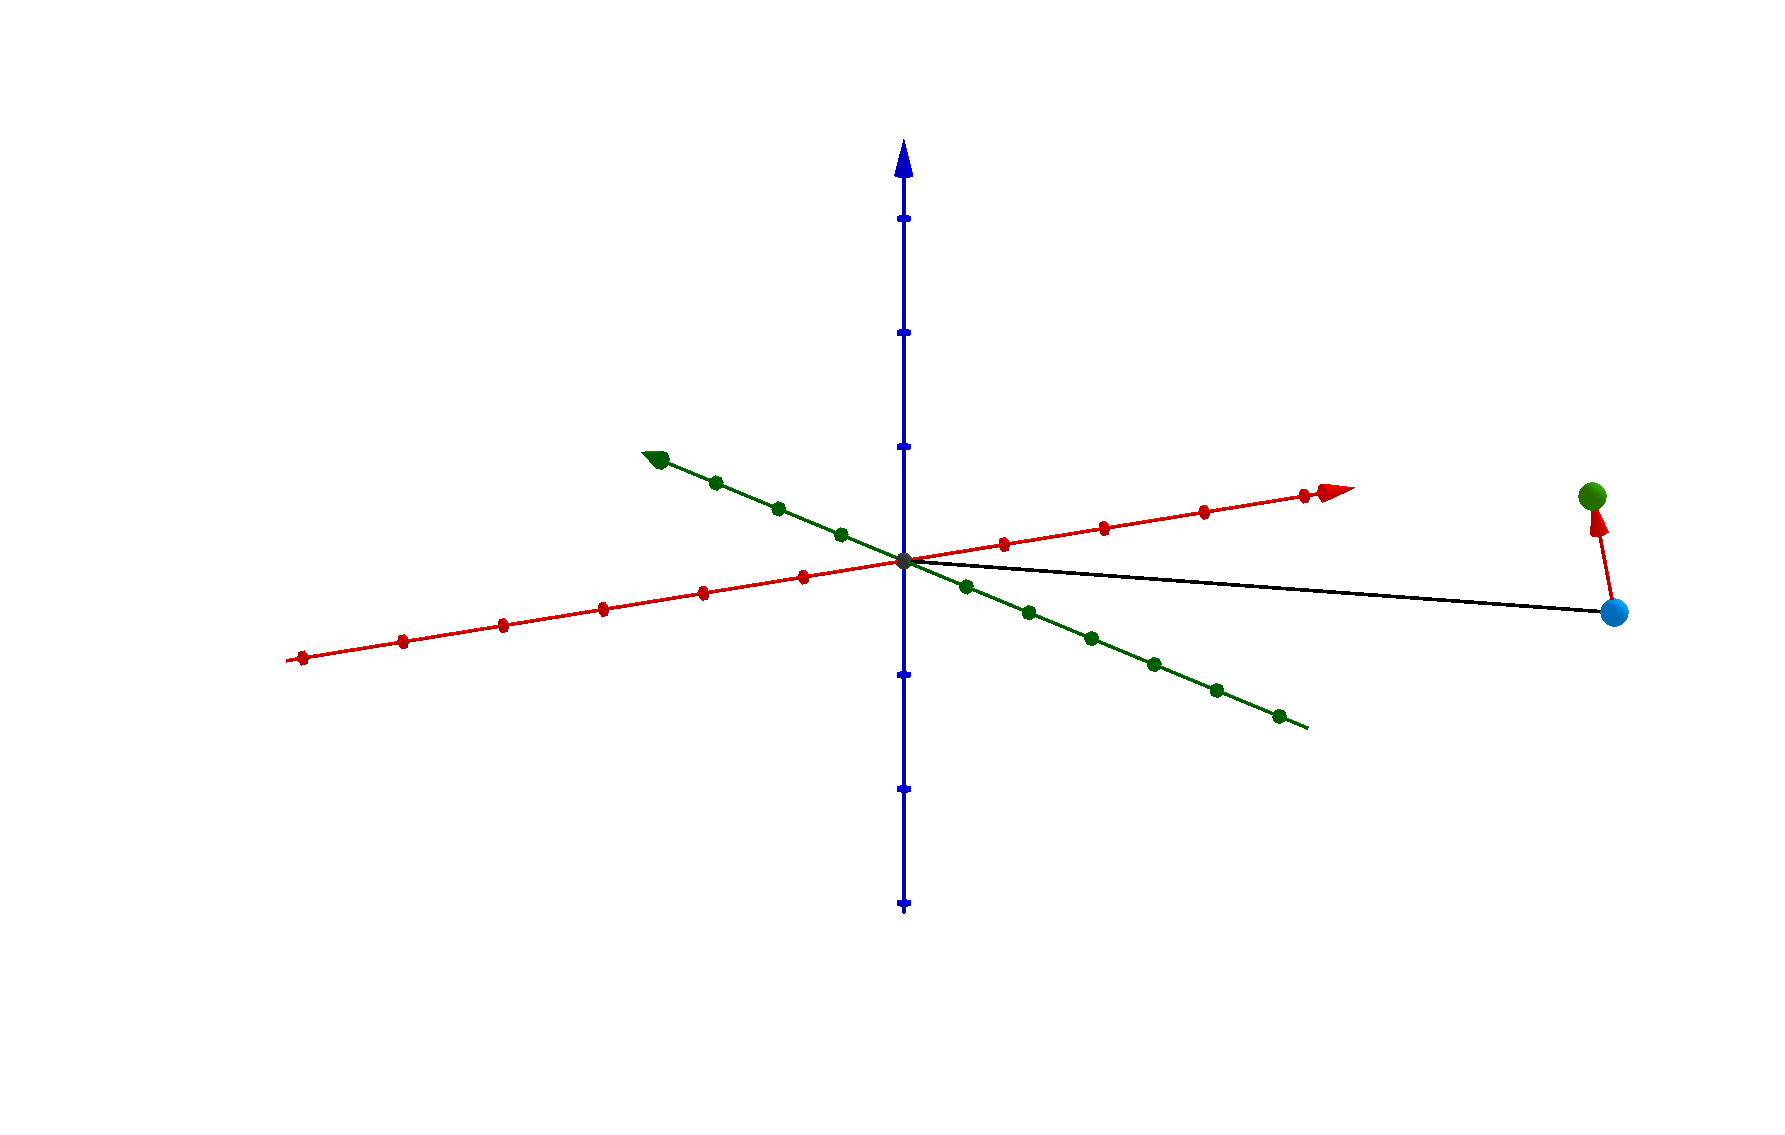
\includegraphics[width=1.0\linewidth]{figures/corrAlign.png}
\caption{The point correction matrix for a particular relative position. The vector is the correction to apply to this point given a certain $(X,Y,Z, \alpha,\beta,\gamma)$ change in the coordinate system.}
\label{fig:CorrMatrix}
\end{figure}

The correction vector will not give the change measured on the plane from moving the track. To estimate this the correction vector must be considered moving a track rather than a point. This is done using the \emph{track correction matrix} $\hat{TC}(\overrightarrow d, \overrightarrow n )$ 
\begin{equation}
  I -  \frac{\overrightarrow d \times \overrightarrow n}{\overrightarrow d . \overrightarrow n}\\
  \label{eq:TC}
\end{equation}

which will move a track by a particular displacement and determine how this changes the intersection with a plane. 

\begin{figure}[H]
\centering
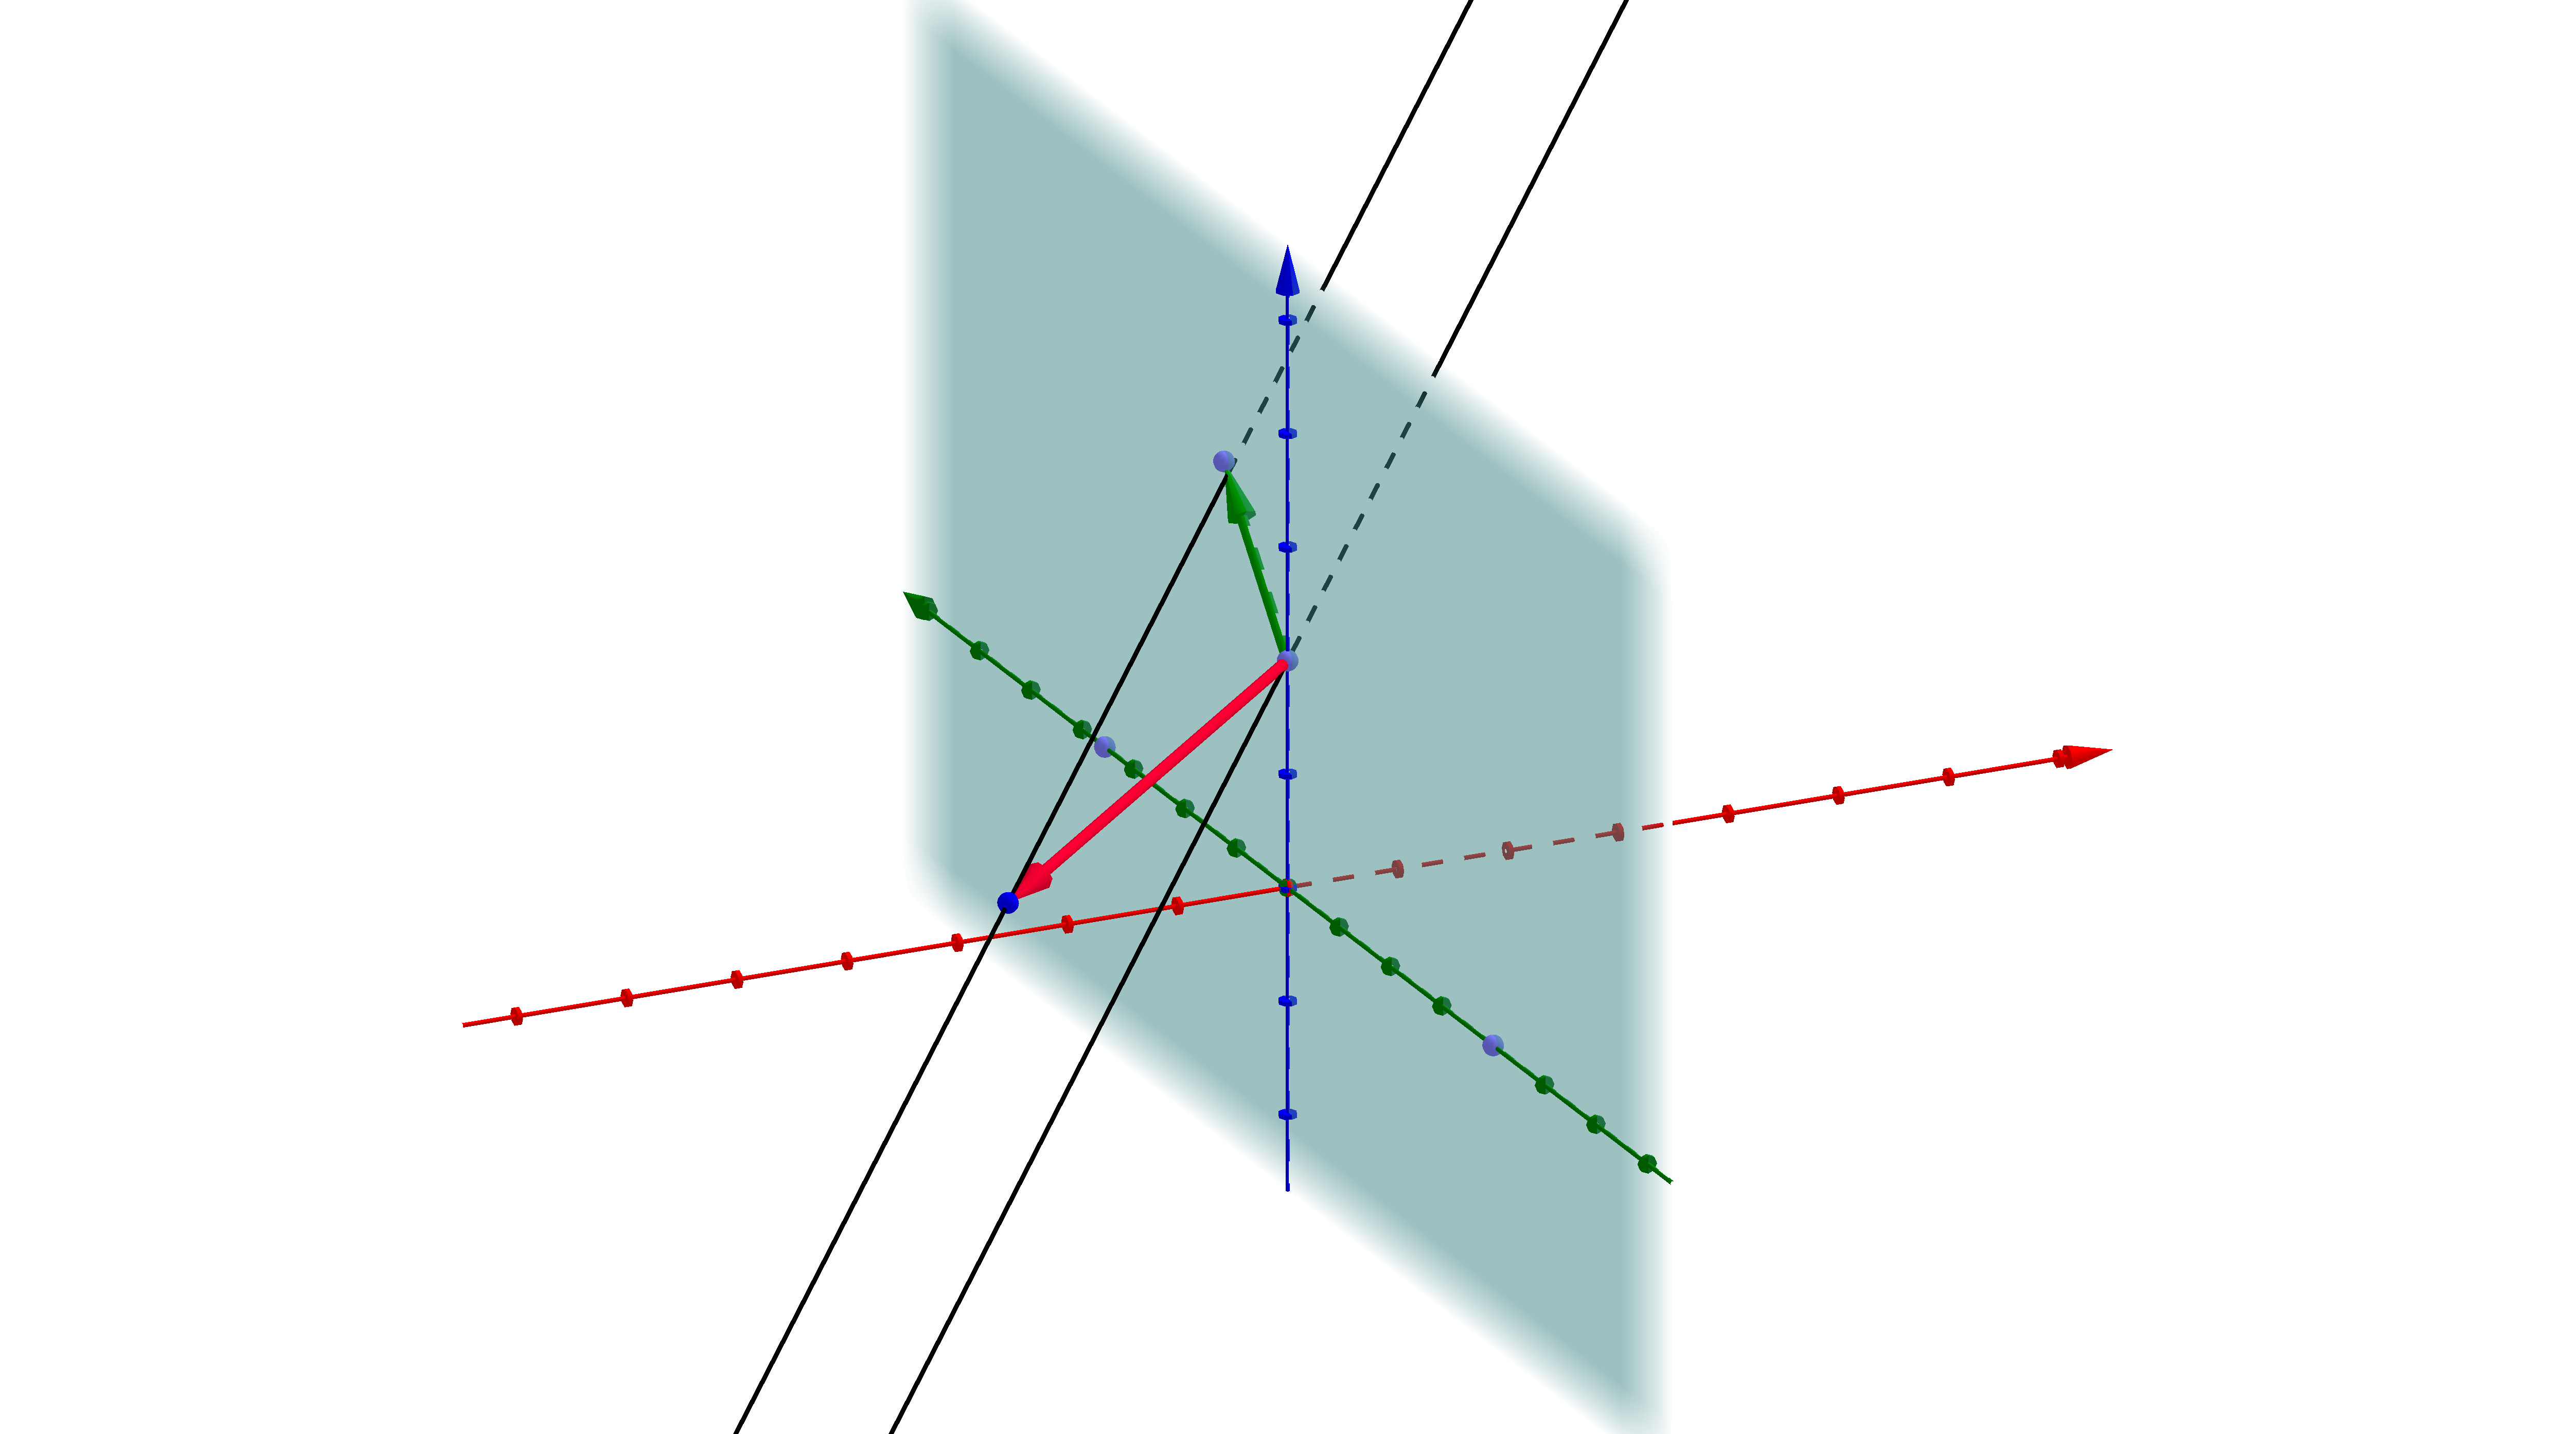
\includegraphics[width=1.0\linewidth]{figures/alignBigger.png}
\caption{The track correction matrix will take as input the track displacement given in red. It will then determine the green vector which is the change on the plane due to that displacement}
\label{fig:TC1}
\end{figure}

\begin{figure}[H]
\centering
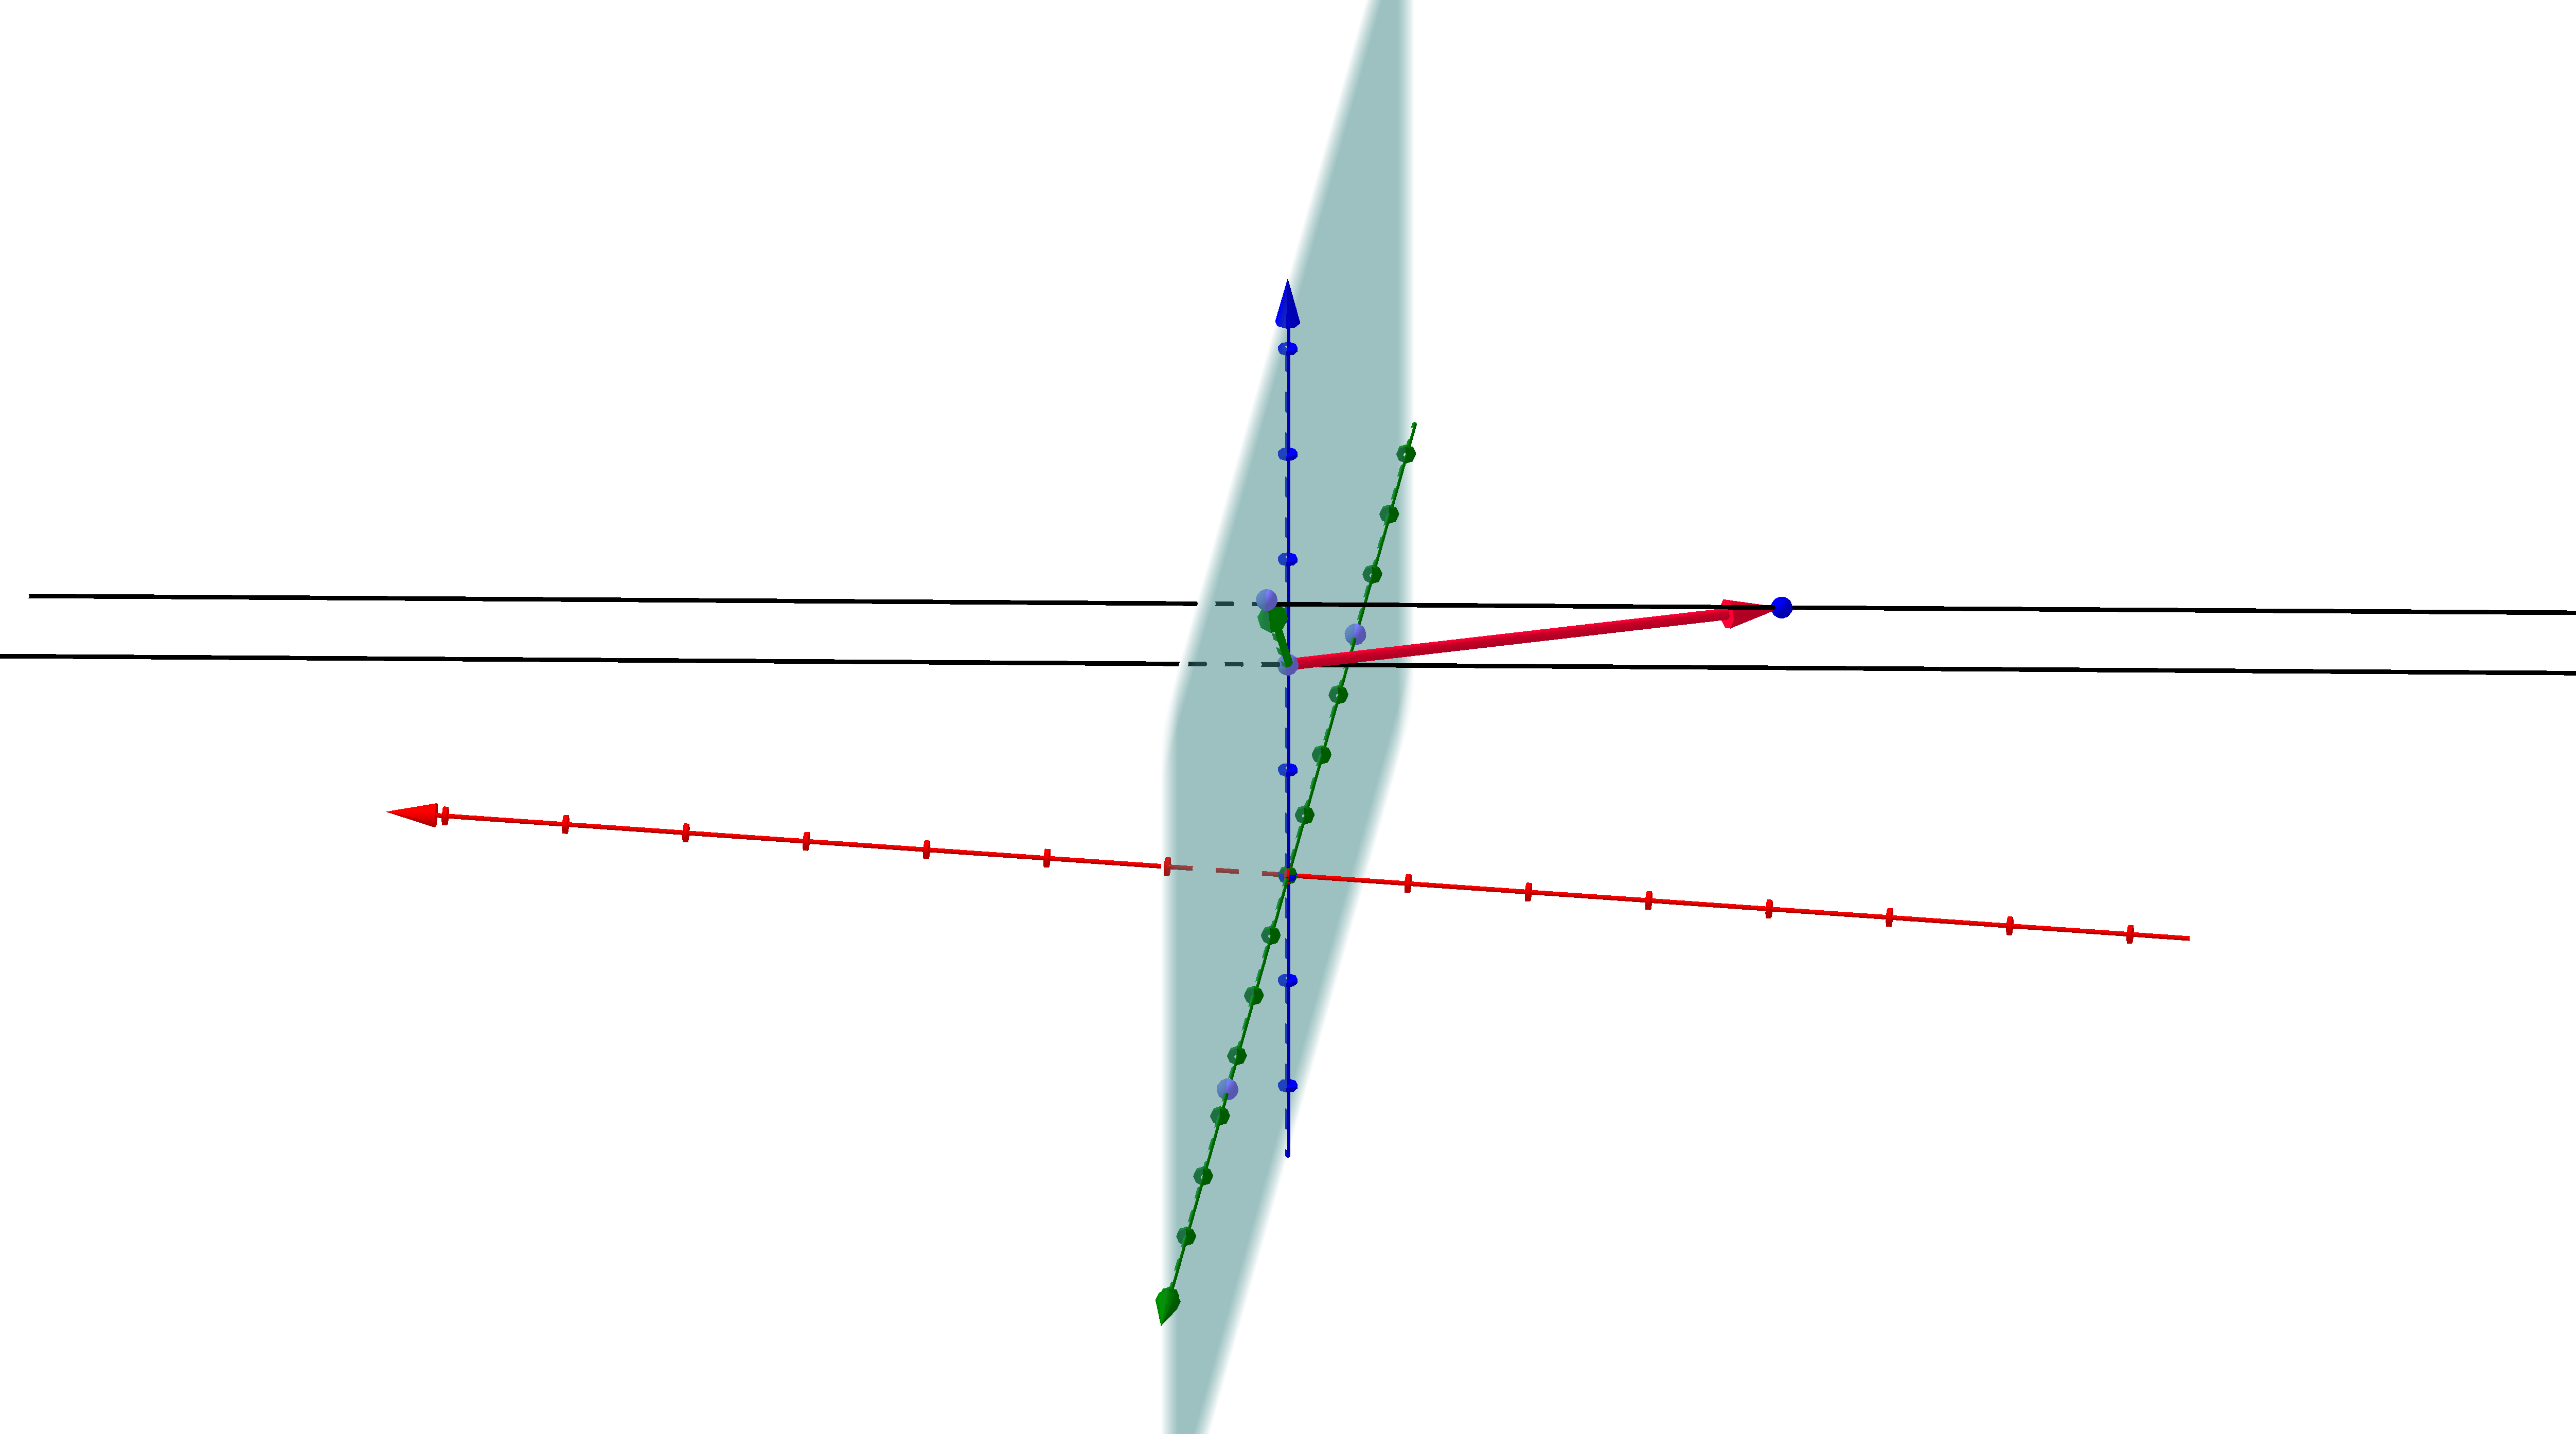
\includegraphics[width=1.0\linewidth]{figures/alignmentBigger.png}
\caption{Same as \ref{fig:TC1} but from a different angle. The green vector is on the plane surface.}
\label{fig:TC2}
\end{figure}

The final full body alignment can determined by combining TC and PC. This will relate the change in global alignment parameters to change on a plane. The plane described is in the global frame. Therefore the vector on the plane must be rotated into the local frame of the sensor. This frame will of course have zero Z displacement since it should be on the sensor surface. The final matrix passed to millepede:

\begin{equation}
\hat{R^{T}} \hat{TC} \hat{PC} 
\end{equation}

were the transpose of the rotation matrix is the inverse.

\subsection{Add local parameters}

Local parameters are added in the same way as global. However the variables of interest will vary from track to track. Local parameters have been added to the software to determine kink angles at a particular point.

Kink angles can be estimated using the plane ID=271 in the gear file at any detector position. This method could be used to determine the radiation length of the detector system in the future. However it is only in the initial stages of development and should be used with caution.






\clearpage

\chapter{Further Work }
\label{chp:furtherwork}
\input{parts/furtherwork.tex}
\clearpage

\chapter{Guide to Resonance Search}
\label{chp:guide}
\section{Introduction}
This is designed to be an introduction to any analysis and will cover some of the basic ideas needed. However a focus on the the VH analysis give \href{https://cds.cern.ch/record/2054042/files/ATL-COM-PHYS-2015-1180.pdf}{here}

\section{Theory and past searches}
Need to be filled in after going through theory course again.

\section{Data and MC samples}

Pileup must be taken into account. This is done via reweighting. The quality of the data is validated using the GRL and DQ flags. The simulation of signal and background can be viewed in \ref{section:Simulation}. 

The k-factor is a factor which relates the leading order to the error compared to the full calculation. The filter term is to relate the number of events expected to the number produced. 

To begin to discuss physics objects you need to begin at the xAOD root files created by simulation and data. You can see all the collections and type in an xAOD using:

checkxAOD.py 


The ATLAS Muon Combined Performance Group define muons using a series of cut points, this is done for inner detector and muon spectrometer. Both the ID and MS are used in combination to determine the pt and mass of the muon. Note the pt and resolution depend on many factors (magnetic field, scattering, intrinsic resolution), therefore momentum scale and resolution corrections are also applied. This makes the MC and data follow the same distribution. These were determined using the J/$\psi$ (c$\bar{c}$)/Z resonance.  Reconstruction efficiency is allowed to vary with a scale factor which is the ratio of MC/data. This if course depends of pt and $\eta$. 

Isolation criteria for leptons is needed since semi leptonic/hadronic decays are the main source of non-prompt/misidentified leptons. A tight cut is performed on each lepton by constructing the energy for the track/Calo object inside a R=0.2 cone and then doing a cut which depends on $p_t$ and $\eta$. The energy must be over this cut value. A variable R cut is also performed on tracks only for the loosetrackonly requirement. This reduces the size of the cone since the Z $\rightarrow$  ll cone will reduce in size for higher pt.   


Calorimeter jets are corrected by adding muon inside jet to jet. $H \rightarrow b \bar{b}$ reconstructed with 1.0 large R jet, which focuses on pt > 250 GeV since less than this will be in a larger jet. Smaller R jets are used for Etmiss which must use a set eta and pt > 20 GeV for JES calibration to be valid. Note the JES must be compared to MC since the real detector will have some energy loses. This is also an additional uncertainty for the final fit.  To reduce jets not from the primary vertices other than hard scattering vertex JVT recommendations for pt < 50 GeV smaller R jets is used.  JVT is used to reduce pile up by determining the primary vertex and then determining the amount of energy which comes from this. 

Overlapping jets with electrons are removed if within R < 0.2 

\section{Triggers}
The trigger efficiency depends on a particular sample. A sample here is a selection of cuts after requiring these triggers.  The efficiency is determined by taking a selection of events from the sample and running this through the trigger. The efficiency is just the ratio before and after the trigger. Note the efficiency will depend of some observable, e.g VH mass. A scale factor must also be used to determine the different between MC and data. 

\section{Selection}

The number of VHLoose lepton number is varied to keep the 0/1/2 lepton channel orthogonal. 

In the two lepton channel the muon momentum resolution deteriorates at high pt so the pt is scaled by $\frac{m_{ZZ}}{m_{\mu \mu}}$.

W mass constraint used in the 1 lepton channel to determine neutrino pt. 

Geometric cuts are used in the 0 lepton channel. 

After these kinematic cuts then the H $\rightarrow b\bar{b}$ is exploited to increase sensitivity. This is also used to define control regions. This is done looking at the mass and number of b tags.  

\section{Multijet}


\section{Nuisance Check update (NP Pruning)}


\section{CMake Introduction)}
%INCLUDE >>> Will run cmake code from another file
%LIST >>> Will do a variety of task with lists. APPEND will create a list.
%To see a list of FIND_PACKAGE entries do: cmake --help-module-list  
%FIND_PACKAGE had two modes: 1) module => searches CMAKE_MODULE_PATH  2)Config
%
%Will set the following variable:
%  <name>_FOUND  // true iff the package was found
%  <name>_INCLUDE_DIR   // a list of directories containing the package's include files
%  <name>_LIBRARIES     // a list of directories containing the package's libraries
%  <name>_LINK_DIRECTORIES  // the list of the package's libraries
%  
%  .a static or .lib (windows) => so code compiled within
%  
%  .so dynamic .dll (windows) references to the code given outside
%  
%  Need to link lib with EUTelescope with 
%  -DBoost_NO_BOOST_CMAKE=ON

\section{CxAODMaker} 



\section{Abbreviations}
\begin{itemize} 
\item EDM $\rightarrow$ Event Data Model 
\item GRL $\rightarrow$ Good Run List 
\item JES $\rightarrow$ Jet Energy Scale
\item JVT $rightarrow$  Jet Vertex Tagger
\end{itemize}





\clearpage

\bibliographystyle{plain}
\bibliography{../bibliography}
\clearpage

\end{document}

